


% Trenger "Table of abbrevations"
% 	- LTP, LTD, STDP
% 	- "spike" ? (at det betyr Action potential)?
% 	- SANN  - spiking ANN
% 	- SN 	- Spiking Node, a node in SANN.
% 	- KANN, KN.
% 	- LIF neuron: 	Leaky--Integrate and Fire  neuron




% Eller kanskje eg treng stikkordsregister: Trenger:
% 	- Det over og:
% 	- axo-axonic synapses
%
%






\documentclass[a4paper,11 pt]{report}





% TODO TODO TODO TODO TODO TODO TODO TODO TODO TODO TODO TODO TODO Skriv inn navn på alle refererte enkeltkapittel, i bibliografi.bib TODO
% TODO TODO TODO TODO TODO TODO TODO TODO TODO TODO TODO TODO TODO Endre rapport i NEVR3003, og legg det inn som appendix. Referert til i "The BiologiskeSystemet" -- kapittelet.
% 																	TODO Gjør om denne, slik at en kybber kan lese den. Definer uttrykk som LTP, LTD, (AMPA?), ATP,  ...

%%%%%%%% KRISTOFFER sine usepackage (i diplomen)
%\documentclass[a4paper, english, 12pt]{article}
%\usepackage[utf8]{inputenc}
%\usepackage[T1]{fontenc} %%
%%%\usepackage{babel}
%\usepackage{graphicx}
%\usepackage{subfigure}
%\usepackage[amssymb,binary]{SIunits}
%\usepackage{amsmath,amsfonts,amssymb,textcomp,varioref}
%\usepackage{listings} % Er lenger nede..
%\usepackage{times}
%\usepackage{nomencl}

%%%%%%%%% Mine fra før dette:

\usepackage[utf8]{inputenc}
\usepackage{graphicx} 

% sudo apt-get install texlive
\usepackage[font=small,format=plain,labelfont=bf,up,textfont=it,up]{caption}

\usepackage{amsmath}
\usepackage{mathrsfs} %brukt for krølle-L : laplace

\usepackage{subfig}   % for subfigures.
\usepackage{listings} %for c++ kode
\lstset{language=c++}

%\usepackage{pstricks} % For teikning. 		FOR mykje styr å lære..
%\usepackage{pstricks-add}
 %\let\psgrid\relax %XXX Fjærner GRID på alle pstricks teikninger. (global removal)

%\usepackage{epstopdf} % for å få med eps i pdf-latex (?)



%Kanskje dette er naudsynt? For metapost:
%\DeclareGraphicsRule{*}{mps}{*}{}


%%%%%%%% Fra Kristoffer sin master:
%\lstset{ %
%basicstyle=\footnotesize,       % the size of the fonts that are used for the code
%numbers=left,                   % where to put the line-numbers
%numberstyle=\footnotesize,      % the size of the fonts that are used for the line-numbers
%stepnumber=1,                   % the step between two line-numbers. If it's 1 each line will be numbered
%numbersep=5pt,                  % how far the line-numbers are from the code
%showspaces=false,               % show spaces adding particular underscores
%showstringspaces=false,         % underline spaces within strings
%showtabs=false,                 % show tabs within strings adding particular underscores
%frame=single,                % adds a frame around the code
%tabsize=3,                % sets default tabsize to 2 spaces
%captionpos=b,                   % sets the caption-position to bottom
%breaklines=true,                % sets automatic line breaking
%breakatwhitespace=false,        % sets if automatic breaks should only happen at whitespace
%escapeinside={\%*}{*)}          % if you want to add a comment within your code
%}


\author{Per R. Leikanger}
\title{Development and Assessment of a Novel Model for Artificial Neural Networks}
\date{\today}     



\begin{document}   

\maketitle

%TODO 
% 	For kvart plott: Skriv at det er fra log-filene fra implementasjonen.


%Når det gjelder skriving, så er det veldig effektivt med uttrykk som "the rationale behind the choise of letters $n$,$s$, and $a$ is explained in chapter 3." 	Bruk dette! 
%Frampeik, med litt mystikk som impliserer at eg veit meir enn leser. (Hugs norsk fra grunnskulen: frampeik er bra!)
%I tillegg til at det impliserer at eg har tenkt mykje over saken, så syr det teksten bedre sammen!

\emph{Om oppgaveteksten:}
Les meir grundig det som står på toppen. Den punktinndelte oppgava på bunnen gir følgende notater:

Eit poeng: "(NB: Hold deg innenfor oppgaven,du kan ikke regne med å få
kreditt for arbeid som går på siden av oppgavens uttalte fokus)."
------> Skriv kvifor eg har implementert simuleringa så nøyaktig. Begrunn dette, for å få uttelling for det i karrakteren. 

Hold også eit auge med skrivet eg fekk fra Øyvind S.: Korleis gjennomføre prosjekt. Spesiellt i forhold til innledning er dette viktig!
	\emph{Pkt. 1}
Oppgaveteksten seier: "Gi en oversikt over eksisterende modeller for ANN som representerer både fyringsrate og -tidspunkt. 
Legg spesielt vekt på forhold som kan knyttes til stabilitet under læring og/eller tilbakekobling ("recurrent ANN")."

Første setninga kan tolkes, men eg trur tolkininga som går på at det er en modell som representerer begge er mest rett (BÅDE). 
Trur ikkje det er nokon modell som gjør dette. Kan skrive dette, så skrive om modeller som representerer fyringsrate ELLER -tidspunkt. (fANN, SANN).


	\emph{Pkt. 2}
"Beskriv det nye konseptet, og påpek hvordan dette skiller seg kvalitativt fra tidligere kjendte metoder."

Tolkning: tidligere kjendte metoder - tidligare modeller som representerer tidspunkt for fyring. Bare SANN!

Ellers er dette punktet rett--fram.

	\emph{Pkt. 3}
"Foreta en sammenlikning av det nye konseptet og konkurrerende metoder. Evalueringen kan baseres på et antall konkrete scenarier(mhp. inngangsdata osv.)."

Tolkning:
Konkurerende metoder er andre metoder som også representerer tidspunkt for spikes. Dette er bare SANN (kanskje ta med ulike implementasjonsmetoder av SANN? Timedriven/eventdriven?)
Eg tenker at eg ikkje får tid til å gjøre en omfattende sammenligning av effektivitet, så sammenligner med bakgrunn i implementasjon. 

Sammenligne litt for effektivitet (for ulike oppsett).

Sammenligne tematisk? Skrive at eine er Moore, andre Mealy auromata?


\tableofcontents



%Oppgava sei:
%2) Describe the new concept, and point out how this differs quantitatively from earlier known models.
% MERK:   .., OG beskriv how this differs from earlier known models. TODO Gjør dette eksplisitt.
% Peik på kor, i innledning.



%Intro: utvida innholdsfortegnelse
\chapter{Introduction}  			%XXX KAPITTEL

% KAPTITTEL : Introduction
%TODO Må skrives: sett av 0.7 dag til dette.

%Todo Skriv kvifor eg 'cite' kapittel til de ulike bøkene. Bøkene er ofte så store at uten dette blir referansene memingsløs..




%
% 	- Utvida innholdsfortegnelse.
% 	- Skrive at eg har, og vise til kor eg har    ->  svart på de ulike aspektene ved oppgaveteksten.
% 	- Skrive eksplisitt om oppgaveteksten.
% 	- 
% 	- 

\newpage
\section{Oppgavetekst}
In most artificial neural networks (ANN),  a neuron's output variable can be said to represent the time varying firing rate (i.e. number of action potentials per time unit) of its biological equivalent.\\
In this domain, there is no representation of firing time and other aspects related to causality and stability that appear to be central to the learning process in a biological neural network.
 
 In this project, you will develop a new concept for ANN that takes into consideration both firing rate and firing time, and compare it with the existing model known as Spiking ANN (SANN).
 \begin{itemize} 
  \item[1] Give an overview of existing ANN models that represents both firing rate and firing time. Emphasis should be put on factors that can be related to stability for synaptic plasticity (learning) and/or feedback ("recurrent ANN").
  \item[2] Describe the new ANN concept, and point out how this differs qualitatively from previous models.
  \item[3] Compare the new concept with competing methods. The evaluation may be based on a number of specific scenarios (with respect to input data etc.).
 \end{itemize}

 Supervisor:      Øyvind Stavdahl, Associate Professor, Department of Engineering Cybernetics, NTNU\\
                  Professor Gaute Einevoll, Department of Mathematical Sciences and Technology, Norwegian University of Life Sciences.
\newpage

\section{Abstract}
Husk: tittel er ekte delmengd av abstract, som er ekte delmengd av introduction, som er ekte delmengd av rapport.

\section{Introduction}

In this text many 

% XXX Følgende er kjempeviktig å ha med:
In this report the convention used by Rolls and Treves in ``Neural Networks and Brain Functions'' will be used. 
For any transmission through a synapse between neuron $j$ and neuron $i$, we define the synaptic strength $w_{ij}$.  % TODO Skriv heller: "..through a synapse FROM neuron $j$ TO neuron $i$, we .."
Note that the first subscript refers to the recieving neuron and the last subscript to the presynaptic neuron (the signalling neuron) \cite{TrevesNeuralNetworks}.
This convention will be used in this text. 
% XXX XXX XXX  (bra skrevet er det og)






%TODO NEVN action potential i innledning! XXX VIKTIG!




%(tidligere) KLADD:
%Recently, there have been a strong focus on the timing of spikes. There are two reasons behind this.
%The first is connected to synaptic plasticity. 
%In 1987, Gustavsen et. al. found that synaptic plasticity could vary as a function of the postsyn
%Synaptic plasticity can be divided in two groups, Long Term Potentiation (LTP) causing an a lasting increase in the synaptic weight and Long Term Depression (LTD) causing a lasting decrease in the synaptic weight.
%Gustavsen et. al found in 1987 that the synaptic plasticity vas a function of the postsynaptic depolarization at the time of transmission. 
%The synaptic plasticity varied from a strong LTP to a strong LTD as a result from a single transmission\cite{Gustafsson03011987}.
%%Dette ble også overført til ANN

%We can say that, statistically there is a correlation between the presynaptic depolarization after a synaptic transmission, and the relative timing of the postsynaptic action potential. %ELLER NOKE: RYDD OPP XXX XXX
%If we view this statistically, we can say that the timing of the presynaptic action potential (``firing'') in relation to the postsynaptic firing is a direct consequence of the postsynaptic potential at the time of transmission.
%Based on this analysis alone, we can say that the relative timing of the pre-- and post-- synaptic firing is fundamental for the size and direction of the synaptic plasticity.
%% XXX KVIFOR tidavhengig? XXX : There are also hypothesis about a retrograde signalling mechanism in the neuron that gives the same effect
%This recieved the name ``Spike Time Dependent Plasticity''(STDP).








%TODO Skriv at eg kaller implementasjonen for AuronSim, og dette navnet vil opptre under mange av kurvene i rapporten.


%todo todo todo Skriv kvifor eg har så mykje neuro-info: dette kan sees på son en del av utviklingsprosessen: det å lære om neuronet er viktig for å skrive en simulator av dette..

% Skrive at denne teksten er laget som resultat av arbeidet mitt.
% I mange tilfeller der det ikkje er referanser er dette fordi eg ikkje har basert denne delen av arbeidet på andres arbeid, men utvikla det selv. 
% 	Dette gjelder spesielt for SANN modellen min, siden eg begynte dette arbeidet før eg i det heile tatt viste at det fantes noko som var kalla SANN. Mangler på referanser er dermed selvfoklart. 
% 	Eg har i desse tilfeller prøvd å få med store deler av utviklingsprosessen.
%
% For KANN har eg enda ikkje funnet andre modeller basert på desse ligningene, og er fortsatt av den tro at dette er nytt arbeid.
% 	For KANN har eg difor alltid vist utviklignsprosessen for både modellen og impelmentasjonen. Dette ble mye tekst, men dette er eit resultat av mangler på kilder å henvise til.
%
% Før eg kan begynne å snakke om SANN modellen eller KANN modellen trenger eg å etablere eit felles utgangspunkt for forfatteren og leseren. 
% 	Dette er forsøkt gjordt ved å ha en grundig gjennomgang av ANN og det biologiske systemet,tidlig i teksten(i kap. 1). Supplerende informasjon og informasjon som faller utenfor oppgaven er plassert i appendix, og er også egenprodusert.
% 	
% Kap. 2 er forbeholdt modellering av neuronet, og for innføring i bakgrunnsmatematikken som ligger bak den nye modellen.
% 	Det er godt mulig at resultatene fra dette kapittelet også kan være til bruk for neuralscience, da det gjør eit forsøk på å etablere bedre fremgangsmåter for "aktivitetsvariabler" for neuronet. 
% 	Den gjeldende aktivitetsvariabelen for neuron er basert på fyringsraten til neuronet, noko som ikkje er særlig intuitivt med tanke på "instataneouis firing rate". Den nye modellen opner for umiddelbare aktivitetsvariabler.
%
% 	I de to første kapittel er mesteparten av bakgrunnsinformsjonen presentert, så mesteparten av 'citations' vil finnes her. Seinere kapittel vil inneha ferre 'citations', da dette i all hovedsak er basert på eget arbeid.
% 		XXX Kanskje dette ikkje stemmer for Kap 3? Veit ikkje enda, siden det ikkje er skrevet. Trur ikkje det..
%
% Kap. 3 Omhandler design og implementasjon av de ulike modellene. 
% 	Section {ref:design} handler om den generelle strukturen for implementasjonane. Her beskrives flere metoder for å gjøre implementasjonene mest mulig sammenlignbar for denne oppgaven.
% 		Resultat presentert i kapittel 1 vil være viktig i dette kapittelet, siden implementasjonene er prøvd å gjøres lik det biologiske systemet. 
% 		Den modulære oppbyggingen til det kunstige neuronet (auronet) er beskrevet og  vil være gjeldende for begge modellene.
% 		Element som object design og metoder for effektivisering vil bli presentert.
% 		I tillegg vil en "to my knowledge" ny modell for tid bli presentert. Denne modellen er viktig for begge modellene, siden den gir oss mulighet for å ha simulert asynkronitet for nodene i neuralnettet.
% 		Logg. pCalculationTaskQue, pWorkTaskQue?, ...
% 	Section {ref:SANN-imp} handler om design og implementasjon av SANN
% 		Dette kapittelet går gjennom mekanismene som ligger bak simulering av mitt SANN. Dette kapittelet lener seg sterkt på element presentert i kapittel 1 og litt fra kap. 2.
% 		Modellen er egenprodusert, selv om den tidligere har blitt etablert (REFER til når/kor/kven). Dette dobbeltarbeidet er en konsekvens av manglende kunnskap for kildesøk når eg studerte neuro.
% 		Section {SANN-imp} avaluttes med en utskrift (plot) laget ved en kjøring av SANN simulatoren.
% 	Section {ref:KANN-imp}
%  		Dette kap. begynner med å beskrive konsept som må behandles ulikt fra det som er presentert i section {SANN-imp}. 
% 		Siden modellene er basert på heilt fremgangsmåter for å simulere eit LIF neuron, begynner forskjellene allerede ved aktivitetsvariabelen.
% 			For SANN er artivitetsvariabelen en etterligning av det biologiske neuronets aktivitetsvariabel, det elektriske potensialet over membranen. 
% 			For KANN er aktivitetsvariabel basert på resultat fra kap. 2, som er, så vidt eg veit, en heilt ny måte å modellere neuronets aktivitet på.
% 		Dette skaper også ulikheter i korleis aktivitet propagerer gjennom systemet. Mykje av det resterende i section{KANN-imp} er brukt på dette.
% 		Mot slutten diskuteres metoder for å gjøre KN kompatibel med SN, spesielt i retninga KN->SN. 
% 		Section{KANN-imp} avsluttes med en diskurs om når Kappa bør propagere videre til neste noder. Dette er eit viktig element og (BØR) dekkes grundig. TODO Dekk grundig!
% 		%KANSKJE lag eit plott som ligner på plottet i {SANN-imp} og skriv at kapittel avsluttes med samme som {SANN-imp}.
% Kap 4 er avsatt sammenligning og resultat av prosjektet. TODO Skriv dette etter at eg har skrevet Kap 4 XXX
%
%
%
%
% 	Aspekter ved oppgaven / kor er det besvart?
% 		Sammenligning: skriv at eg desverre ikkje fekk tid å sammenligne effektivitet, så denne tolkningen av oppgaven må vente til senere.
%
%
%
%





















% 	- 
% 	- 
% OPPSETT:
% 	- Oppgaveteksten.
% 	- Tolke oppgaveteksten (skriv at ".." tolkes som ?, og kan analyse av dette kan finnes i section \ref{}
% 	- Skrive at fokus kan være pragmatisk eller simulativt, for ANN. Eg har prøvd å lage min implementasjon så generell som mulig (dvs. at den er laget med et fokus på å kunne lett utvides til å være meir egna til simulering av NN).
% 	 	I tillegg har eg fukusert på å lage det likest mulig biologien. Dette er siden kvart generasjonsskifte i ANN, i tillegg til å bli bedre (med ulike vekter for "bra"), så har det også nerma seg biologien. Meir i kap. ANN.
% 	- Relevant bakgrunnsinfo om biologiske system er dermed gått gjennom i "BiologiskeSystemet".
% 		Dette blir formalisert matematisk og modellert i section "theNewModel".
% 	- Derretter gjennomgåes design og implementasjon av simulatoren i kap. "design", implementasjon_SANN og implementasjon_KANN.
% 		Dette for å seinere kunne analysere forskjellene mellom de to modellene for implementasjon av pulsed neural networks.
% 	- I kap. "metodeForSammenligning.tex" går vi også gjennom andre sammenligninger mellom de to implementasjonene.
%
% 	Rapporten blir avsluttet med en oppsummering og tolking av sammenligningene gjort i denne rapporten. (Sjå resultat.tex for meir om korleis dette er lagt opp)







%XXX Også viktige poenger. (tenkt på dette når du begynner å skrive i denne fila)
% 	- Først-> skriv kvifor leser skal bry seg om ANN. Kvifor ANN i computer (ANN framfor andre direkte algoritmer).
	% bionics (kopiere biologiske fremgangsmåter i teknologi). Skrive at det er utvikla over lang tid ved evolusjon.
	% Mønstergjennkjenning er overlegent i biologiske NN enn gjort i data.
	% Spesiellt for adaptive distribuerte syste
% 	- Skriv om computeren. Kva har blitt gjort, kva er bra. Fokus på matematikk og proof.
% 	- Begynn å lede leser inn på når dette er for komplext til å utvikle direkte algoritmer for løsning av problemet.
%  	- Bionics. Skriv litt om kva dette er.
%  	- ANN for å løse problemet (som ble introdusert, to opp). 
% 	- Skriv at en god innføring i ANN ligg seinare (chapter: ANN). For no er det nok å skrive at moderne teorier innen læring i biologiske NN er veldig avhengig av timing (STDP).
% 	- "3. gen." ANN har blitt utvikla.
%  	- Skriv om problema med denne direkte simuleringa av enkeltneurona, og at det ikkje er effektivt nok (har ikkje blitt brukt til teknologi enda)
% 		, OG min ide om eit meir effektivt SANN (vær kortfatta her. Frampeik).
% 	- I denne oppgaven vil eg utlede en ny formalisme for 3.generasjons ANN, samt sammenligne implementasjonen og effektiviteten av de to måtene å implementere SANN på.






%	Tasks that can be expressed by algorithms of the basic operations of the processing unit (CPU, FPU, etc.) can be solved efficiently by the computer.
%	% referer til turing komplett maskin. Dette gir basisoperasjonane.
%	For performing tasks of a more complex nature, the task needs to be divided into subtasks of these basic operations.
%
%	Some tasks are so complex that it is hard or even impossible to describe them with sentralized mathematics.
%	One example of such tasks is filters involving distibuted calculations over multiple nodes, where the connections themselves are adaptive.
%
%	e.g. networks of neurons.
%
%	In neural networks in biology, the calculation at each node is often modelled as a leaky-integration of input.
%	When the value of one node reaches some predefined threshold, the node will give output to all its output nodes.
%	The size of the output is defined by the strength of the connection between the nodes, the synapse.
%	The biology of the neuron and biological neural systems is introduced in section ?.
%
%	The size of the transmission between neurons is highly adaptive. Based on different learning rules the strength of the connection between the two nodes will either become stronger or weeker.
%	This idaptive nature of the connections between the nodes is an important element in the strong non--cont. of neural networks.
%
%	\subsection{Kvifor gjøre alt dette?}
%	When is it nessecary to use this kind
%	When do we want to use this kind of filtering?
%	The neural networks from biology is far superior to algorithmic calculations when it comes to learning
%	The distributed adaptive filter 
%
%	Why use ANNs? 
%	When 
%
%
%
%	\subsection{SANN brukes ikkje for ``computational tasks'' ?}
%	Pga. effektivitet. Finn dette igjen, og referer. Skriv at dette er en stor motivasjon til å utvikle eit SANN som er meir effektivt i utregning.
%	-- og rettled leser inn på kva som er bra med KANN.
%
%
%
%
%
%
%
%
%
%
%
%
%
%
%
%% Tidligere råkladd: ***************************************************************************************************************************************************************
%
%In Merrian-Websters online dictionary, Bionics is defined as 
%%\begin{ SITERING }
%"a science concerned with the application of data about the functioning of biological systems to the solution of engineering problems"
%%\end{}
%
%Bionics has been used as a term describing biomimicry for prostesis as well as other bio--inspired methods in technology.
%%One field of technology where bionics has been supprisingly promising is for solving tasks requiring associative facilities.
%One field where bionics has shown suprisingly promising is for associative computations, in the form of Artificial Neural Networks (ANN).
%
%To explain what is ment by associative computations, we first have to review other computation--systems, the computer.
%The computer have one or a few processing units. The main unit of a computer is called the central processing unit (CPU).
%
%In these processing units the computations are done in a strict algorithmic, serial manner.
%Each task can be devided into numerous small subtasks, each of a basic operation for the CPU.
%
%This algorithmic procieding has shown wery efficient for a certain set of taskts, tasks that have a high degree of [A->Så B]. 
%Most calculations can be described by algebra, and can thus be calculated efficiently by the algorithmic computer.
%Some tasks are more complex, and have not been sufficiently developed in mathematics to be calculated directly in the algorithmic computer.
%Espessially tasks that involve adaptation (learning) of the the associated ouput following some input have prooven difficult to solve in this fasion.
%
%When pattern recognition, or other complex adaptive filters are to be solved, bionics has proven especially 
%
%
%
%
%
%
%
%%{Kvifor ANN} %motivational text. Ikkje som i å gire opp leser, men overbevise om at det er relevant.
%%Først innlede med å nemne "bionics" - å etterligne bio. (Les wiki:bionics).\\
%%Kvifor: Fordi live er basert på evolusjon. Dette har laga veldig optimaliserte sytemer.\\
%%Så skrive litt om at biologiske 'computational systems' har andre områder det er bra på enn digitale 'computational systems'. Assosiative oppgaver og læring.
%
%%Når det gjeld læring, så har det nyleg blitt avdekka at relativ spike time for presyn og postsyn neuron vil i enkelte synapser bestemme synaptisk plasticity (læring). 
%
%%På grunn av dette har ANN fått større fokus på spike-timing, og ``third-generation ANN'' (SANN) har blitt utvikla. 
%%Problemet er at for datamaskinen er dette 'computationally demanding' og krever mykje dataressurser eller mykje tid. Dette har så langt gjordt at SANN ikkje har vore benytta for 'pragmatic uses' (technology).
%%% Finn kor dette sto, og referer dette.
%
%% Meir om dette seinare (I ANN.tex).
%
%
%
%%neste section: Denne oppgaven går ut på å utvikle en ny modell for ANN med informasjon om 'spike timing', i tillegg til det generelle aktivitetsnivået til neuronet, 
%% 		med mål om å lage en modell som er meir effektiv enn den som er i bruk i dag.
%
%[Skrive litt om at testingen gjort på effektivitet ikkje er så omfattende i dette prosjektet, delvis siden bare grunn-funksjonaliteten er implementert.
%I eit så komplekst system kan f.eks. synaptisk plasticity få veldig mye å si for effektiviteten til ANN. Skriv litt om lite tid (uten å klage, heller beklage at det desverre ikkje er gjort enda).
%]
%
%\subsection{Skrive om korleis oppgava er lagt opp.}
%Skrive kvifor eg legg så mykje vekt på det biologiske systemet først. Ha litt tilbakepeik til / snakk litt om : "bionics". Vidare sei at eg har gjort eit valg om å gjøre det likt det biologiske systemet av andre grunner (se diskurs).\\
%Anna grunn er at det gjør det lettere for leser å "appreciate" det modelleringa som er gjort til den nye modellen ($\kappa$ANN).
%
%Deretter: modelleringa til $\kappa$ANN.
%
%Så: litt om ANN: historie, ???
%
%Så: Så begynner litt om implementasjon: Først generelle prinsipper for impelmentasjonene, så litt om implementasjonen av SANN og KANN.
%
%Til slutt sammenligning.
%
%
%%\subsection{Kanskje meir i innledning:}
%\emph{Kanskje meir i innledning:}
%
%Skrive om at recurrent ANN gir meir kompleks oppførsel. Men dette gir også mykje fleire muligheter! Uten dette blir det bare eit adaptivt ulineært filter..
%Denne trenger bedre (lokale) regler for synaptisk plasticity. Hebbian learning er uegna pga. ustabilitet. Nye regler opner seg når man har med spike timing for neurona. 
%Denne trenger bedre (lokale) regler for synaptisk plasticity. Hebbian learning er uegna pga. ustabilitet. Nye regler opner seg når man har med spike timing for neurona. 
%
%%\section{ANN}
%%\section{3. generation ANN}
%%\problemer med 3.gen. ANN
%


%ANN: Gjennomgang av ANN, før eg begrunner SANN (3.gen. ANN).
% 	Legge vekt på at kvart generasjonsskifte så har ANN utvikla seg mot biologien. Skrive at ANN er 'bionics' for å gjøre assosiative oppgaver og læring. 
% 	Det originale systemet virker som eit bra system, siden jo meir vi tilnærmer oss BioSys, jo bedre blir resultatet.
% 		- skrive at SANN tar steget videre for SANN, i henhold til 'bionics'.
\chapter{Background information} 	%XXX KAPITTEL

\chapter{Artificial neural networks: background} %xxx rapport


\section{Bakgrunn: ANN}
	\subsection{årsak for bruk av ANN / historie}
	
	\subsection{The traditional ANN}
Early ANNs used float values as the value that propagates through the network. According to sec. \ref{secTheBiologicalNeuralSystem} this is not so in the biological neuron.
The biological neuron have a boolean (``all--or--none'') transfer of value. A ``true'' value propagating through a neuron is called an action potential or a ``spike''.

The biological understanding of the float value as the signal is that the value represents the frequency of the neuron's firing in a given time interval.

Modelling the neuron in this way makes it better for simulating ANNs in a computer. 
Instead of a vast amount of bolean signals generated at each neuron and transmitted through its many synapses, the computations are done by operation on variables representing the spike frequency of the neuron.
If the non-linear function at each node is made to aproximate the neurons response to different input frequencies, the theory is that ANNs based on this model aproximates a network of biological neurons.

Aspects of the neuron that are functions of time, however is lost because the simplification removes all information of the relative timing of spikes.
The temporal delay at the axon hillock (generation of a spike), the axon and the synapse (transmission of a spike), temporal leakage of the neurons depolarization value and many other mechanisms in the time domain is at best crudely aproximated.
It is more efficient, however. This makes this kind of ANN popular for algorithms that need associative properties, e.g. pattern recognition. It is seldomly used for simulations of neural systems.

%Neuroscience is a relatively young field, and knowledge about the importance of prevously ignored aspects of the signal is discovered every year. 

		\subsubsection{Synaptic plasticity for the early ANNs}
Since the traditional ANNs (tANN) does not contain information about the phase of the signal, the information about the relative timing of spikes is lost. This implies that STDP can not be calculated for these ANNs. 
The learning rule for tANN is based on a wery simple variant of STDP that does not consider the relative timing of spikes.

In 1949 Donal O. Hebb proposed the famous Hebb's postulate:
\begin{quote}
When an axon of cell A is near enough to excite a cell B and repeatedly or persistently takes part in firing it, some growth process og metabolic change takes place in one or both cells such that A's efficiency, as one of the cells firing B, is increased.\cite{Hebb1949Kap4}
\end{quote}

This has been an important postulate both for neuroscience and for ANNs, and led to what later has been referred to as ``Hebb's learning rule''.
\begin{equation}
	\delta w_{ij} = \sum{k r_i r_j'}
\end{equation}
Where $w_{ij}$ is the synaptic weight between neuron j and i. $r_i$ is the rate of neuron i and $r_j'$ is the output of neuron j (the input of neuron i). \mbox{k} is the learning constant. See \cite{Hebb1949Kap4}, where Hebb originally postulated Hebb's principle.

Learning in the early ANN is based on a hebbs postulate of learning. %XXX Skriv noke som skal referere: \cite{Hebb1949Kap4}.

Since the frequency is a defined as a positive size, the weight change $\delta w_{ij} = \sum{k r_i r_j'}$ will allways be either positive or negative depending on $k$. 
For any useful learning rule, $\delta w_{ij}$ will sometimes have to be positive. This implies that $k$ is a positive constant, and Hebbs learning rule will for any time iteration be positive
%, which makes the synaptic weight unstable in terms of unlimited synaptic growth.
 . This makes the synaptic weight unstable in terms of unlimited synaptic growth.
Many atempts have been made to stabilize the synaptic growth for neural networks, eg. \cite{hebbUstabilt}. %ikkje skriv "eg.", sjå heller om påstanden er skrevet i artikkelen og referer isåfall dette (da kan eg fjærne "eg.")

One method for stabilizing synaptic weight is based on the concept of STDP discovered from biological neurons in 1987.
Gustafsson et al. proposed that the synaptic weight gain varied with the postsynaptic neurons depolarization after synaptic transmission\cite{Gustafsson03011987}. 
\begin{quote}
Moreover, the finding that homosynaptic tetanization produced little LTP after this pairing procedure suggests that LTP, at least over the time span examined, is controlled by postsynaptic depolarization and does not depend on high-frequency presynaptic activity for induction.\cite{Gustafsson03011987}.
\end{quote}
This has later been known as Spike Timing Dependent Plasticity (STDP). Se \cite{reviewSTDP} for more information about STDP. The biophysiological background for STDP has been described in section \ref{forklaringBakSTDP}.

% figur funker bare for pdflatex. Ta med til leveringa.
%\begin{figure}[htb!p]
%	\centering
%	\includegraphics[width=0.8\textwidth]{figurSTDP.jpeg}
%	\caption{Spike timing-dependent plasticity. a, Synapses are potentiated if the synaptic event precedes the postsynaptic spike. Synapses are depressed if the synaptic event follows the postsynaptic spike. b, The time window for synaptic modification. The relative amount of synaptic change is plotted versus the time difference between synaptic event and the postsynaptic spike. The amount of change falls off exponentially as the time difference increases. In addition, the amount of potentiation decreases for stronger synapses, whereas the relative amount of depression is independent of synaptic size.}
%	\cite{stableHebbVedSTDP}
%\end{figure}

\subsection{Spiking Artificial Neural Network}
The importance of the relative spike timing of the presynaptic vs. the postsynaptic neuron for synaptic plasticity led to development of Spiking Artificial Neural Network (SANN). 

SANN is a simulation of a network of neurons in the time domain. Activity of each node is represented as the neurons depolarization. For this simulation of biological neurons, it is important to calculate the leakage of value each iteration. 
The behaviour of the neuron in the frequency domain follows that of the biological neuron since each node is a simulation of the biological neuron. %For this reason network aspects of the ANN will also aproximate that of biological NN
Simulating each neuron will not be as effective as the traditional ANNs because of simulating every spike, every transmission and leakage of each neurons depolarization every time step. 

SANN use boolean signals intracellularly. At the synapse, the tranmission is given by the synaptic weigth. 

The major advantage of SANN is that it retains imformation about the timing of the spiking for the neurons.  %TODO Ikkje skriv "retains". Finn på noko som gir bedre flyt i teksten.
Because of the advantage following STDP, SANN is frequently referred to as ``third generation ANN''. 

Neural science is a relatively young field % (aprox. 50 years)
	, and the important mechanisms in neural networks has not been discovered fully. %referer eller kutt ut "approx 50 years"
Discovery of Local Field Potential Oscillations (LFPOs) has generated much discussion. LFPOs are oscillations in the activity of local inhibitory neural circuits. 
These circuits give output to a large part of the neurons(local to each inhibitory circuit), and can be seen both on network behaviour and on the individual neuron. 
%kva meiner eg med "following each neuron" ? Skriv bedre!
Whether this is purely a network phenomenon or following each neuron is unknown, but the importance of LFPOs in neural calculations is assumed. %to be [stor]
%referer XXX

%The relative timing of the firing of each node have [blitt mykje større i det siste] Kvar er "det siste". Referer. osv
%Skriv bedre, mykje bedre :
Anyway, the focus of computational neuroscience is to a much larger extent on the timing of the indivitual neural spike. 
%TODO :
Finn ut når timing ble så viktig, og skriv litt meir om dette. Skriv at SANN har blitt populært, og at eg syns det er litt teit å direkte simulere neurona når man har høgare matematikk tilgjengelig.
%Denne tanken min er bakgrunnen for at eg har utvikla KANN. Dette kommer kanskje litt seinare i teksten?



%Skriv tilslutt at simulering av kvart neuron virker lite effektivt. Det leda meg inn på tanken om KANN. Så skriv om KANN.
\subsection{The reason for developing a new model -- $\kappa$ANN}
As a computational system, a neural system is fundamentally different from the processor in a computer. 
The neural system is based on a vast amount of computationally weak, massively parralell indivitual ``processors'' ---the neuron. 
The computational unit of a computer, the processor, is funtamentally different. It is one or a few, computationally strong, serial processor(s). 

In neural systems the neurons are directly connected, such that the output of one node is the input of another. In computers, the result of a computation is saved somewhere in memory and that can be accessed by (one of) the processor(s).

With this fundamental difference betwee  \emph{XXX} SKRIV MEIR HER.



\newpage
		\emph{SJÅ essay i NEVR3004 - rapport}

	\subsection{historie for ANN}


	\subsection{årsak til å gå vidare fra tANN til SANN}
	\subsection{Grunn til å gå vidare fra SANN til $\kappa$ANN. Ide for $\kappa$ANN}
		Kanskje eg skal her skrive om kva eg  reagerte på med SANN? (ikkje vent å sjå på resultatet, skriv uansett. Tolk heller at dette var feilt..)

\section{Artificial Neural Network Architecture}
Kan eg skrive ontrengt som section over, bare for arkitekturen til ANN. Ende opp med recurrent ANN!
Legg ved fig. 5.13 i boka "Recurrent neural networks for prediction" s. 84








% Det biologiske systemet. Skrive i forhold til å lage en kunstig versjon av dette (ANN).
% Synapse kan være sterkt basert på rapporter fra NEVR300[1,3,4] 

%KVIFOR I HELVETE skal han/vi gidde å lese om dette? Motiver leser of å lese om det biologiske systemet.
% Dette er også viktig for å "justify" neste kapittel - om modellering.
% 'Justification' skal hovedsaklig skje i forrige kap (ANN), og skal helst bare refereres til, her.







% TODO Skriv eksplisitt kvifor eg vil gå gjennom denne informasjonen så nøye.
% Eg skal prøve å holde implemensatjonene så lik biologien som mulig, for å beholde muligheten for å inføre nye konsept når desse blir funnet ut (av meg eller av neuroscience community).

%\chapter{Neuroscience: background information} %xxx rapport


\section{Biological Neural Systems} 
\label{secTheBiologicalNeuralSystem}
%Before we can discuss neural networks, either biological neural networks or artificial neural networks, we need to know more about the basic building blocks of the network. 
%TODO TODO TODO TODO TODO TODO TODO TODO TODO TODO TODO TODO TODO TODO TODO TODO TODO TODO TODO TODO TODO TODO TODO TODO TODO TODO TODO TODO TODO TODO TODO TODO TODO TODO TODO TODO TODO TODO TODO TODO TODO TODO TODO TODO 
% MÅ SKRIVES HEILT NY INNLEDING!
%TODO TODO TODO TODO TODO TODO TODO TODO TODO TODO TODO TODO TODO TODO TODO TODO TODO TODO TODO TODO TODO TODO TODO TODO TODO TODO TODO TODO TODO TODO TODO TODO TODO TODO TODO TODO TODO TODO TODO TODO TODO TODO TODO TODO 
In biology, neural networks are comprised of nodes called neurons and connections between the neurons, called synapses. 
Because the focus of this report is Artificial Neural Networks, only the aspects considered important to signal processing will be covered in this section.

When the neuron is to be used for pragmatic simulations, e.g. for filtering input or other technology related uses, a simple model has to be used.
In this simple model, only the most relevant aspects of the neuron is to be simulated.
We therefore use only one variable to define the state of the neuron; The membrane potential, also called ``the depolarization'' of the neuron.

The model most commonly used is the ``Leaky Integrate and Fire''(LIF) model\cite{florian03}. 
As the two compared designs are based on the LIF model, a special emphasis is put on the mechanisms important in this model; Synaptic integration and the leakiness of the value.
%As both the compared the designs are based on the LIF model, a special focus is put on the mechanisms of the neuron with respect to synaptic integration and the leak of the value of the neuron.
%With the value of the neuron it is referred to the ``depolarization'', or membrane potential of the neuron.

%The architecture of the neuron is impotant for understanding the different aspects of the neural network.
As we will see in this section, both the signalling in the synapse and the intracellular signal propagation of the neuron is directional;
	The signal comes in to the neuron at one end and exits at the other.
A network of neurons can therefore also be called a directional graph.
%This is one motivation for learning about the mechanisms of the neuron. %JEJEJE XXX XXX XXX Faen, trøtt.
%Whe can therefore define the graph as being directional.

The prime motivation for learning about the neuron is, however, that the design of the two models that are to be compared in this report is based on biology.
%An other motivation for introducing the biological neuron is that the design of both models is based on biology.
An understanding of the biological neuron will therefore make it easier to follow later sections.
When the design of each implementation is introduced, this section can also be used as a referere work.





%I will start by describing relevant information about the neuron before I prepare the reader for important aspects of synaptic plasticity by describing the synapse. Finally, important aspects of the network will be described.

%TODO Skriv om neuronet(overordna) i section: Biological Neural System} og skriv heller subsection{soma}
%TODO XXX XXX XXX SKRIV neuron inneholder soma,dendritt,axon,(synapser). subsubsection{kvar av desse}
\subsection{The neuron}
\label{ssecTheNeuron}
In mathematical terms from graph theory, a biologically realistic artificial neural network is a directed cyclic graph. 
In terms from neuroscience this meens that the network og neurons is recurrent (with feedback connections) and that the synapses (the connections between neurons) are directional --- information flows in one direction. 

%The majority of neurons in a biological being are so-called interneurons. This group of neurons have nervous input and give theire output to other neurons. 
%The biological neuron is special kind of cell with the ability to assess incoming inforamion and transmit information. 

%TODO fortsett på graph-sjargongen!
The neuron is surrounded by the cell membrane. This membrane has low permeability to ions from the fluid surrounding the neuron to the intracellular fluid of the neuron.
We also have ion pumps that pushes the ions ``upstream'' in relation to the electrical potential of the ionic concentration gradient.
%In addition we have different ionic pumps that pumps different ions from one side of the membrane to the other. 
This creates a difference in electrical charge, giving the electric potential over the membrane.
The membrane potential typically is around $-70mV$ at rest. %typically ligger feil (?).

%Maintaining this electrical potential is an energy demanding affair, and the brain uses about one fifth of the total $O_2$ use of the body. 

When the neuron gets an excitatory transmission through one of its input synapses, the neuron is said to become \emph{excited}. 
As an excitatory signal is one that makes the membrane potential more positive, this is also referred to as \emph{depolarizing} the neuron.
%This is also called being \emph{depolarized} as the potential goes to a less negative value. 
When the neuron gets a membrane potential that is more positive than the firing threshold, an action potential is initiated.
This is referred to as ``firing an action potential''.
The mechanisms behind the action potential is covered in sec. \ref{ssecTheActionPotential}.

\begin{figure}[hbt!p]
	\centering
	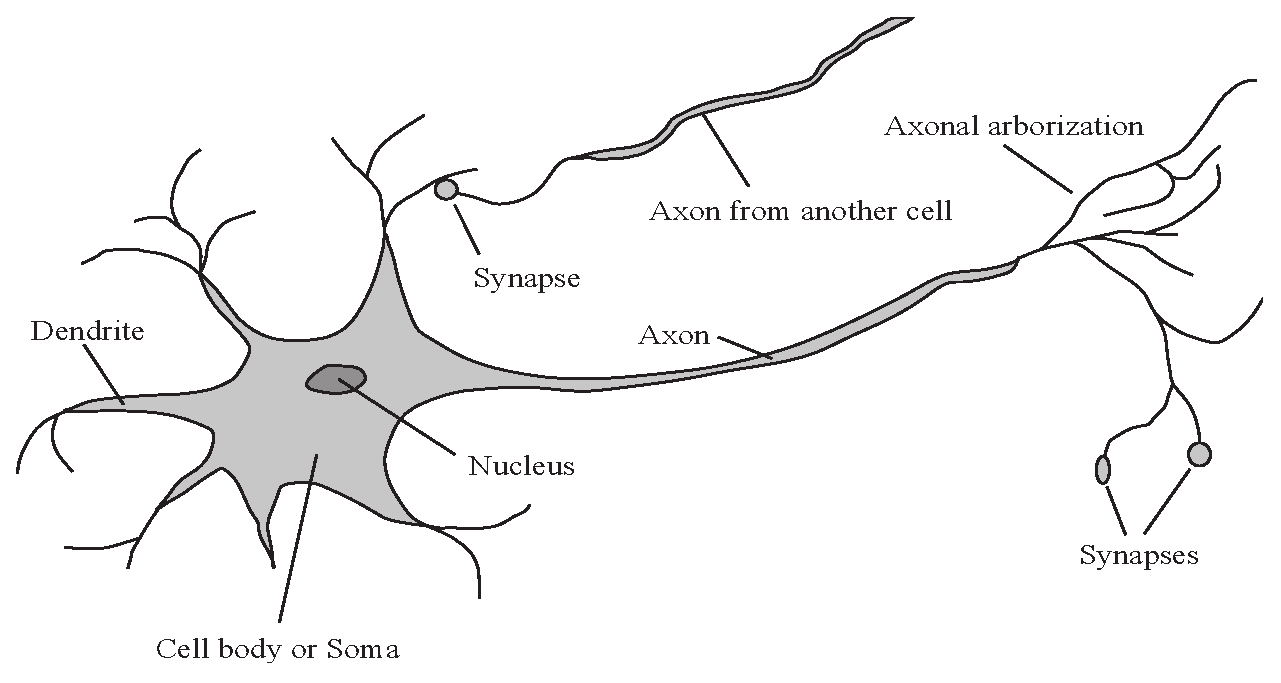
\includegraphics[width=0.95\textwidth]{ModellAvNeuronet.eps}
	\caption{A illustrative model of the neuron. The signal propagation goes from the left to the right in this figure;
			Synaptic integration at the dendrites, action potential through the axon and finally transmission throught the output synapses. 
			The aspects of the cell body is not immediately relevant to signal processing, and is not taken into account in the model used. }
	\label{figFigurAvNeuronet}
\end{figure}

% Gjennomgang, natt til 30juli. Her er eg no.
% TODO TODO TODO TODO TODO TODO TODO TODO TODO TODO TODO TODO TODO TODO TODO TODO TODO TODO TODO TODO TODO TODO TODO TODO TODO TODO TODO TODO TODO TODO TODO TODO TODO 

When the action potential reaches the ``axon terminal'', where the presynaptic membrane of the synapse lies, neurotransmitters are released into the synaptic cleft 
 	(se appendix \ref{appendixSecPresynapticSynapticPartOfTransmission} for a more complete discussion of the action potential and the presynaptic elements of synaptic transmission).
The neurotransmitters diffuse passively out in the synaptic cleft. Some come in contact with the postsynaptic receptors, and activates the receptor.
%The receptors that are relevant to this project is the ligand--gated receptor group.
%Describing the different known kinds of receptors will be outside the scope of this report. We will limit the description to one class of receptors, called ``ligand--gated receptors''.
Directly--gated receptors (also called ``ligand--gated channels'') open a channel when exposed to the right ligand (the right neurotransmittor), 
	causing an increase or decrease in the postsynaptic neurons depolarization\cite{PrinciplesOfNeuralScience4edKAP10}. .
%Ligand--gated receptors are direcly connected to ion channels in the membrane. Opening of these ion specific channels enables some ions to flow throught (depending on what kind of channel the receptor is connected to). 
%Depending on which ions are let through, the neuron is either depolarized (towards zero polarization, less than its resting potential) of hyberpolarized (getting a more negative membrane potential) by the transmission.
Whether the postsynaptic depolarization is increased or decreased by a synaptic transmission defines the synapse as being an excitatory or an inhibitory synapse\cite{PurvesNeuroscienceKAP05}.
%On the postsynapsic membrane in the synapse are different receptors for different neurotransmitters\cite{PrinciplesOfNeuralScience4edKAP10}. 
%The receptors are only activated by some neurotransmitters, and the change in postsynaptic postential varies with what ions the receptor channel is permeable to.

%Since depolarizing the neuron causes firing, the neurons potential is often referred to as the neurons depolarization in the litterature.



\subsection{The Axon and the Action Potential}
\label{ssecTheActionPotential}
In the membrane of the axon we have voltage--gated channels that open if the level of depolarization is more than some value. This value is called the ``firing threshold of the neuron''.
These channels will open and further depolarize the membrane. 
Through passive transmission of the electrical potential, the next voltage gated channels will open as a result of going above the gate threshold. %also go beyond the firing threshold.
This establishes the active aspect of action potential propagation, and results in a self carrying propagating through the axon.
%This establishes the self carrying signal of the axon, and results in an equal depolarization at the different axon terminals\cite{PrinciplesOfNeuralScience4edKAP09}.
An important result of this is that the presynaptic membrane at the synapses recieves an equal depolarization, independent of its location. 
The release of neurotransmitters is a result of this depolarization, and the action potential enshures an equal depolarization of the presynaptic membrane.
This gives that the transmission is dependent only on the synaptic connection, or ``the synaptic weight''\cite{PrinciplesOfNeuralScience4edKAP09}.
%
%This means that sufficient depolarization of the membrane of the axon opens voltage gated ion channels that will further depolarize the membrane. 
%Through passive transmission of the voltage, the signal is distributed to the next voltage gated channels.

%todo skriv mot slutten av paragraf:  The voltage gated channels will only be open for a small period of time.
%There are at multiple kinds of voltage gated channels. The sodium channel opens
For the action potential there are two important voltage--gated channels; The sodium channel and the potassium channel.
The $Na^{1+}$ channel opens faster than the $K^+$, and gives the rising phase of the action potential.
The rising phase of the action potential comes as a consequence of more positively charged $Na^{2+}$ ions outside the neuron causing a strong inward current after opening of the $Na^{2+}$ channels.
Voltage gated $Na^{2+}$ only stay open for about 1 ms before they close.
About the same time as the $Na^{2+}$ channels close, the $K^+$ channels open. 
Because there is a larger concentration of $K^+$ inside the cell, this will cause a more negative potential over the membrane. The neuron is repolarized.
%After some time delay, the $K^+$ channel opens, and at about the same time the $Na^{2+}$--channel close.
%We have more $K^+$ ions inside the cell, so increasing the permeability for $K^+$ will decrease the depolarization over the membrane, or ``repolarize'' the membrane.
%When both channels are closed again we are back at the resting potential of the neuron. %SITER: Bear s:91
After the action potential the membrane potential is ``reset''.
As the electrical potential spead passively to the next site with voltage--gated channels, 
	the refraction period of each voltage gated channel is an impotant mechanism to hinder the action potential from going ``the wrong way''\cite{NeuroscienceExploringTheBrain3edKAP4}\cite{PrinciplesOfNeuralScience4edKAP09}.

To recreate the ionic gradient, the ions are transported back by the sodium--potassiom pump.
As this is a mechanism that use a little time to reset the ionic gradients, we have a little period when the gates have to be closed.
This is the basis for the refraction period of the neuron, a small period of time where action potential cannot be initiated\cite{NeuroscienceExploringTheBrain3edKAP4}.

After firing an action potential, the neuron will also have a short period where it is impossible to exite the cell, called \emph{the absolute refraction period}\cite{PrinciplesOfNeuralScience4edKAP09}.. 
%The refraction period of a neuron usually lasts for a few milliseconds\cite{PrinciplesOfNeuralScience4edKAP09}.
%\cite Bear kap. 4  (s.91, nede) og Kandel kap.9 s 157 (nede)
%TODO TODO TODO TODO TODO TODO TODO TODO TODO TODO TODO TODO TODO TODO TODO TODO TODO TODO TODO TODO TODO TODO TODO TODO TODO TODO TODO TODO TODO TODO TODO TODO TODO TODO TODO TODO TODO TODO TODO TODO TODO TODO TODO TODO 
% Plan: finn referanse på dette, og så sei at eg har matematisk vist det å være sant.
In this project, the author has demonstated matematically that the refraction period is important for limiting the firing frequency of the neuron. 
The analysis is presented in section \ref{ssecValueOfAlpha}.
%In this project the author has formalized that the refraction period is important for limiting the firing frequency of the neuron. The analysis is presented in section \ref{ssecValueOfAlpha}.


%												"close to":  SKRIV OM
The axon is organized as a tree, with a trunk in close proximity to the soma of the neuron, called the axon hillock.
The branches of the ``axonic tree'' are called axon collaterals. 
The elements of the axon that is furthest from the axon hillock is called the axon terminal, and is where the output synapses are located.
%The axon ``ends'' in the axon terminal, where the presynaptic part of the synapse is located.
When the action potential reaches the synapse, a transmission is initialized by the opening of voltage gated $Ca^{2+}$ channels\cite{PrinciplesOfNeuralScience4edKAP10}.
%The signals transmitted in the axon is strictly directional, that is: the signal goes from the axon hillock (close to the neurons soma) to the axon terminals (where the synapses is). 

%ODO Skriv mindre, eller i det minstre mindre kraftige utsagn. Følgande er rett, men kanskje urelevant for denne oppgava?
%You also have modulatory synapses at the axon terminal, that does not contribute to the value of the neuron, only the amount of neurotransmitters released following the next incoming action potential. 
%The modulatory synapse is but an example of the complexity of the simplifications that are neccesary in order to make an artificial neural network.
%In addition we have different time delay for different synapses along the axon, diffuse modulatory systems it the brain with modulatory neurotransmittors, 
%different states as the neurons use the oxigene and nutritients available, etc.






\subsection{The synapse}
\label{ssecTheSynapse}
%\subsubsection{Synaptic Plasticity}
%When the action potential reaches the axon terminal, the size of the signal is thought to be the same as when it first was initialized at the axon hillock.
%This enshures that the distance the action potential has to travel does not affect the transmission at the synapses of the different axon terminals. \cite{NeuroscienceExploringTheBrain3edKAP4}.
Following an action potential, voltage gated $Ca^{2+}$ channels are opened and $Ca^{2+}$ enters the axon terminal.
This causes synaptic vesicles to merge with the presynaptic membrane, causing the content of the synaptic vesicles to be released into the synaptic cleft. %Cite Kandel kap.10
% Forrige to linjer (passer med siste forrige section) ELLER neste linje:
%When an action potential reaches the location of a particular synapse, the membrane potential will cause release of neurotransmittors from the axon terminal (the presynaptic neuron).
%-------------------------------------------------------------------------ordna til hit-------------------------------------------------------------------------------------------------------------------------------------------
The neurotransmitters from the synaptic vesicles diffuse into the synaptic cleft.
If a so--called ligand--gated channel at the postsynaptic membrane is exposed to these neurotransmitters, the channel opens and ions are let thought.
The result is either excitation or inhibition of the postsynaptic node's value, depending on the channel (which ions are let through).
The size of the transmission is based on presynaptic and postsynaptic mechanisms\cite{PurvesNeuroscienceKAP05}.
%The transmission is thought to be a funcion of presynaptic and postsynaptic mechanisms.

\begin{itemize}
	\item Presynaptically, different amount of neurotransmitters can be released from the axon terminal following an action potential.
	\item Postsynaptically, the amount of receptors varies between different synapses. The amount also varies with time. % This is one mechanism of synaptic plasticity.
\end{itemize}

The level of transmission is the background for what is modelled as the synaptic weight in artificial neural networks.
%These two sides of synaptic transmission are important when synaptic plasticity is considered. 
Patterns of long term synaptic plasticity is what is what is percieved as learning in the field of neuroscience \cite{NeuroscienceExploringTheBrain3edKAP25}.
A more comprehensive study of synaptic plasticity is outside the scope of this text, but it should be mentioned that the ion $Ca^{2+}$ is thought important in both presynaptic and postsynaptic plasticity.
The postsynaptic role of $Ca^{2+}$ is important for STDP, which is an important argument for ANN with the capability of calculating the spike time.
%This is important for STDP, which is an important argument for ANN with the capability to calculate the timing of the spike.
For the especially interrested, appendix \ref{appendixSynPlast} considers presynaptic and postsynaptic mechanisms behind synaptic transmission and synaptic platicity, with a special focus on the role of $Ca^{2+}$.








% //{ Kommentert ut.  Gave til meg selv når eg skal skrive masteren (liten gave, nesten ingenting)

% //{
%The conclution from the study about 

% % XX MED-noke-om: For now, it is enough to mention that the synaptic weight changes as a multifactorial function based on 
%For now, it is enough to mention that  $Ca^{2+}$ is important both presynaptically and postsynaptically for synaptic plasticity.
% % We will later make use of some of the 
% % XXX Bra, men passer det inn:
%When the action potential reaches the axon terminal, it will open voltage--gated $Ca^{2+}$ channels in the active zone of the terminal, and $Ca^{2+}$ enters the cytosol of the axon terminal of the presynaptic neuron\cite{PrinciplesOfNeuralScience4edKAP10}.












% The signal arriving at the presynaptic membrane is equal for all the synapses, the transmission is not. 
% The transmission varies as a function of many mechanisms. %xxx Dårlig setning!
% For the scope of this text, we will focus on the mechanisms within the neuron. 
% I will refer to the size of this transmission as the weight of the synapse. 
% % Dårlig skrevet, over her.

%In this report the convention used by Rolls and Treves in ``Neural Networks and Brain Functions'' will be used. 
%For any transmission through a synapse between neuron $j$ and neuron $i$, we define the synaptic strength $w_{ij}$. 
%Note that the first subscript refers to the recieving neuron and the last subscript to the presynaptic neuron (the signalling neuron) \cite{TrevesNeuralNetworks}.
%This convention will be used in this text. 







%This does not mean that the transmission for different synapses is the same. At each synapse the connection to the postsynaptic neuron is different. 
%There are many mechanisms behind this, but I will focus on the mechanisms within the neuron:
% //}

%\subsubsection{Presynaptic mechanisms behind synaptic plasticity}
% //{
%$Ca^{2+}$ causes release of neurotransmittors from the presynaptic axon terminal into the synaptic cleft\cite{PrinciplesOfNeuralScience4edKAP10}. 
%Long--term potentiation (LTP) causes a lasting change of the tranmission through the synapse.% On the shorter time scale we have short--time potentiation, called fascilitation and short--time depression (decrease of transmission) called 
%
%The amount of $Ca^{2+}$ inflow, and thus the amount of neurotransmitter release can be modulated by socalled axoaxonic synapses\cite{NeuroscienceExploringTheBrain3edKAP5}, synapses that is connected directly to the presynaptic axon terminal. 
%A transmission here will cause a small increase in the axon terminals amount of $Ca^{2+}$ and ``prime'' the synapse for a transmission. 
%Multiple incoming action potentials in fast succession will have the same effect on the following action potentials and causes what is called \emph{potentiation} (short term increase in synaptic weight)
%\cite{PrinciplesOfNeuralScience4edKAP14}. 
% %Variation of the $Ca^{2+}$ entering the presynaptic axon terminal, for example by ``priming'' the synapse for transmission by axon-synaptic synapses, is one potential mechanism for synaptic plasticity\cite{PrinciplesOfNeuralScience4edKAP14}.

% X XX Ta vekk mykje av "Presynaptic mechanisms behind synaptic plasticity" om eg ikkje bruker desse effektene i implementasjonen!
% //}


%\subsubsection{Postsynaptic mechanisms behind synaptic plasticity}
% //{
%Glutamate is the main excitatory neurotransmittor in the CNS\cite{PrinciplesOfAnatomyAndPhysiology12edKAP12}. %s. 448
%There are two main groups of ligand--gated glutamate receptors, the N-methyl D-aspartate (NMDA) receptors and the non-NMDA receptors. 
%The non-NMDA receptors mainly consists of the $\alpha$-amino-3-hydroxy-5-methyl-4-isoxazolepropionic acid (AMPA) receptor. %XXX SITER!
%
%Most non-NMDA receptors are permeable to ions that changes the postsynaptic potensial without having lasting changes on the synaptic strength.%efficiancy. 
%The NMDA receptor is permeable to $Ca^{2+}$, which is important for lasting changes of the synaptic strength. %uttrykket 'synaptic strength' har ikkje blitt definert enda. Gjør det lenger oppe. XXX DO IT!
%
%An other important difference between the NMDA-R and the AMPA-R is that NMDA receptors have an additional condition for opening of its ion channel. 
%In the NMDA receptor there is a $Mg^{2+}$ ion blocking the channel. 
%When the potential across the membrane is sufficiently depolarized, the $Mg^{2+}$ will float more freely and the block is removed from the NMDA receptor.
%$Ca^{2+}$ diffuses into the cell following an action potential\cite{PrinciplesOfNeuralScience4edKAP12}.
%
%Also on the postsynaptic part of the synapse $ca^{2+}$ has an important role in synaptic plasticity. 
%$Ca^{2+}$ activates production of more non-NMDA receptors for the postsynaptic membrane, resulting in LTP\cite{AMPARtrafficingArtikkel}.%\cite{PrinciplesOfNeuralScience4edKAP12}.
%
% %TODO Det under gjelder jo bare for kvifor vi får positiv vektendring. Skriv dette, eller finn ut forklaringa for negativ vektendring (LTD) som følge at STDP! XXX
%The NMDA-related synaptic plasticity is the background for what is called ``Spike Timing Dependent Plasticity'' (STDP) that will be important later in this text.
% % XXX ikkje "rest of this text." Det er ikkje viktig over alt. Noken plasser.. Kanskje "an important element in this text."?
% %Skriv om hebbian learning, ustabilitet  og at STDP kalles "stable hebbian learning". Sjå rapport i NEVR3004.
% %STDP has also been called ``stable hebbian learning''. This refers to the 

%\subsection{SKRIV OM STDP! Referer til forrige avsnitt}
% %TODO: sjå rapport NEVR3001, NEVR3003.
% %HER ELLER OVER. kjør \label{forklaringBakSTDP}
% //}

%\label{forklaringBakSTDP} %der forklaringa kommer...

%\subsection{Skriv om Dale's  principle}
%At eit neuron kan sleppe bare en neurotransmittor (eller to, fleire). Desse kan gi ulik virkning på ulike receptore, men i utgangspkt. kan man sei at eit neuron enten er excitatory eller inhibitory. 
%Men dette er også feil. Drøft fram og tilbake.. Skriv konklusjonen (til korleis eg gjør det i min implementasjon) i section{implementation}.


% %Because of the boolean nature of the action potential, the transmission of the action potential to the next neuron is desided by the strength of the synaptic connection.

% %The most studied neurotransmittor is glutamate. In most neurons glutamate is an excitatory 

% %Skriv om STDP (glutamate), om bakgrunnen for STDP: NMDA med mg²⁺ blokk, voltage dependent i tillegg til at utsida må være eksponert for glutamat, Ca²⁺ inflow fører til AMPA-syntese => synaptisk plastisitet! 


%\subsection{nettverket}
% - Med booleanske signal: korleis kan signalet inneholde så mykje informasjon?
% 		- skriv om inter-spike period. Og kanskje om ANN-flyttals variablene som output fra neurona..
% //}



% Før vi kan lage en kunstig variant av neurale system, er det best å modellere det, og bruke matematiske rammer for simuleringa.
% Dette er også for å formalisere det som tidligere er skrevet i "detBiologiskeSystemet". Gjøre mekanismene eksplisitt, matematisk.
\chapter{The Model} 				%XXX KAPITTEL
%TODO Her må er skrive meir om kva modell som er i grunn for SANN, og for den nye modellen. Intro til kapittel.
% Her skal eg skrive om den nye modellen. Kva er \kappa, kva representerer denne, tid går mot uendelig.. osv.

% Disposisjon:
% 
% 1) kva gir depol. for ein neuron. Kva gir input, kva gir lekkasje?
% 2) utledning av depol.-ligning
% 
% 	TODO Lag frampeik om at "dette kan brukes til ANN", eller tilsvarende.
%

\section{Mathematical modelling of the biological neuron} 
\label{secMatematiskModelleringAvBioNeuron}

%Når eg skriver om:
% Fokuser mest på at value, dvs. depol. til neuronet er kva som er viktig i forhold til fyring av AP. Difor bør vi prøve å modellere dette.
% Ikkje tenk på Nernst, her. Det kommer i neste avsnitt.

Mathematical modelling of the neuron helps understand the neuron, and the mechansims behind how the neuron works.
A good model of the neuron will also give us a guide when simulating the system.

In the neuron, the value of each node is given by the electrochemical potential over the cell membrane. 
The neuron will fire an action potential if the value goes over the firing threhold. This makes the value of the neuron an important aspect of neuronal signal processing.
When a neuron recieves a synaptic transmission, ligand--gated channels are opened, and the potential of the neuron is changed as a function of the time the channel is open, and the electrochemical driving force for the charged molechules.
One part of the driving force is given by the electrical potential over the membrane. % XXX vent med dette : When ions are allowed to flow through a channel, the amount that will flow is given
The electrical potential can be seen as a potential field for charged particles.
An other element of the driving force is the distribution of the indivitual ions. Ions are transmitted across the membrane by passive diffusion. 
This meens that the indiviual ions are pushed down its concentration gradient.
If we combine these two effects we get a simplified system of the neuron.
%TODO REFERER: \ref{NeuroscienceExploringTheBrain3edKAP3}
%TODO TODO Skriv om! Bare rot!

% TODO Slett det under. Skriv alt heilt om!
In the biological neuron, the value of the node is governed by many factors. 
The individual ion's equilibrium potential can be calculated by the Nernst equation (eq. \ref{eqNernstEquation}).
%TODO Vent med dette:    For the artificial neuron the value corresponds to the membrane potential of the biological neuron.


The membrane potential of the biological neuron is given by the distribution of electrically charged particles and molecules over the  membrane.
The electrical potential is an impoirtant part of the driving force for changing the value of the node.
From this we can later talk about the differential equation of the nodes value.
%These are two of the mechanisms that gives the 
%The electrical driving force is not the only one, and the value of the node at equilibrium is given by the sum of all these driving forces.
%An important equation in this respect is the Nernst equation.


% TODO TODO TODO TODO TODO TODO TODO TODO TODO TODO TODO TODO TODO TODO TODO TODO TODO TODO TODO TODO TODO TODO TODO TODO TODO TODO TODO TODO TODO TODO TODO TODO TODO 
% Skriv også at simulering er basert på modellering, og at bedre modellering gir oss inspirasjon til nye typer simuleringer. (sikt veldig til meg, uten å sei det..)
% Det fører også til bedre simuleringer?



\subsection{The equilibrium potential}
% TODO TODO Skriv også om lekkasje! Fra ANN.tex refererer eg hit når eg snakker om lekkasje. XXX Hugs å skrive om lekkasje her!
% Sjå ANN.tex: Snakker om LIF-neuron. Skriv om LIF-neuron når eg skriver om lekkasjen!
\label{ssecTheEquilibriumPotential}
%TODO Er det her eg skal skrive om LIF-neuron (leaky integration)?
In the biological neuron, the reversal potential for the different ions is can be calculated by the Nernst equation. 
The reversal potential is the electrical potential where the respective ion flow will be revesed (flow the oposite direction) if an ion channel is opened.
This also involves that at the reversal potential, we get no ionic current following a channel opening. 
This is due to a balance between the driving force provided by the concentration gradient of the ion and the electrical driving force.
The reversal potential is also called the equilibrium potential.
%The reversal potential is the potential where opening of the ions channel causes no net current flow through the membrane.

% XXX Skrive inn nernst-equation? Referer kapittel 3 i Bear. (s 65)
\begin{equation}
	\label{eqNernstEquation}
 	E_{ion} = \frac{C}{z} log\frac{[ion]_o}{[ion]_i}
\end{equation}
Where $E_{ion}$ is the equilibrium potential for the ion, C is a constant (for some temperature), z is the charge of the ion and $[ion_i]$,$[ion_o]$ gives the number of ions on the inside and outside of the membrane
\cite{NeuroscienceExploringTheBrain3edKAP3}.

For a neuron permeable to a single ion, the equilibrium potential will be the same as this ion's equilibrium potential. %ref kandel kap 7. s129
For systems where permeability of multiple ions are involved, the equations for each ion becomes a sum of electrical driving force and chemical driving force multiplied with membrane conductance for the ion
\cite{PrinciplesOfNeuralScience4edKAP07}.
%skrive om at dette gir oss at for en komplett simulering av dette, trenger vi en variabel som holder orden på kvart ion.
A good simulation of the system therefore should have one variable for each of the electrically charged particles and molechules.
There are many important ions and also a couple of protheins and neurotransmittors that are electrically charged, so this will introduce a large computational load in the simulation.
%Many, if not all of the previous implementations I have seen have a simplified structure for the node's value, by having one activation value; The electrical potential.
To my knowledge, no implementation of SANN with a pragmatic use (i.e. used in technology) uses multiple ions to find the depolarization of the nodes in the simulation.
These implementations use the electrical potential as the value for each node. This will also be the focus of the remaining part of the modelling section.
%It is unknown wheter this removes any important aspects of the neuron.

% Todo: Skriv om neste linja!
At rest, the membrane is permeable to some ions, and to prevent the ion reaching (and staying) at the neurons equilibrium potential, there are active pumps maintaining a different potential. 
%
In the postsynaptic membrane of some synapses there is so--called \emph{ligand--gated ion channels}, channels that are activated by exposing the activating neurotransmittor\cite{NeuroscienceExploringTheBrain3edKAP5}.
The channel will be open for a small time period, causing a flow of the ions that are let throught the channel, giving an altered postsynaptic potential. 
Excitatory synapses increase the postsynaptic node's value. This is called an Excitatory PostSysnaptic Potential --- E-PSP \ref{PrinciplesOfNeuralScience4edKAP07}.

Other ligand--gated channels have other channels that will decrease the value of the neuron.
%Inhibitory synapses have other channels that causes an inhibition of the postsynaptic neuron. 
Because this inhibits the neuron in respect to firing an action potential, this is called inhibitory synapses, and the postsynaptic effect of a transmission is called Inhibitory PostSynaptic Potential (I--PSP).
%This involves decreasing the postsynaptic neurons value. This is called an Inhibitory PostSynaptic Potential (I-PSP).
%XXX ref kap 7. kandel.
Because of time limitations, modelling of the time delay and size of each transmission has not been evaluated in this project.
An other aspect that will be for further research, is modelling and implementation of synaptic plasticity. 
This is one important reason behind using artificial neural networks in technology, and the reason behind developing the spiking variant of ANN.
Synaptic plasticity will hopefully be modelled and implemented in a later project.
%This project is about the comparison between 

%Opening of a membrane channel will change the permeability of the membrane to some ions (depending on the channel), and the ion pumps will not be able to maintain the potential different from the equilibrium potential. 
%This causes the potential of the neuron to change accordingly, and is the basis of exitatory and inhibitory postsynaptic potentials (E-PSP/I-PSP)\cite{PrinciplesOfNeuralScience4edKAP07}.
%X XX ref kap 7. kandel. s. 131




Some of the aspects in the theory of the electrical potential for the neuron was introduced to show that the simulated system is a complex one, even at the level of the individual node. %Videre har vi også at proteiner kan ha ladning.
For each node we have a complex system with a continously changing driving force and membrane conductance for each ion. 
For artificial neurons used in an ANN most of these aspects can be simplified without affecting the result much. 
Because the primary focus for this implementation is the use of the neural simulator in technology, the efficiancy of the implementation is crucial. 
We therefore have a single variable giving the membrane potential as the activity variable in this implementation. 
The extra computational load introduced by multible activity variables is not worth is for simulators with a pragmatic focus. %Kva meines med pragmatic focus? Skriv dette..
%TODO SJå over avsnittet og få bedre flyt!
%In addition this is the VANLIGE INNEN SANN.

%It is also important to know about the complex structure of neural signal processing


%Rensa opp litt til hit. *********** fortsett rensing herifra. ****************


%skriv om neste:
%The reason for introducing the background information about the neuron is  %TODO SKRIV OM: Skriv at det er viktig for å forstå simulatoren min(meir om dette seinere). XXX Ta vekk denne itemize(?):
%\begin{itemize}
%	\item to introduce the ide of different states for the neurons membrane. Each with its own equilibrium potential.
%	\item to introduce an important consept for the neuron that will be important for ANN as well, $V_{r}$.
%	\item to describe the complexity of the system. For a complete simulation of a neuron, each ions distribution across the membrane may need to be simulated as a dynamical system.
%	\item to give the background for the system to be modelled as a leaky integrator. The neurons value ``leaks'' toward the equilibrium potential.
%\end{itemize}














\subsection{------------SKREVET OM TIL HIT.----------}





$V_{r}$ will be used as the resting membranes potential. For biological neurons this can be calculated by the Goldman equation\cite{PrinciplesOfNeuralScience4edKAP07}. 
For our use if will be enough to know the extistance of the equilibrium potential for a membrane at rest,
in addition to define a resting membrane potential for the implementation of the artificial neuron.

%For multi--ion systems modelling the system becomes more complicated, but for our use it is enough to know that there is a resting membrane potential that is a function of


% TODO Minimaliser reperering av det er nettop har sagt.. XXX

%It is important however to know that there is such an equilibrium potential, given by the sum off all the contributions (from the individual ions).

Because of the active pumps, different states with different permeability do the different ions will give different membrane potential because of different factors for each part of the ion differential equation. 
The membrane at rest, that is with no open ion channels, gives the resting membrane potential, $V_r$. 

In the case of synaptic input to a neuron, the postsynaptic membrane will open ligand gated channels (se section \ref{ssecTheNeuron}). 
Both for exitatory and inhibitory input this will push the neurons value and could be seen as an external force in the system.
%For our use, we set this external force to be a constant.
Whether this external driving force can be percieved as a constant or is a more complicated dynamical system is as everything else in the nature; complicated. %Skriv slutten analeis.
The neuron has NMDA channels that are more permeable to both the normal ions in addition to $Ca^{2+}$. Since the NMDA-R is voltage dependent, this causes the glutamatic transmission to be a function of the postsynaptic potential.

%For E input. Kva skjer. Sjå på som eksternt pådrag. 
As this is a mechanism that is little described in articles in neuroscience and to my knowledge not used in ANNs, I will not use voltage dependent exitatory ion channels in my two implementations of ANN. 
%Skriv at dette uansett ikkje har noko innverkning på resultatet? Eller blir dette også dumt i forhold til relevansen til denne linja i teksten?
For my implementations the external driving force on the membrane potential will in other words be a constant.

%Skriv om lekkasje. Forbered på neste seksjon.
%When the potential over the membrane does not equal this equilibrium potential, the system will be driven toward this equilibrium. %(without any external input).

%In the case of neural networks, this is called a 'leaky integrate-and-fire' (LIF) model.

%TODO Poengter at dette er mitt arbeid:
\subsection{The differential equation for neurons depolarization} % (gjør om chap til sec. ,no. Skal denne bli subsubsection?
The equation for the potential can be stated as a first order differential equation:
\begin{equation}
	\dot{v}(t) = \dot{v}_{in}(t) - \dot{v}_{out}(t) %, \qquad i = \text{ neural input } %% XXX Endra \dot{v}_{in}(I) til  \dot{v}_{in}(t). XXX
	% skriv også at det er \dot{v}_{out]}(t, v(t)) ---avhengig av v(t) også!
\end{equation}
Where $\dot{v}_{in}(t)$ gives the effect of synaptic input to the neuron% XXX KVA er PÅDRAG på engelsk?
	, and $\dot{v}_{out}(t)$ represents the ``leakage'' of the neurons value.



% TODO Ikkje del opp i underavsnitt: Skriv heller "Element for diffligninga", eller noke, og få med begge her.
% Men det eg heller kan ha med som underavsnitt er "forkrav for ligningene" eller "utgangspkt" eller "antagelser for ligningene"...
\subsubsection{The input}
The input, represented by $\dot{v}_{in}(i)$ in the above equation, is a function of the neurons exitatory and inbibitory input. 
The neurons input waries with time, but for now we look at the variable $I$ as a constant in respect to time.
%One method for a varying degree of input will be introduced in section \ref{ssecVariableInputBetweenSpikes}.
Later, in section \ref{ssecVariableInputBetweenSpikes}, the method will be expanded to account for a varying degree of input. % (section \ref{ssecVariableInputBetweenSpikes}).

\begin{equation}
	\dot{v}_{in}(t) = I
\end{equation}
%$I$ is the effect of the input to the neuron (sum of exitatory and inhibitory input).
$I$ represents the effect of the synaptic input to the neuron at time $t$, the sum of the effect of exitatory and inhibitory input to the neuron.

%skriv også at v_in(i) er i virkeligheita eit dynamisk forløp, men for ANN kan vi forenkle, og sjå på denne som konstant.


\subsubsection{The ``leakage''}
%TODO Finn referanse for neste påstand!
The neuron is often modelled as a leaky integrator. The ``leakage'' is dependent on the polarization over the membrane. 

For biological neurons, the leakage is given as a function of the difference between the membrane potential and the resting membrane potential $V_r$. 
If we define the resting membrane potential for our artificial neuron to be zero, the leakage will vary propotionally to its potential $v(t)$.

%For artificial neurons, we can set this equilibrium potential to zero %for letthetens skuld. Kva blir dette på engelsk?
\begin{equation}
	\dot{v}_{out}(t) = \alpha v(t)
\end{equation}

In a biological neuron, the propotionallity constant, $\alpha$ is given by the distribution of different ion channels active at rest, the extracellular ionic environment compared to the intracellular level of the different ions, etc.
For our basic ANN this will be cept constant. For more advanced versions of this simulator, $\alpha$ could vary as a function of the intracellular ion--levels. 
In addition we have that the extracellular ionic environment is to large extent maintained by glial cells.
%In the CNS you have so--called astricytic domains governed by astrocytes (a certain kind of glial cell). In this domain the 
% BRIFEKUNNSKAP:XXX :  In the CNS you also have socalled astrocytic domains, where the support--cells for the neurons have domains. Inside this domain one astrocyte is 


\subsection{The depolarization equation}%equation for the neurons value}
This gives us the differential equation 
\begin{equation}
	\dot{v}(t) = \dot{v}_{in}(I) - \dot{v}_{out}(t) = I - \alpha v(t)
\end{equation}

Laplace transformation gives
% XXX Legg utledning av uttrykk i appendix! 		Her skal bare stå: V(s) = ...
\begin{equation}
	\begin{split}
		sV(s)-v_0 		&= \frac{I}{s} - \alpha V(s) 			\qquad, \; \qquad v_0 = v(t_0) 				\\
		(s+\alpha)V(s) 	&= \frac{I}{s} + v_0 														\\
		V(s) 			&= \frac{1}{s+\alpha}\left( \frac{I}{s} + v_0 \right)
	\end{split}
\end{equation}

And 
% XXX Legg utledning av uttrykk i appendix! 		Her skal bare stå: V(t) = ...  XXX type: bare siste linja i den kompilerte DVI'en
\begin{equation}
	\begin{split}
		v(t)  	&= 		\mathscr{L}^{-1}\bigg\{ V(s) \bigg\}  									\\
		 		&=		\frac{I}{\alpha} - \frac{I}{\alpha} e^{-\alpha t} + v_0 e^{-\alpha t} 	\\
				&= 		\kappa \left( 1 - e^{-\alpha t} \right) + v_0 e^{-\alpha t} 	\quad,\; \kappa = \frac{I}{\alpha} 
		\label{eqVerdiligninga}
	\end{split}
\end{equation}

The diversity of neurons makes it unrealistic to generalize over all neurons, and say to what the value is reset to.
For our artificial neuron we can define 
%Generalization for all neurons is unrealistic due to the divesity of neurons, but for our synthetic neurons we can define
that the neuron is reset to what corresponds to the equilibrium potential at rest, $V_r = 0$ after firing an AP.
%In the simulated neurons this means that after firing, the neuron is reset to $v_0=0$ after firing. 

The action potential is a discontinuity in the othervise continous system. The continous equation is only valid between action potentials (within one period).
%If we reset every aspect of the equation to be reset after firing, the equation can be used for the discontinous system. 
To use \eqref{eqVerdiligninga} for the whole time range, we define $t = t_{abs}-t_f$, where $t_{abs}$ is the absolute time and $t_f$ is the time of the last action potential. 
In this way $t$ represents the time since the start of the current period.

%If we define a time window as the time interval between time of reset (after firing) to next firing, we can define time $t$ as time after start of time window. This defines the time of reset as $t=0$.
%We define the time of reset as $t=0$.


%Equation \eqref{eqVerdiligninga} describes a continous nonlinear system. 
%In the neuron we have that if the neurons value goes above some threshold the neuron will fire an action potential, and the value is reset. This introduces yet another nonlinearity: 
%The action potential.

\subsection{The Action Potential}
The action potential, a ``spike'', and the period between action potentials, the interspike period, is the basis of the computational capabilities of the neuron.
When the value of the neuron excedes the firing threshold an action potential is initialized.
This causes transmission at all the output synapses of the neuron, and resetting the value of the neuron to $V_r$. % = 0. Skrive at det er lik null. Gjør likningene under rett..

We get that the neuron fires at time $t^*$:
\begin{equation}
	\begin{split}
			v(t^*) 					 							&= \tau \qquad 										\\	%,\qquad\qquad\tau = \text{firing threshold} 	\\
			\kappa (1-e^{-\alpha t^*}) + v_0 e^{-\alpha t})		&= \tau 											\\
	%		(v_0-\kappa)e^{-\alpha t^*}							&= \tau-\kappa 										\\
			\ln \left(e^{-\alpha t^*}\right) 					&= \frac{\kappa - \tau}{\kappa - v_0} 					\\
			t^*													&= -\alpha^{-1} \, \ln \left( \frac{\kappa - \tau}{\kappa - v_0} \right) 					
	\end{split}
	\label{eqTidTilFyringVedEndraKappa}
\end{equation}

Where $\tau$ is the firing threshold of the neuron. 
%XXX TODO Neste linjene er litt feil. Dette beskrive oppladninga av depol., m.a.o. ikkje heile p_isi(K). Bare p_charge,isi(K). Skriv dette. 
% ( Skriv at i tillegg får vi den såkalla "refraction time" errer eit AP. Dette må legges til for å få heile perioden.
If we define $p_d(\kappa)$ as the depolarizing phase of the inter--spike interval, for constant inter--spike $\kappa$ we get $v_0 = 0$, and the depolarization phase of the period is given by
\begin{equation}
	p_d(\kappa) = -\alpha^{-1} \, \ln(\frac{\kappa - \tau}{\kappa})
	\label{eqPeriodeligningForKonstIntraPeriodKAPPA}
\end{equation}

Equation \eqref{eqTidTilFyringVedEndraKappa} can also be used to calculate the time until firing for a given $\kappa$ and start value $v_0$
\begin{equation}
%	\begin{split}
	p_{r}(\kappa, v_0) 	\;= t^* + t_r 
						\quad= -\alpha^{-1} \, \ln \left( \frac{\kappa - \tau}{\kappa - v_0} \right) + t_r
%	\end{split}
	\label{eqRemainderOfPeriod}
\end{equation}
Here $p_r(\kappa, v_0)$ represents the remainder of the current inter--spike period and $t_r$ the absolute refraction period. % TODO XXX Skrive om dette? :  To see the refration time as a constant is a simplification.
The refraction period is more complex than so, but for our simple model we use this model of the refraction period.

It is impotant to remember that equation \eqref{eqPeriodeligningForKonstIntraPeriodKAPPA} and \eqref{eqRemainderOfPeriod} is based on a constant $\kappa$ during the whole period. 
% Det er meir komplisert enn det som står på neste linje. (gjør det litt større).
If $\kappa$ varies during the interspike period, the firing time will also change. %More on this in the next section.

%If $\kappa$ varies during the interspike period, $t^*$ from equation \eqref{eqTidTilFyringVedEndraKappa} is an estimate of the remainting time until firing. This estimate is updated every time $\kappa$ is.

%TODO Lag ei ligning for heile perioden også? Dette er bra å referere til!



\subsection{Variable input between spikes}
% TODO Skriv heilt om!
\label{ssecVariableInputBetweenSpikes}
Equation \eqref{eqPeriodeligningForKonstIntraPeriodKAPPA} is based on a constant $\kappa$ during the inter--spike period.
% TODO Skriv om neste poeng: kom inn på ideen / beskriv ideen om "time window".
%If we use this equation as the activation function of the node, we still can find the timing of the nodes action potential. STEMMER BARE DERSOM  if $\kappa$ is kept constant during the time interval.

%If $\kappa$ needs to be constant during the whole period, we get a large time lag for the system, so we need to devise a scheme for avoiding this.

If we allow the activation level of the node to change during the inter--spike period of the neuron, we cannot use \eqref{eqVerdiligninga} and \eqref{eqTidTilFyringVedEndraKappa} directly.
																			%the equations from the previous section.
To solve this problem, the concept of a ``time window'' is introduced. A time window is defined as the smallest of [a time interval where the activation level of the node is constant] or [the remainder of the interspike period].
%Within each time window both \eqref{eqVerdiligninga} and \eqref{eqRemainderOfPeriod} is therefore valid. % .. kan bli brukt.
Both equation \eqref{eqVerdiligninga} and \eqref{eqRemainderOfPeriod} is therefore valid within a time window.

\begin{figure}[hbt!p]
	\centering
	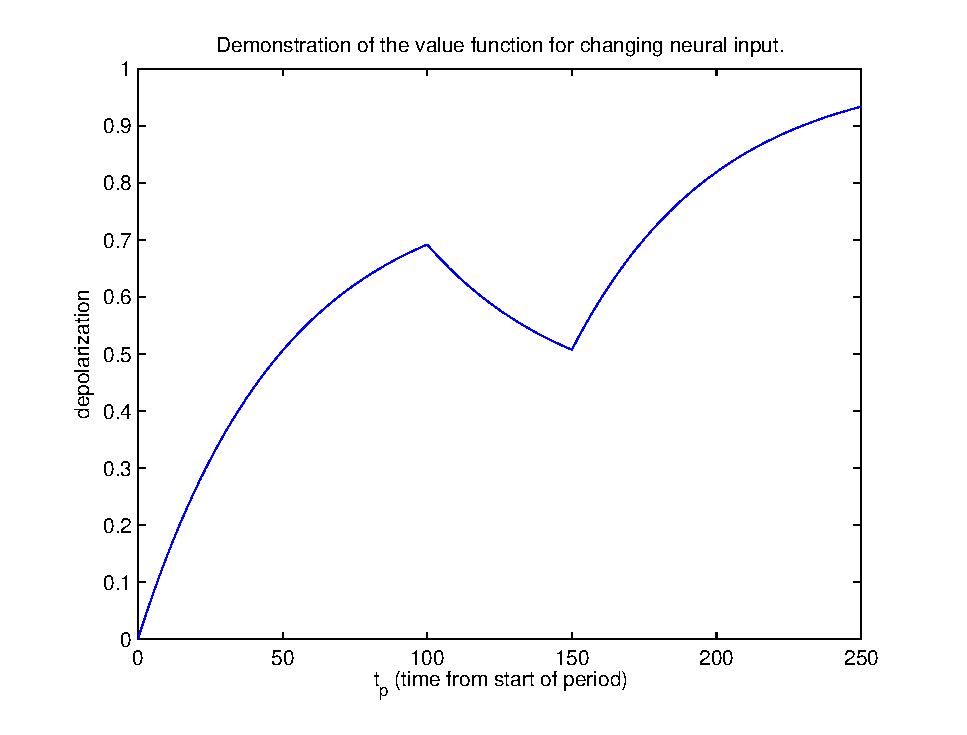
\includegraphics[width=0.95\textwidth]{demonstrasjonAvUlikeKappaforVerdifunksjonen.eps}
	\caption{$v(t)$ for changing $\kappa$. $\kappa_0=0.7$. At time $t_p=100$ $\kappa$ changes to $\kappa_1=0.5$. At time $t_p=150$ the neurons imput increases, and $\kappa$ becomes $\kappa_2=1$. See eq.\eqref{eqVerdiligninga}.}
	\label{figVerdifunksjonen}
\end{figure}

When $\kappa$ is changed, the initial value of the next time window, $v_0$, can be calculated from \eqref{eqVerdiligninga}. 
We can now use \eqref{eqTidTilFyringVedEndraKappa} to find the new estimate for the firing time of the node.
I use the word estimate because we can not know when $\kappa$ will change.
If $\kappa$ is changed before the estimated firing time, the firing time will be affected. 
%XXX if this is before the estimated firing time, the estimate of the next task time will change accordingly.  %If $\kappa$ is changed, the estimate changes.
%-> da er det "but an estimate of firing time.."

%Equation \eqref{eqTidTilFyringVedEndraKappa} gives us the time of firing for a situation where the initial value of the node can be different from zero.
%Also this equation is based on a constant $\kappa$.





%The equations can also be used as the non--linear activation function for a fANN. This activation function is based on a mechanistic model of the biological neuron.
%The activity can be read out of eq. \eqref{eqPeriodeligningForKonstIntraPeriodKAPPA} as the frequency $f(t) = \frac{1}{p(\kappa)}$
%
%If we let the activity level vary between spikes, the model will give as accurate timing as ``Spiking Artificial Neural Network''(SANN). We will discuss different aspects of artificial neural networks later. %XXX Ref?
%The model is based on fundamentally different equations than the model for SANN. 
%If this new model is as effective or more effective than SANN this project will be a contribution because we calculated the firing time in a new way.
%%Ta vekk siste, forrige linje?

%An other aspect with this new model is that it lies between the two prior models of ANN, and can easily communicate with both.

% If we allow the input and activity of each neuron to vary between spikes, the model approaches the model for the biological neuron.
% When $\kappa$ is updated, a new time window starts. 
% $v_0$ from \eqref{eqVerdiligninga} now represents the value at the start of the time window ( $v_0 = v(t=0)$ ). 
% This value is equal to the value $v(t)$ at the time of change of $\kappa$ from the previous time window(se fig. \ref{figVerdifunksjonen}).
% This is equal to the value of the neuron at the time of variation of $\kappa$ (the value at the end of the previous time window).

In fig. \ref{figVerdifunksjonen}, $v(t)$ is simulated for three different time windows. At time $t_p=100$, $\kappa$ changes from $\kappa_0=0.7$ to $\kappa_1=0.5$. At time $t_p=150$, $\kappa$ becomes $\kappa_2=1$. 
The simulation implies that the value function is a continous function that converges toward the neurons final value, $\kappa$, also when $\kappa$ varies.


With this new use of eq. \eqref{eqVerdiligninga}, we can calculate the remaining part of the neurons period after $\kappa$ changes value. 
The remaining time of the period is given by equation \eqref{eqTidTilFyringVedEndraKappa}, given constant $\kappa$. 
If this is updated each time $\kappa$ varies, we get an estimate of the remaining time based on the present $\kappa$.

%Skrive at dette plottet IKKJE er fra kjøring av programmet?




%TODO Finn eit bedre navn på denne subsubsection.
\subsection{The constants in the depolarization equation}
%\subsection{Redying the equation for use in ANN}
%TODO Skriv at denne ligninga kan brukes direkte for å lage en heilt ny modell for "spiking ANN" (ANN med information om 'spike-time').
% 	Om dette skal gjøres, må modellen tilpasses. Blabla, dette gjøres her. Eller noke.. Kanskje ikkje.
\label{ssecValueOfAlpha}

%TODO TODO TODO TODO TODO TODO 
% Skriv om 'value of alpha'! 	TODO TODO TODO TODO TODO TODO TODO 
%TODO TODO TODO TODO TODO TODO 

%XXX Veit ikkje om dette er relevant!

The inter--spike interval for a neuron consists of two phases. 
The absolute refraction period and the depolarizing phase (se sec. \ref{ssecTheActionPotential}).

Equation \eqref{eqPeriodeligningForKonstIntraPeriodKAPPA} describes the depolarizing phase of the neuron. % , $p_d(\kappa)$.
The equation for the whole inter--spike interval is given by
\begin{equation}
	p_{isi}(\kappa) = p_d(\kappa) + t_r
	\label{eqHeilePerioden}
\end{equation}

Where $t_r$ is the absolute refraction period of the neuron. % , and $p_d(\kappa)$ is given in \eqref{eqPeriodeligningForKonstIntraPeriodKAPPA}.
If we consider the firing frequency of the neuron, $f(\kappa) = p_{isi}^{-1}(\kappa)$ we can se that the asymptote is given by
\begin{equation}
	\begin{split}
		\lim_{\kappa->\infty}{ f(\kappa)} &= \lim_{\kappa->\inf}\left( \frac{-\alpha}{\ln \left( \frac{\kappa - \tau}{\kappa} \right) - \alpha t_r} \right)   \qquad = \frac{1}{t_r} \\ 
		%\lim_{\kappa->\infty}{ f(\kappa)} &= \frac{1}{t_r}
	\end{split}
\end{equation}

%Using l'Hôpital's rule %INNI ln(-) funksjonen. TODO Viktig å få med dette i denne setninga!
%and get %sjå wolframalpha.com ...
%\begin{equation}
%	\label{eqFrekvensLlim}
%	\lim_{\kappa->\infty}{ f(\kappa}) = \frac{1}{t_r}
%\end{equation}



We can see from this analysis that the refraction period of the neuron is fundamental for restricting the neurons output frequency (se fig. \ref{figFrekvensMedOgUtenRefractionPeriod}).
For biological neurons, the maximum firing frequency is about 1000 Hz \cite{NeuroscienceExploringTheBrain3edKAP4}. %s 79
\begin{equation}
	\lim_{\kappa->\infty}{ f(\kappa}) \approx 1000 \, \text{Hz}
\end{equation}
%If we define the maximum firing frequency to be 1000, equation \ref{eqFrekvensLlim} gives us the absolute refraction period as
We define the maximum firing frequency for the artificial neuron to be 1000 Hz. From equation \ref{eqFrekvensLlim} we get the absolute refraction period as
\begin{equation}
	t_r = \frac{1}{1000 \text{Hz}} = 1 \, \text{m}s %= 0.001 s = 
\end{equation}

%TODO Skriv at dette er en kjendt størrelse i neuroscience (finn, referer), og er en indikasjon på rettheten til lingningene (?)
% 		Kanskje også skrive litt om at dette er "absolute refraction period". Det er også en mild refraction period etter dette (finn,referer). Dette kan implementeres ved 2ms refraction period for auronet. 
% 		TODO TODO Sjekk andre linja her, og gjør en bestemmelse i forhold til mine ANN. (1 eller 2 ms refraction period?).
If we define the time step of the simulation to be 1 m$s$, the refraction period will be one time step in the simulation.
With a time step of 1 m$s$, the absolute refraction period (the time interval where it is impossible to exite the neuron) can be set to one time step. 
For SANN nodes, this means that the node will not change its value for the duration of the next time step. 
For $\kappa$ANN this can be implemented more effective by incrementing the estimated firing time by one time iteration. 
%TODO fullfør!


% Plott av frekvens med, og uten refraction period:
\begin{figure}[bhtp]
	\label{figFrekvensMedOgUtenRefractionPeriod}
	\begin{center}
		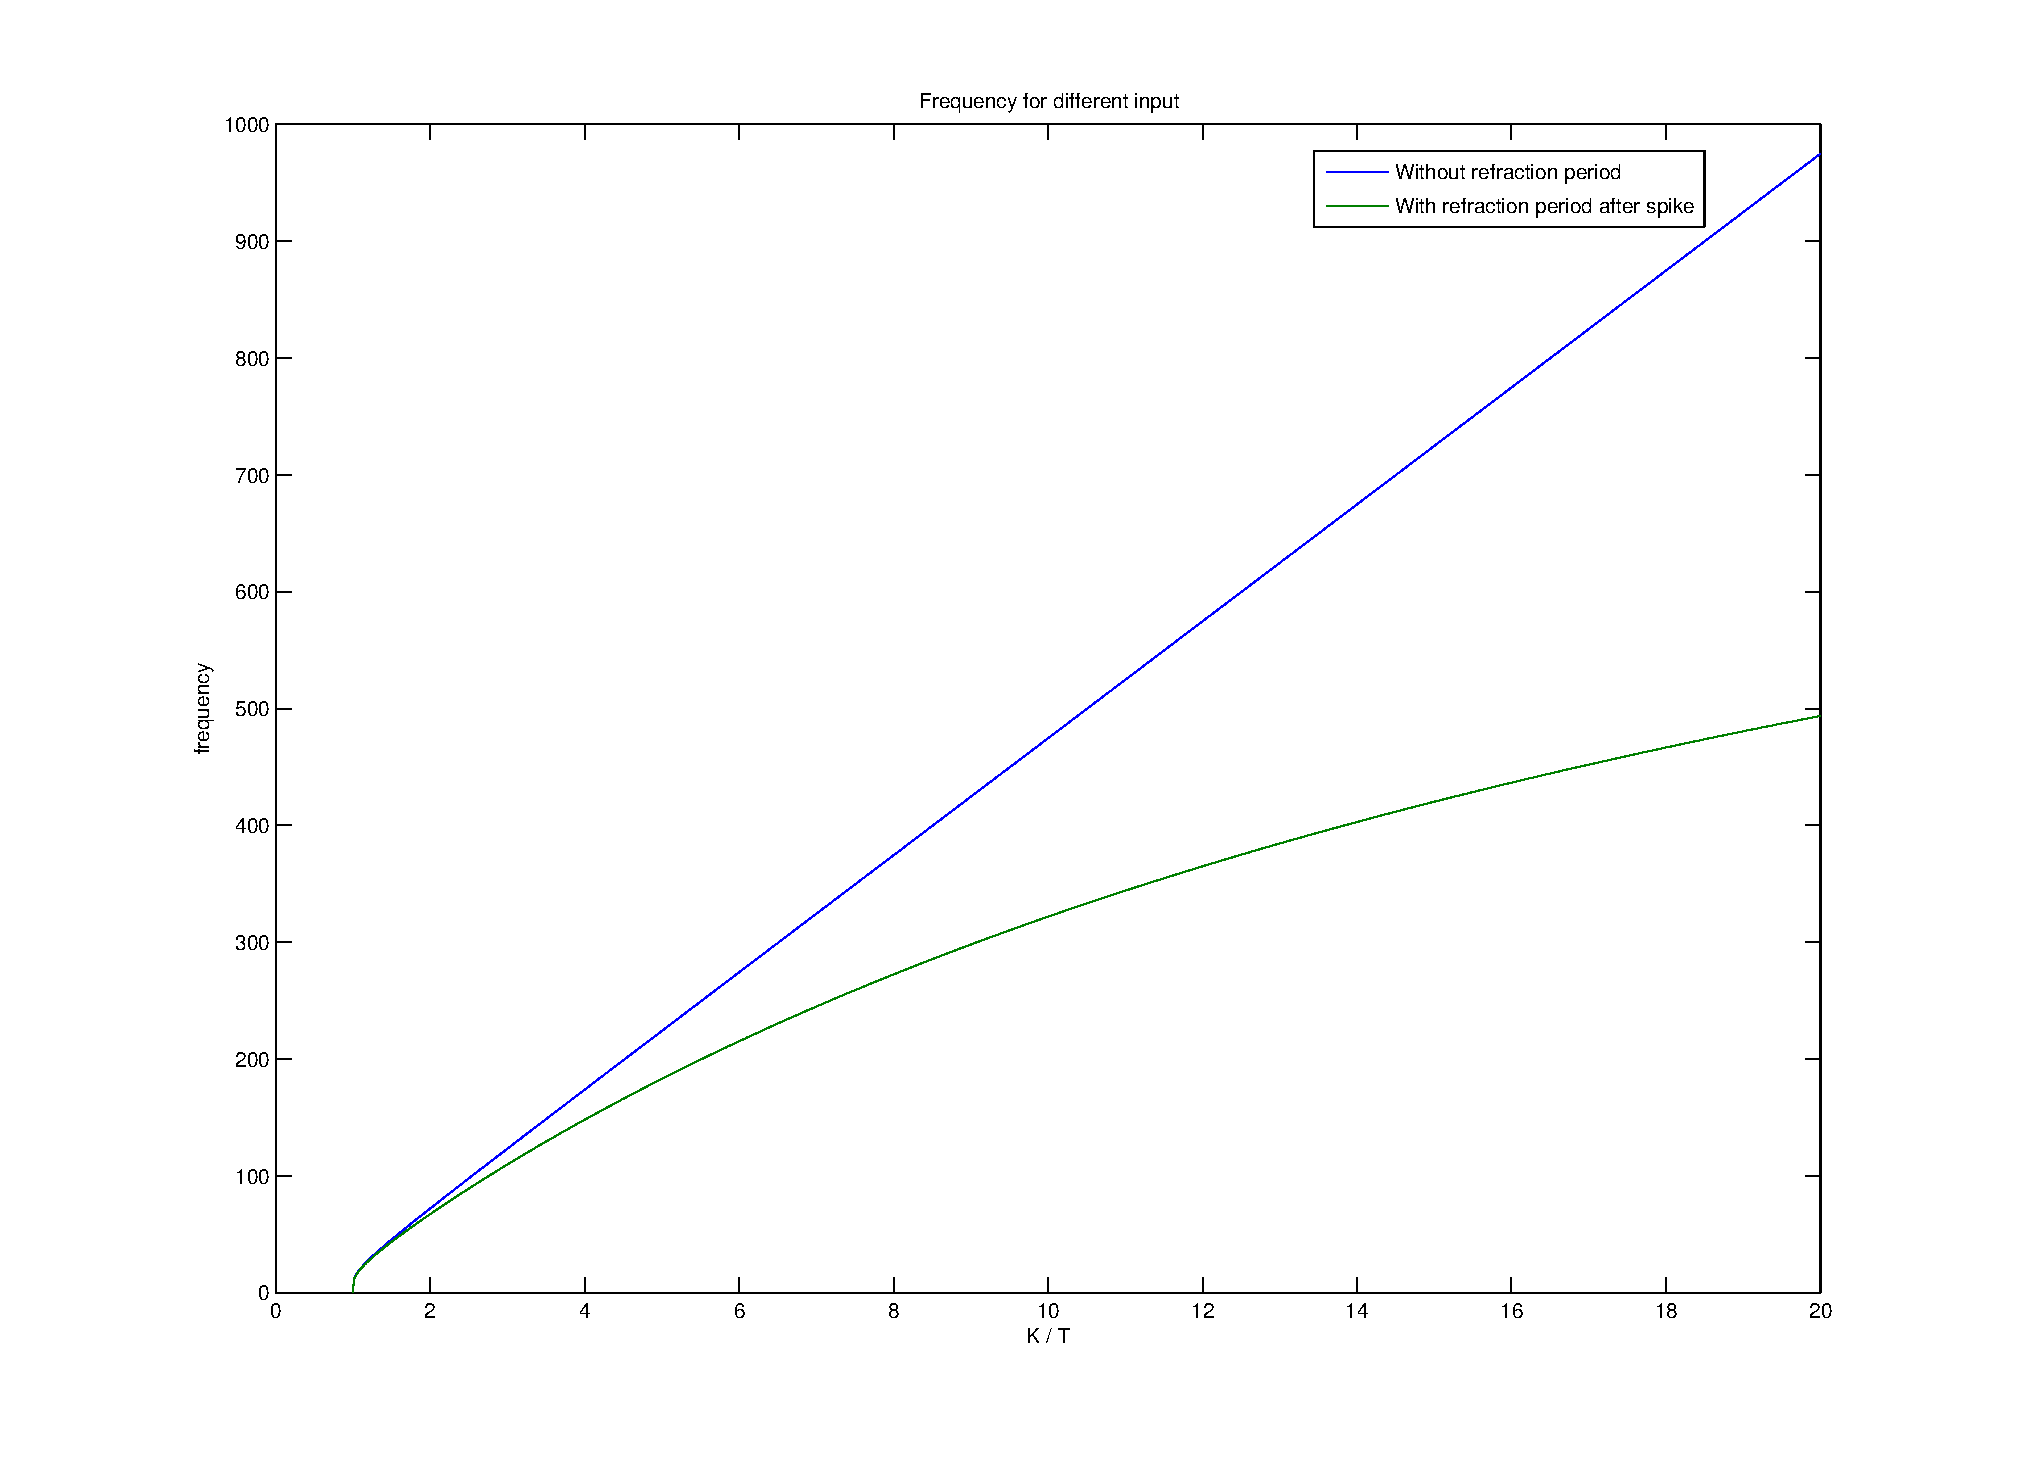
\includegraphics[width=0.95\textwidth]{frekvensPlotRefractionPeriod.eps}
	\end{center}
	\caption{Frequency for a neuron for different values of input. With and without refraction period}
\end{figure}



%TODO Skriv meir om kva de ulike variablane betyr. Kva er \kappa! kva er \tau,\alpha. Skriv om v_0 for tidsvinduet (referer mykje til rett section)



%TODO Skriv om høgare syn på systemet. Kva betyr Kappa (=ett slags mål på input/lekkasje), output gjennom utsynapser er en funksjon som avhenger av [syn.weight]/[isi_intervall].
% 		- får dermed en { alpha*w_{ij} / ln(1-(T/K)) } relasjon mellom neuronets aktivering (K) og neste neurons input. Bør kanskje lese deg opp på "log-summering som multiplikasjon"-artikkelen, og referere!






%********************************************************************************************************************
%********************************************************************************************************************
%*********************     Trur firing cycle skal vekk!  Evt. finn ut korleis det basser inn.  **********************
%********************************************************************************************************************
%********************************************************************************************************************

%mulighet: Kan skrive om det som en måte å visualisere en ide. Sjå for seg en firing cycle, kvar gang $\kappa$ blir oppdatert, regnes \theta ut. Dette gir oss muligheten for å holder oversikt over fase for signalet.
% skriv om firing cycle som eit konsept, tankebane.






%For this we need to introduce a new concept called the firing cycle.

%\subsubsection{The firing cycle}
%(Skriv om firing cycle, men at det er bedre å regne det ut fra verdien fra eq. \eqref{eqVerdiligninga})

%Because of the cyclic nature of the neurons depolarization, it is possible to visualize the neurons interspike period as a firing cycle.
%If we view this as a cycle, the angle $\theta$ can represent the normalized depolarization of the neuron.

%By defining $\omega(\kappa) = \dot{\theta}(\kappa)$ as a function of $\kappa$ over an infinitesimal period of time, the presumption of constant input over the period becomes more realistic. 
%$\kappa$ will then be used to find the derivative of the depolarization of the neuron. For discrete--time systems this infinitesimal period means the least possible time step, one time iteration.

%If we define 
%\begin{equation}
%	\omega(\kappa) = \frac{1}{p(\kappa)}
%\end{equation}

%Since $\omega = \dot{\theta}$, for constant $\kappa$ over some time interval we have that: 
%\begin{equation}
%	\begin{split}
%		\theta^* = \int_0^{t^*} \! \omega(\kappa) \, \mathrm{d}t 		&= 		\int_0^{t^*} \! \frac{1}{ p(\kappa) } \, \mathrm{d}t 	\\
%					\left[\omega(\kappa)\right]_0^{t^*} 				&= 		\left[ \frac{1}{p(\kappa)}\right]_0^{t^*} 				\\
%																	&= 		\frac{t^*}{p(\kappa)}
%	\end{split}
%\end{equation}
%
%We se from this equation that as $t^* = [0,p(\kappa)]$, we have that $\theta=[0,1]$.
%
%Thus $\theta$ represents the normalized depolarization of the neuron. If we for some reason needs to find the depolarization of the neuron this can be calculated by
%\begin{equation}
%	v(t^*) = p(\kappa) \theta^*
%\end{equation}



%If we further introduce the possibility to change $\omega$ an any time during the period, we can sum the contribution of each period with constant $\kappa$:
%%XXX kan vi anta at \theta_0 + \int_0^t \theta dt = \int_{t_0}^t \theta dt ? : JA siden kappa er konstant så varierer ikkje det inne i integralet med integranten (dt)
% 																																									eller ?
%\begin{equation}
%	\begin{split}
%		\theta_{new} = \theta_{old} + \int_{t_0}^{t^*} \! \omega \, \mathrm{d}t 	\qquad \text{stemmer dette?} %	&= 		\int_0^{t^*} \! \frac{1}{ p(\kappa) } \, \mathrm{d}t 	
%	\end{split}
%\end{equation}

%For a discrete--time system the smallest timestep is defined as one time iteration. For such systems we get:
%\begin{equation}
%	\begin{split}
%		\theta^* = \sum_0^{t_n^*} \! \omega  		&= 		\sum_0^{t_n^*} \! \frac{1}{ p(\kappa) } 	\\
%					\left[\omega\right]_0^{t_n^*} 	&= 		\left[ \frac{1}{p(\kappa)}\right]_0^{t_n^*}	\\
%													&= 		\frac{t_n^*}{p(\kappa)}
%	\end{split}
%\end{equation}

%NESTE: Skriv korleis vi kan la input variere når vi gjekk ut fra at input var konstant. 	-- 'Firin cycle'











%XXX XXX XXX kva er forskjellen mellom denne modellen og SANN? Denne modellen holder input fra kvart inputneuron konstant mellom dets spiker(?) mens SANN holder lekkasjen konstant over kvar tidsiterasjon.







\chapter{Implementation and Design} %XXX KAPITTEL
% Generell design av implementasjon.
% Implementation design :




% TODO Skriv om sensor funksjoner!


%
% PLAN implemenasjonskapitteler:
% 	Allerede skrevet om ANN: årsak, historie, SANN
% 	
% 	- Først :  Implementation design. 	
% 		Skal handle om generelle ideer for implementasjonen : 
% 				- Til innledning:  Sjå "kladd fra tidligare: effektivitet". Om at det er vanskelig å forutse kva som er effektivt. Eit par gode poeng der. Bør teste effektivitet, men dette får bli "for futher research".
% 				- Arv: Om å skape de to ANN implementasjonane (KANN og SANN) for best å sammenligne dei (mykje likhet for å gjøre forskjellane tydligare (ved å arve fra felles interface for alt som er likt)
% 				- tid 
% 					object-design --> timeInterface og .doTask() --> Skrive om det spesielle elementet time_class --> pWorkTaskQue --> tolkning av pWorkTaskQue og time_class; alternerende køer.
%
% 				- loggføring - sjå "log for comparison".
% 				- About efficiency (om å optimalisere effektivitet. Kø for beregning. (Variant av) avsnitt er skrevet)
% 				- synaptisk plastisitet. Har ikkje tid. Skriv at vi i denne oppgava fokuserer på implementasjonsforskjellen mellom KANN og SANN. Dersom effektivitet skulle sammenlignes er det best å fjærne syn.p. fra ligninga (mindre kaos)
% 				- Skriv om kvalitative forskjeller for SANN og KANN. Forskjellen mellom SANN simulering av neuron og KANN matematisk simulering med estimering til fremtida.




%
% 	Skriv at selv om "absolute refraction period" blokkerer input i eit ms., så viser de fleste tester at total refraction period ofte ligger på 2 ms. (TODO Vær sikker på dette. Finn ut kor lang tid eg skal ha som refraction period)
% 		Difor velger eg 2 ms. for simuleringene mine.
%
 

% 		PLAN
%
% 		\chapter{ Implementation design }  			% Lag nytt kapittel før implementasjon, som beskriver design av implementasjon for de to modellane: KANN og SANN. 
% 		%	x Kva gir neurale nett dens "computational power"? (Ligger i forrige kapittel)
% 		%	x	Nettvert av ulineære noder med mange input og mange ouput-linjer (synapser). Største ulinearitet: "action potential".
% 		%	X Forrige kapittel: Korleis har dette vore gjort før? Skriv om frekvens--ANN. Tidlige ANN. (ta også med at de ikkje fekk til i starten pga lineære inn-ut funksjoner i nodene?)
% 		%	x Forrige kapittel: Skriv om grunnen til å gå vidare til ANN med informasjon om relativ spike timing (STDP, LFPO).
% 		%	X Forrige kapittel: Korleis er dette for SANN? Skriv at dette er en simulering av enkeltnodene i neurale nett, og at dette skjer i presens (input fører til auka verdi, over terskel fører til output, osv)
% 		%	X Korleis er dette for KANN? Skriv at dette er en høgare ordens simulering av ligningene som er resultat av prosessane i enkeltnodene i neurale nett.
%
% 			Først: Innledning.
%
% 		%- Skriv at for å gjøre restultata mest sammenlignbar, så propagerer signalet ved "fyring" for begge modellane (KANN og SANN), det er ikkje sikkert om dette er det beste for KANN (nødvendig for SANN).
% 		%- (Kanskje: finn (og skriv) om at det er vanskelig å estimere fyringstid. Veit ikkje kva dette skal brukes til, men syns å huske at dette sto i en artikkel. Kanskje en eg fekk av Hans Plesser?)
% 		%- Målet blir heller å utvikle og sammenligne KANN mot SANN, ikkje resultatet av kjøringa av de to (ikkje effektivitet, men andre aspekt..) Dette bør kanskje skrives om.
% 		%	- bør ha med enkle sammenligninger av kjøretid også. Bare for å bruke / vise bruk av programma.
%
% 		%- Beskriv forskjellane: SANN ser på tilstanden, mens KANN ser på tilstand+input for å beregne fremtidig fyringstid. Dette fører til behovet for pEstimatedTaskTime. Beskriv pEstimatedTaskTime (sjå github: wikien)
% 		%- Siden målet er å beskrive forskjellane i implementasjonen, er det viktig å isolere forskjellane mest mulig.
% 		%	- Lager dermed eit generellt rammeverk som gjelder for begge implementasjonane, og modellane som underelement av elementa:
% 		%		Underklasser av kvart element i nodene (SANN og KANN) som arver fra felles i_[element] abstrakt klasse. Dette gjør det lettare å isolere forskjellane (mest mulig av det som er likt ligger i i_[element]).
% 
% 		%- Læring (syn. p.) er ikkje implementert siden dette ikkje er en del av oppgaven, og pga. tidsbegrensninger. Det er også lettere å sammenligne effektivitet dersom synaptisk vekt er konstant (tar bort en variabel fra ligningene)
% 		%	 																																							= "For further research".
% 		%	- Blir dermed sammenligning av to modeller for å designe `recurrent ANN': "Moore vs. Mealy state maschine".
















% TODO Skriv om sensor funksjoner!






%\chapter{ Implementation design }
%\chapter{ Design }

%INNLEDNING ER FLYTTA TIL rapport.tex (ELLER er planlagt flyttet).
Skriv innledning. Kva skal stå her?
\begin{itemize}
	\item Korleis man impleneterer er abhengig av kva som er målet for implementsjonen (likhet til det simulerte systemet("retthet"), effektivitet(pragmatisk), anna? ). (Se design, forrige kapittel)%TODO Skriv om det i forrige kapittel.
	\item Skrive mine valg. Dette er avhengig av kva eg ønsker å sammenligne systemet for. Velger vel den pragmatiske veien(?)
	\item programmeringsspråk (viktig for implenetation design): Objektorientert. Kanskje nemne at eg vil bruke C++ (Skal seinare skrives meir om (i "implementation"))
%	\item Sammenligne læring? TODO Skriv kvifor læring ikkje er med: Målet for denne oppgaven er ikkje læring, men sammenligning av de to modellene. 
% 																				- Dersom eg får tid til å sammenligne effektivitet: bedre å ta bort læring (få vekk en variabel i eit allerede komplekst system)
% 																				- Tid: Har ikkje tid til å implementere læring i dette prosjektet. Referer også til mailen til Hans Plesser: 
% 																					at modellene for imhibitorisk læring ikkje er ferdig modellert, så enda vanskeligare å implementere (må modelleres først).
\end{itemize}

	This (fokus på simulering av det biologiske system), and the strong focus on simulating the neural system, makes an object oriented language most appropriate. 

% Innledning RÅKLADD (på nårsk):
	% Kva er fokus for implementasjonen?
		% pragmatisk eller simulering?
			% Skrive at lite er kjendt om kva som er viktig i neural science, så fokus bør være å ha implementsjonen nært det biologiske systemet. Bør også være lett utvidbart.
			% I utgangspunktet pragmatisk, men pga at vi ikkje veit kva som er viktig, gjør det biologisk nært (dette kan også brukes for å teste ut hypoteser i neural science).
		% sammenligne de to modellane: Impelmentasjonen av de to modellane bør dermed være så lik som mulig (uten å gjøre de separate modellane dårligare).
	%


%TODO TODO Først skal bør eg vel ha litt om design. Eller kanskje kanskje dette kommer, under?
\section{Design; General Consepts for both Imlementations}

	%	Veldig viktig å etablere eit underlag, som eg kan leike på vidare (merka eg veldig godt i "time" subsection, no (helvetes rot i starten, no).
	%   (etter bra innledning har eg og leseren samme utgangspunkt i følgande subsections).



%XXX XXX XXX XXX XXX  Råkladd, på norsk:
	%Skriv at dette avsnittet er generelle konsept som gjelder for begge implementasjonane. Det er kva dette avsnittet handler om.


	% TODO TODO TODO TODO 		SKRIV først innledning til avsnittet, så begynn å skrive meir om min implementasjon!




	\subsection{Time}
	\label{ssecTime}
%TODO Skriv om heile subsection. Skriv først innledning til section (over), så rydd opp (under).
Following the fact that the ANN will be simulated asynchronous, the computer resources will deside the size of the time iterations. The maximum size is desided by the real--time requirement of the task.

To make the software general, the simulated time should therefore be unconnected to the world time outside the simulation. To achieve this, a scheduler has been devised for this implementation.

SKRIV OM KSRIM OM VKEIN OM SKRIV OM KSRIV OMS SKRIV OM:

In most programming languages we can make a linked list of elements. %TODO Skriv at eg vil bruke objektorientert språk, fordi da kan man ha funksjoner tilknytta objekta (istedenfor variabel--struct..). Velger C++
If we use an object oriented programming language, every derived element contains the functions and variables from \emph{[father]}. 
If the data of the elements are pointers, the pointers can be pointers to any kind of data.  %TODO SKRIV OM!
Let the list be of type \emph{std::list$<$father*$>$ LIST} and \emph{$[father]$} contain virtual fuctions %SKRIV OM! XXX ikkje virtual fuctions, men functions. Dessuten skriv at skal bruke objektorientert språk først.
, then only pointers to objects derived from \emph{[father]} can be placed in the list. 
% Skriv avsnittet bedre, skriv neste linje bedre! XXX

%skriv meir: "for this implementation" skal vi gjøre "så her".
If we use virtual functions, the functions can be overloaded in the derived classes.%(Virtual functions may be overloaded in the derived classes).
The containers of the standard library in C++ is used instead of arrays, due to its optimalized and well tested behavior\cite{Stroustrup2000KAP16}. More on this later. %TODO more on this later!

When it is time for the scheduler-thread to start a new task, it calls \emph{LIST.front()$\rightarrow$doTask()}. 
This calls the \emph{doTask()} function of the first element of the list.
Since \emph{doTask()} is a virtual function, we may have different tasks assigned to each class derived from \emph{[father]}.

If we have a list of scheduled tasks $L = [a, b, c, T]$, where all tasks are pointers to classes derived from a common \emph{[father]}. 
All tasks may generate new tasks according to the rules of each derived class, and when a task is completed, it is removed from the list.

If we allways pick the first task, we get a ``first in--first out'' (FIFO) que. The next task to be executed will in this example be task $a$. %All tasks can possibly generate new tasks.
If a generates new tasks $x_{a_1}$, this new task will be added at the end of the list. We get the task list

\begin{equation}
	\nonumber
	L = [b, c, T, x_{a_1}]
\end{equation}

Lets say that $b$ does not generate any new tasks and $c$ gives us two new tasks $[x_{c_1}, x_{c_2}]$. After task $c$ we get the list:
\begin{equation}
	\nonumber
	L = [T, x_{a_1}, x_{c_1}, x_{c_2} ]
\end{equation}

As the syntax indicates, the element $T$ is a rather unique task. $T$ is a const--instance of the timeIterator--class, responsible for iterating time.

\large{\emph{subsection{} er skrevet dårlig herretter. Skrevet seint på kvelden:}} %XXX XXX

%XXX SKRIV BEDRE: 
\emph{T$\rightarrow$ doTask()} will have the responsibility for any tasks that have anything with time to do. 

First, it will the iterate the global time variable \emph{unsigned long timeIterations}.

Finally it will append a \emph{self--pointer} to the end of the task list.
\begin{equation}
	\nonumber
	L = [x_{a_1}, x_{c_1}, x_{c_2}, T ]
\end{equation}



%TODO Vær sikker på at uttrykket "work list" er introdusert. Brukes etter neste subsection.





%TODO Skriv også at siden neuroscience er så nytt felt så er det vanskelig å vite kva som er viktig. Eg prøver å lage implementasjon som lett kan fokusere på andre eller nye aspekter ved neuronet.
%Dette er grunnen til  at eg legger det opp som neuronet, med lett utvidbarhet. F.eks. til meir nøyaktig tidssimulering, nye element i neuronet, ... 
%HER ELLER UNDER subsection{Biologisk nært}
	\subsection{The object design}
	\label{ssecTheObjectDesign}
		Inspired by biology, each node of the neural network consists of numerous subelements(se sec. \ref{secTheBiologicalNeuralSystem} for more about biological neural systems). 
		Each node in the neural web consists of the same elements as in biological neural systems. 
		Each node (``auron'' -- artificial neuron) is comprised of 
		\begin{itemize}
			\item Auron, the core of the artificial neuron. With one output axon and one input dendrite.
			%\item Soma, with an output axon and input dendrite.
			\item Synapses, connected to both presynaptic axon terminal and the postsynaptic dendrite.
			\item Axon, containing the neurons output synapses.%XXX Skriv seinare at dette gir mulighet for nøyaktig simuleing av time delay. Men også rask simulering (best for teknologi (pragmatisk)).
			\item Dendrites, containing the input synapses to artificial neuron.
		\end{itemize}
		
% TODO TODO BARE ROT: TODO SKRIV OM neste par avsnitta!

		%XXX TODO Skriv heller at "av implementasjonstekniske årsaker". Destructor. Beskriv meir i "Biologisk nært"avsnitt. Kall det heller for "Object layout". XXX
		%Lets start with the dendrite. Each object of the dendrite class will have one or more input synapses. It will also need to be able to access the elements of the postsynaptic auron. 
		Lets start with the dendrite. When the dendrite recieves much information through its input synapses, it need access to the postsynaptic neurons activationObject (more on this later).%TODO XXX Skriv meir, og bruk heller \ref{secA}
		To retain the possibility to simulate new theories in what is important in neural systems, the auron will also need access to its dendrites functions and variables. 
		One element of learning (synaptic plasticity) might be the so--called ``backpropagating action potential'', that propagates back to the synapses of the dendrite when the auron fires.
		To be able to simulate such elements of learning, we need a two--way connection between the dendrite and the soma.


		The learning happens in the synapse (the connection between nodes of the network). In biological neural systems, the synapse can be percieved as part of both the presynaptic neuron and the postsynaptic neuron.
		Again, to retain the possibility of retrograde messangers from the postsynaptic auron and to send retrograde signals to the presynaptic auron, the synapse will need access to both the earlier and the latter object in the signal path. To do this the synapse will not be part of either neuron but be an object of its own with pointers to the previous and the next object in the signal path. 
		This also enables us to have an abituary number of synapses connected to the presynaptic axon (part of the presynaptic neuron) and to the postsynaptic dendrite (part of the postsynaptic neuron).
		%litt mykje å beskrive både for dendrite og synapse?

		This leads us into the general design of each auron. In my implementation, each element of the auron will be an object of its own, with pointers to the next and the previous object in the signal path.

		%TODO LAG objekt-diagram (er det noko som heiter? ellers: definer mitt eget diagram(egne regler), og lag diagram, og ta med her.
		% Helst bruk UML sei stavdahl.

		%skrive om implementasjon, her? At dette krever mykje av constructor and destructor

		
		
		
%		BLÆ To implement this in an object oriented programming language, each object of class dendrite will need a pointer to an object before it in relation to the information flow (one of the input synapses),
%			and to the object after it in the information flow (the auron it is a part of). To do this 
		


		\subsubsection{Temporal accuracy}
		\label{sssecTemporalAccuracy}
		The object design in combination with elements introduced in subsection \ref{ssecTime}, we get a framework that can easily be adjusted to different uses of the simulation. 
		
		Pragmatic ANNs are often use ``one compartment models'' of the neuron.%REFERER noke!
		Here, each node only has one element (no subelements). This ignores the time delay of transmission through each subelement. 
		In my implementation this can be easily achieved with letting each node directly call the next nodes' \emph{\small{doTask()}}. 

		%For a simulation of neural network with a focus on the time delay of each element in the neuron, we can use the object model with more elements 
		%For a simulation that does not focus of the time delay of each element of the neuron, the \small{\emph{axon.doTask()}} can call \small{\emph{synapse.doTask()}} directly.
		
		For simulations with a focus on the timing of each element of the auron, we can have a high time resolution, and many elements within each subelement of the auron.
		In e.g. transmission through an axon, each subelements' task will be to add the postelement to the work list,%XXX er uttr. "work list" introdusert i time? wær sikker!
			giving the effect of a time delay of one time step. 
		The axon then behaves as a basic linked list of elements, with a time delay of one time iteration at each link.
		This gives an opportunity to adjust the behavior of the neuron in relation to timing to our needs.

%TODO kan kanskje også skrive noke om at for nye KANN, er det endringa som fører til computational load. Dette gir at vi i prinsippet kan ha så nøyaktig tidsoppløsning som vi bare vil. 
%Einaste jobb som blir utført er funksjonskall (?.doTask() ) og det å legge til neste element i arbeidslista..
%her, eller under effektivisering, eller under "The two ANN models"
%Beste er kanskje å nevne det her, med frampeik til f.eks. "The two ANN models"

%TODO KANSKJE HER? Skriv at dersom vi velger timestep til størrelsen av en refraction time (referer til ssecValueOfAlpha) så vil det (statistisk sett) bli rett å vente utsette vidaresending av aktivitet: ett timeStep.

	\subsection{Object design for the artificial neuron} 								%XXX TODO SKRIV BEDRE!!! 																	XXX SKRIV BEDRE
	The artificial neuron, hereby referred to as ``auron'', consists of the same sub--elements that are described in section \ref{secTheBiologicalNeuralSystem}.
	For the sake of generality, each sub--element of the auron will be an object of its own. If higher temporal accuracy is required, this enables us to insert more linked objects into a linked list of causal actions. %ELLER NOKE

	To achieve the wanted effects from section \ref{sssecTemporalAccuracy}, each sub--element of the auron will be an object of its own. 			  %Eller "to achieve generality" ?
	If each sub--element is a linked list with $n$ links, and the task for each intermediate element (between the first and last element of the auron element) is to add the next element of the linked list to the task que, 
		time delay will be decided by the indivitual inplementation of the general framework ($n$ links gives a trasmission time of $n$ time steps).
	For further development of this ANN as a neural simulator, the axon could give different time delays for different synapses along the axon, depending on the synapses distance from the neurons soma.

	In a neural simulator it would be desirable to increase the spatial accuracy for the artificial neuron. 
	Each biological neuron have a multitude of dendrites. This is also ignored in most implementations of ANN for the sake of efficiancy.

	There are hypothesis in neuroscience that suprathreshold depolarization over the membrane somwhere in the neuron may send an intracellular message to the axon hillock that will initiate an action potential as a result.
	% Kanskje: Skriv "theory" og i såfall REFERER!
	This may explain the apparent random behaviour of the action potential as the neurons value approaches the firing threshold. %SKRIV BEDRE. Skriv at det ER appearent random behaviour først. XXX
	If all the input enters at one place in the neuron (one dendrite compartment), a level of input that would not induce firing of the neuron if the input was more distributed on the neuron.
		
	An object design that enables us to expand the number of dendrites if the objective of each implementation is a neural simulation. 
	With this general framework it is also possible to make an effective ANN--implementation by making fewer sub--elements of the auron.

	The object design of also enables an implementation of one neural system to have an abituary spatial accuracy of the axon. 
	These two aspects (spatial and temporal resolution) of the axon and the dendrite makes the implementation good both for neural simulators and for the use of more pragmatic ANN tasks.

	For pragmatic ANNs, each node can have one dendrite. This will be more effective,
	For a simulation of neurons, the number sub--elements (dendrites and axon--links) should be set higher to give better spatial resolution and temporal accuracy. 
	This will give a better simulation of biological neural systems, because of less abstraction the simulated system.

																																													% XXX SKRIV VEDRE, TIL HER
	
	%Also implementation specific reasons exist. XXX SKRIV DETTE FØRST
	This design introduces a some new challanges for the implementation. 
	If each \emph{soma} has one pointer to a dendrite object and an axon object (located in the free store), destruction of one of these objects (e.g. the axon) will need to signal the \emph{soma}. 
	The \emph{soma} is then responsible to take action to avoid memory exhaustion and undefined behavior following calls to the deleted object.%få med at det er peiker-kall, og obj. er sletta
	For this reasons, the pointers between the sub--elements of the auron will be bidirectional. 

	This structure introduces a new problem, the possibility of access and polution of the general design. 
	If the pointers \emph{pOutputAxon} and \emph{pInputDendrite} are protected, the encapsulation protocol of C++ will fix the problem, but now the variables are only accessable to the object or friends of the object.
	The associated \emph{axon} and \emph{dendrite} objects are generated in the \emph{soma::soma()} constructor, and can only be altered from an other class that is part of the auron class--cluster.%XXX skriv annaleis: auron class-cluster.
																															%Skriv utbrodert om kva friend er, og at alle classene i auron-gruppa er venner => "auron class-cluster".

	For encapsulation within this new auron--structure, consisting of soma, axon, dendrite and synapse, we define these classes as \emph{friend} of eachother. 
	Only classes that are member of this cluster will then be able to access and write to \emph{protected} variables.
	%\emph{class axon;} and \emph{class dendrite;} will then need to be defined as a friend of \emph{class soma;}. In the constructor 


	%In addition, the need for retrograde signalling (signalling the other way) may become important for later uses (e.g. for neural simulation).

	


	\subsubsection{Construction of auron elements} %TODO SKAL DENNE subsubsection være her? Plasserte den bare her siste minutt før eg drar å buldrer..XXX
	%XXX XXX XXX XXX 
	%VÆR SIKKER PÅ AT SUBSUBSECTION SKAL STÅ HER / at teksten under gjenspeiler overskrifta.. XXX
	In the construction of a new sub--element, a pointer to the previous element will have to be supplied. 
	The constructors of each class are therefore defined with a pointer to the previous element in the signal path. E.g. the constructor for an axon will make a pointer to the associated soma. 
	When \emph{axon::axon(soma* pSoma)} is called, the soma--pointer will be assigned to the aurons constant \emph{axon::pElementOfAuron} pointer.
	A pointer to the axon is also assigned to the aurons \emph{soma::pOutputAxon} pointer by generating the axon in the free memory and saving its pointer.
	Because \emph{axon::pElementOfAuron} is a constant, it can not be altered. For \emph{soma::pOutputAxon} and \emph{soma::pInputDendrite} however, poiners can be changed, but only from other objects inside the auron--cluster.
%	We can say that we have a wider form of encapsulation (encapsulation to the objects of the auron--cluster).

%	The same applies to \emph{pInputDendrite}.

\begin{lstlisting}
 auron::auron() : tidInterface("auron")
 {
   pOutputAxon = new axon(this);         
   pInputDendrite = new dendrite(this);
 }
\end{lstlisting}

	The synapse however is different, because of the multitude of synapses associated with each auron. 
	\begin{equation} \nonumber
		\begin{split}
			\text{\small{synapse::synapse(}} &\text{\small{auron* pPresynAuron, auron* pPostsynAuron,}} \qquad \qquad\\
													&\text{\small{const bool bInhibEffectArg =false, float fWeight =1);}}
		\end{split} %feiltolking. Dette er rett
	\end{equation} %feiltolking. Dette er rett
			
%\begin{lstlisting}
%synapse::synapse(auron* pPresynAuron, auron* pPostsynAuron, const bool bInhibEffectArg =false, float fWeight =1);
%\end{lstlisting}
	The constructor for \emph{class synapse} takes pointers to the presynaptic auron and the postsynaptic auron as arguments, and assign the synapse to the right sub--element of the two aurons. 
	The last two arguments have a default value, and \emph{const bool bInhibEffect} will be generated as a constant with the value sendt in or the default value (\emph{false}). This defines the synapse as an exitatory synapse. 
	The synaptic weight will be initialized to \emph{fWeight}. Due to learning \emph{fWeight} cannot be a constant.



	\subsubsection{Destruction of auron elements}
	Destruction of one object causes the every pointer to it to be invalid. 
	Both to avoid undefined behaivor following calls to deleted objects and avoid memory leakage, well defined destructors are neccesary for the classes involved in the auron--cluster class.
	%Because of the object model of the auron simulator, destruction of an object therefore should be responsible to remove every pointer to it.

	For destruction, it is best to start with the elements containing only two pointers, one to the pre--element and one to the elements post--element, where destruction does not cause further destruction; the synapse.
	When \emph{synapse::$\sim$synapse()} is called, the pointer to the synapse is removed from the presynaptic axons \emph{pUtSynapser} list and the postsynaptic dendrites \emph{pInnSynapser} list. 
	Both containt only pointers so an infinite recursive destructive loop is avoided. %Skriv noke anna enn "is avoided".

	%kanskje skrive "listed in \emph{std::list<synapse*> pUtSynapseri} ..." ? :
	When the dendrites or the axons destructor is called, every synapse--element associated with it (listed in the \emph{pInnSynapser} list for dendrite and \emph{pUtSynapser} list for axons) is deleted. 
	Removal of an element of std::list<?> usually calls the elements destructor. Since the list only contains pointers, the destructor must be explicitly called by calling the delete operator on the dereferenced pointer (object).
	%TODO skriv slutt av forrige setn. bedre. : on the dereferenced pointer, eller value of the pointer, eller ?

\begin{lstlisting}
  while( !pUtSynapser.empty() )
  	delete( (*pUtSynapser.begin() );
\end{lstlisting}

	An auron only contains one dendrite pointer and one axon pointer, so destruction of an axon can will call destruction of these two elements.
	Destruction of this axon will induce destruction of every synapse element connected to the axon. This will remove all postsynaptic pointers to this synapse, and every synapse pointer at the postsynaptic dendrite is still valid.
	The same goes for destruction of the aurons dendrite.
	


% Bedre å accessere tidligere elements mdl.variabler enn å sende som argument. Skriv om dette.
% Skriv om at det er kanskje raskare å accessere mdl. variabler i de andre elementa av auronet enn å sende alt vidare som argument i funksjonskalla (argument må også construeres, kopieres, osv), 
	% - Fører til mindre å gjøre ved funksjonskall. Trenger ikkje kopiere variabel og sende kopien inn i funk (slik det vanligvis blir gjort). Trenger bare endre pElementAvAuron->aktivitetsvar., så å si fra til postElement at: dens tur
	


	\subsection{Forberede implementasjon for å sammenlikne The two ANN models}

	For comparing the two ANN models, one implementation of each model is created. 
	For the best result, it is important that the implementations have a balance between being as simular as possible and optimalizing each implementation.
	%Meir om sammenligningsmetoder (kva som sammenlignes..) seinare.

	The framework described so far in this section will be the general framework for both implementations, both in respect to time (sec. \ref{ssecTime}) and to the object model (sec. \ref{ssecTheObjectDesign}).
	Other operations, funcion design and at least the object design should do an equal amount of work or use an equal amount of time, depending on what is compared. %SKRIV "MEIR OM SAMMENLIGNING SEINARE"?

	Each element of the auron should also have many similarities. The propagation of the signal from the auron, through the axon and all the output synapses, to the postsynaptic dendrites, etc. will be the same for the two models.
	The difference lies in what propagates through the graph, and how the activity level of each node is calculated. 
	
	The object model will be the object model described earlier (se sec. \ref{ssecTheObjectDesign}), but each node element (dendrite, axon, synapse, auron) will have the design %inheritance design ?
		described in fig.? %TODO TODO Lag denne figuren. UML om klassene for auron--element. (generelt, eller dendrite)
	Each of the elements of the auron will have one abstract class that derives to the model--specific classes of the auron. 
	The abstract class will be denoted i\_[element], and the model--specific classes will be called s\_[element] for the SANN--node, and $\kappa$\_[element] for the $\kappa$ANN--node, 
		where [element] is any of the auron sub--element (dendrite, axon, ...).

	In the rest of this section I will focus on the mechanisms of the dendrite. This is an important element of the auron, and has many differences for SANN--nodes vs. $\kappa$ANN--nodes. 
	It is important to stress that this is but an exaple, and that the %Skriv heller "simular ? goes for .." enn "the same goes for .."
		same goes for the other elements of the artificial neuron.

	\subsubsection{The abstract i\_dendrite class}
	Each dendrite class ( s\_dendrite and $\kappa$\_dendrite ) is derived from the abstract i\_dendrite class.
	This class is a abstract class, and is thus not possible to make an instance of. The class is however inherited to the model--specific classes s\_dendrite and $\kappa$\_dendrite.

	For this reason, the variables and functions that are general for the model--specific classes should be placed here. 
	Both of the model--specific dendrite classes will have a [next element] pointer, \emph{pElementAvAuron} and a [previous element] pointer. For the dendrite the previous element will be an array of all the input synapses.

	These elements will be pointers to the previous and the next elements in the signal path, and should be pointers to object of the right class. 
	For SANN dendrites, the \emph{pElementAvAuron} will be a pointer to an s\_auron and for $\kappa$\_ANN nodes it will be a pointer to an $\kappa$\_auron. 
	To achieve this for the abstract i\_dendrite class, the variables will be of type \emph{i\_[element]*}.%, in the case of i\_dendrite's pElementAvAuron that is a pointer to an object of class i\_xaxon.

	For the model--specific node element, e.g. s\_dendrite, the pointer should point to a SANN element, s\_dendrite. In C++ it is possible to save pointers to derived classes in a pointer variable to the ancestor class.
	This means that a pointer to an s\_auron is possible to save to an i\_auron* variable.

	The best way to implement this is to have the constructor of the model--specific class assign the pointer to the next element in the signal paht. 
	For s\_dendrite this means that the \emph{s\_dendrite::s\_dendrite()} will assign a pointer to an s\_auron object to pElementAvAuron.

	The s\_dendrite constructor take an auron pointer as an argument. 
	Because the s\_dendrite is constructed only from the constructor of the auron element, the s\_dendrite contructor is called with a \emph{[this]} pointer from the aurons constructor.

	The abstract class should have all the functions and variables that are general for all the derived classes. 
	The functions for the dendrite class are \emph{virtual void doTask()}, \emph{virtual void newInputSignal( int )} and \emph{virtual void axonTilbakemelding()}. 
	All of these are defined as pure virtual classes in i\_dendrite.

\begin{lstlisting}
  virtual inline void doTask() =0;
\end{lstlisting}

	\subsubsection{The model specific s\_dendrite class}
	
	\emph{s\_dendrite::newInputSignal( int )} is called from the input synapse in the case of transission. 
	To aproximate the synaptic delay, \emph{s\_dendrite::newInputSignal( int )} is called directly from the synapse at the time of transmission.
	If the postsynaptic node is exited above firing threshold, the dendrite is added to the back of the working que by the command \emph{time\_class::leggTilTask( this )}. 
	This will induce the actions of a dendrite after one time iteration.
	% for å simulere litt tids--delay også i dendrite. Skriv at synapse--klassa bruker litt tid og dendrite--klassa bruker litt tid. For nøyaktigheten til pragmatisk ANN er dette bra nok (skriv at det er vanskelig å vite kva kva skal være)

	%Skriv om kappa--dendrite også her?

	For the s\_dendrites newInputSignal(int) the work done is a simulation of a leaky integration of the input. 
	The simulation of the leakage is implemented as an exponential function, $l^n$ where $l$ is the leakage factor at each time iteration and $n$ is the number of time steps between [now] and the last time the value changed (after input).
	For SANN nodes, the time of input therefore needs to be saved for the use of calculating the leakage. An alternative approach, used by many neural simulator tools, is to calculate the leakage for each node at each iteration.
	
	The calculation of the leakage is implemented in \emph{s\_dendrite::calculateLeakage()}. This is one function that only is present in the SANN variant of the nodes. 
	Because the pointers to the elements are pointers of to the abstract ancestor class (located at the other nodes with direct contact with the node), calls to the model--specific functions and variables will give errors at compilation.
%neuroElements/neuroElement.cpp:443:21: error: ‘class i\_dendrite’ has no member named ‘calculateLeakage’
	\newline \emph{error: 'class i\_dendrite' has no memeber named 'calculateLeakage'}

	One way to avoid this error is explicit type convertion (often called `casting') from \emph{i\_dendrite} to \emph{s\_dendrite} for calls to model specific functions.
	Casting will work wery well, if every call to model--specific functions and variables is from other node elements from the same model.
	Stroutrups advice is to avoid explicit type convertion\cite{Stroustrup2000KAP6}. 
	
	An alternative approach will be to access the function and variables of the model--specific classes only internally in the class. 
	External calls should only be made to functions declared in the abstract ancestor class \emph{i\_dendrite}.

	In this implementation, we have a special situation. We have a sort of a ``meta--class'' for each node. Each node is comprised of four sub--classes; Axon, Auron, Dendrite and Synapses. 
	Three of these classes can be seen as internal to the node, while the synapse could be said to be a connector between two nodes.

	To access the model--specific functions and variables internally in the node, inherited from the i\_[element] demands casting of the pointer (from i\_auron to s\_auron og K\_auron). 
	An alternative approach is to overwrite the pointer to the next and previous element in the signal path with a pointer to a model specific element.
	This will best be described by an example:

	For the s\_auron class, we have one inherited pointer to the previous element and one inherited pointer to the next element in the signal path.
	The pointer inherited from i\_auron pointing at the next element in the signal path, the \emph{i\_dendrite* pInputDendrite}, is overloaded to a pointer to a modelspecific \emph{s\_dendrite} class in s\_auron.
	When calls are made to \emph{s\_auron.pInputDendrite}, every function and variable available in \emph{s\_dendrite} will be accessable.
	This gives us the oppurtunity to access the model specific functions and varibles in the aurons dendrite whithout defying stroustrup's advice.

	At the same time, we still have the oppurtunity to access the pInputDendrite from a pointer to i\_auron, which is the pointers used in the different containers (e.g. the \emph{static i\_auron::pAllAurons}).
	
	As previously mentioned, the synapse is somewhat different. 
	The synapse is between the presynaptic and the postsynaptic node, and can not be said to belong to either of these. 
	Intuitively the synapse should not belong to the presynaptic or the postsynaptic node, but for implementation specific reasons this is done.
	%Skriv om at dersom ... Vettafaen kvifor det er slik. Eg bør enten gjøre om kode, tilbake til å ikkje ha modellspesifikke peikere i synapse, evt. ikkje nevne forskjellen mellom andre element og synapse, her i rapporten! XXX


%TODO HER HER EHR HER HER HER TODO Gjør det over! Godnatt.



	% TODO DÅRLIG SKREVET. SKRIV OM :
	Functions that is localized only in one of the model--specific classes, like \emph{s\_dendrite::calculateLeakage(int)} is only called only from within the \emph{s\_dendrite} class (before addition of the new synaptic input to the value).
%/****************************************************************************/ SKRIV OM: tekst og tilhørende kode.
	% TODO TODO TODO TODO SKRIV om. Har endra meining. Mellom auron og dendrite er det greit (siden alle dendritter er laga i constructor for auron er ALLE auron-dendrite par alltid av samme type).
	% Skriv heller det. Det som står under gjelder fortsatt, men for andre underelement i ANN nodene.. TODO endre også dette i kode:
	In addition the \emph{s\_dendrite} contains a boolean variable called \emph{bBlockInput} that blocks synaptic input to the node. 
	This variable is set (\emph{bBlockInput = true}) when the dendrite caculates that the nodes value goes to suprathreshold values. In addition a pointer to the \emph{s\_dendrite} will be added to the time\_class::pTaskArbeidsKoe list.
	This calls \emph{s\_dendrite::doTask()} the next iteration, which will add the next element in the signal path to the work que.
	Depending on the length of the absolute refraction period for the node, the bBlockInput will be reset (\emph{bBlockInput=false}) either in class s\_auron or in class s\_axon (one or two time iterations later).
	Because of the choice to avoid explicit type convertion, bBlockInput will be reset internally in \emph{s\_dendrite} by a call to a derived function from i\_dendrite, \emph{void feedbackToDendrite()}.
%/****************************************************************************/

%Kanskje skrive at internt i meta-objektet som utgjør kvar [node] kan dette trygt gåes ut fra. 
%For å gjøre det litt trygt, lages de modellspesifikke variabler og funksjoner [private], slik at bare andre klasser og evt funksjoner som er [friend] kan accessere dei. Dette innebærer bare andre klasser i metaklassen som utgjør kvar node
% skriv det først, så hopp over neste avsnitt, og gå rett på kva casting som skal brukes (static_cast).

	Because the dendrite always is constructed in the construcor of the associated auron object, the two can safely be assumed to be % modelspecific elements 
		of the same model (KANN or SANN). %TODO Skriv om setninga over. Blir mange "assume" her. Funker best under (?)
	This is so certain that casting (e.g. from i\_auron to K\_auron) can be assumed safe.

	In C++, the \emph{static\_cast} operator can be used to convert related types, such as a pointer to an object of one class to an other in the same class hiriachy. 
	This will be safer that C style casting (or the \emph{reinterpret\_cast} in C++), that can convert a pointer to one class to some other totally unrelated class or variable.
	To follow stroustrup advice, %og kjøre compile-time type cheching når eg caster, så [det under]. Skriv litt om kvifor eg ikkje bruker dynamic cast.
	the safer \emph{static\_cast} will be used whenever explicit type convertion is exercised in this project.

	It is even safer to use the \emph{dynamic\_cast} operator when casting. \emph{dynamic\_cast} will provide run time type identification whenever casting. %litt rart å sei ".. whenever casting". Casting: kall noke anna, eller fyll ut.
	There is a small run--time cost associated with the \emph{dynamic\_cast} operator. 
	\emph{static\_cast} relies on altervative (compile time) methods to be certain that the type convertion is valid, and run time cheching in \emph{dynamic\_cast} is seen as redundant.
	For ANN, the small run--time cost at each node will sum up to a significant amount.
	Because of the above elements, the \emph{static\_cast} operator will be used rather than \emph{dynamic\_cast} or \emph{reinterpret\_cast} in this implementation.

% TODO TODO TODO TODO TODO TODO TODO TODO TODO TODO TODO TODO TODO
% opp til ********* boksa skal alt skrives om. Har gjordt det om i koden, slik at istaden for å bare bruke i\_[element] funksjoner, og isteden for å bruke eksplisitt casting, overskrives pre-signal og post-signal element fra 
% 	i_[element] (arva fra i_*) med den modellspesifikke s_[element] eller K_[element], avhengig av kva modellspesifikkt element det er snakk om..
% TODO TODO TODO TODO TODO TODO TODO TODO TODO TODO TODO TODO TODO
% DERMED: Skriv om all teksten opp til *****-boksa! (men bruk gjerne en del som eksempel eller noke)




	




	%***********************************************************************************************************
	%Because the objective of this project is to compare two ANN models, the two implementations should be %relativt
	%simular. It is also important to make each implementation optimal, but the framework of each implementation should be simular.

	%For each auron element (synapse, dendrite, axon and auron), I have designed one interface class that derives to s\_[element] and K\_[element]. 

	%All the general functions and variables of each element lies in i\_[element]. Specialized elemens (s\_[element] and K\_[element] has model spesific funcitons and variables for SANN nodes and $\kappa$ANN nodes.

	%Hadde lenge problemer med dette, siden container for element (som dendrite::pElementOfAuron, auron::pOutputAxon, synapse::pOutputSynapser osv.) var av typen i\_[element].
	%Dette gjorde at eg ikkje kunne benytte variablene på tross av elementa (f.eks. s\_axon::doTask() kunne ikkje resette s\_dendrite::bBlockInput--flagg (gjort i axon for å få refraction period).
	%Det er fristende å explicit typekonvertere i\_[element]* til s\_[element]* for element innad i eit auron. 
	%Dette ville nok vore raskeste løsning, men stroutrup advarer mot dette. (finn referanse i stroustrup--boka).

	%Mi løsning ble å kun accesere de modell--spesifikke variablene internt i kvart auron--element, og bruke interne funksjoner (som er definert i $<<$interface$>>$'et for elementet (i\_[element]). 
	%--Bruke bare slike interne funksjoner (i kvart auron--element) til å skrive og lese fra modellspesifikke variabler og kalle modellspesifikke funksjoner  for kvart auron--element.

	%Dette gjør at eg kan bruke i\_[element]* for alle containers i programmet, og koden blir lik for implementasjonen av de to modellane..

	%%\subsubsection{SKRIV OM activityFunction} TODO

	
	\subsubsection{Oppbygging av to typer ANN-noder vha arv}
	Skriv om korleis arv for auron-element gir de to ulike ANN-node--typene. \emph{i\_auron arver til s\_auron og K\_auron} osv.

	---Ja, kanskje skrive enda meir om dette, evt fjærne dette subsubsection..
	


	\subsubsection{Propagation of $\kappa$}
	%Skriv at det er vanskelig å vite når kappa skal propagere. Skriv litt rundt dette: kva som er intuitivt (ved fyring), beste er å ha transient overføringsfunk men dette krever transferfunk. fokus, 
	%umulig å vite kva som gir godt nok resultat, så bør gjøre dette eksperimentellt. : sammenligne depol.-forløp, og sjå når de ikkje lenger er lik. Kanskje etter en ekstra periode, lenger tid, anna? 
	% 	Skal ivertfall vente ei stund. Resultatet om KANN er meir effektivt er avhengig av svaret på dette spm.
	% KANSKJE DETTE IKKJE SKAL STÅ HER? VEIT IKKKJE KOR..
	%ELLER: kan skrive resultatet her, etter at eg har sammenligna resultata..
	For $\kappa$ANN it is hard to know when the activity variable, $\kappa$ should propagate. In many ways, $\kappa$ gives the general input of a node.
	$\kappa_{ij}$, node $j$\,s influence on node $i$ is given by the period of node $j$, given by $\kappa_j$. 
	It is wery hard to deside some specific time instance $\kappa_j$ should propagate, since the period when $\kappa_j$ is changed also influences $\kappa_i$. 
	The period of neuron $j$ and thus the period between synaptic transmissions to neuron $i$ can also be said to be given by the new $\kappa_j$ first after the first period with the new $\kappa_j$.
	
	The best is to make a transfer function from $\kappa_j$ to $\kappa_i$ with a transient time course. 
	Due to time limitations, this will unfortunately be outside the scope of this project, since this will further alter the postsynaptic nodes after node $j$. 
	A neural network of transfer functions, where each node represents a transform, will probably give a better result both in terms of efficiancy and in terms of the transient time course of each node.
	
	What can be established from the above discussion is that the time of propagation should be somewhere between zero and two periods after updating $\kappa$, depending on when $\kappa$ is updated in the period.
	Because of the caotic and unpredictable nature of neural networks, and the simplification to deside some constant time delay, the time delay between updating $\kappa$ and propagation of $\kappa$ have to be found experimentally.
	As the effectivity of $\kappa$ANN is strongly dependent on this aspect, it is wery hard to theoretically find the efficiancy of the new model.

	To experimentally find when $\kappa$ propagates, the transient time course of each neuron have to be compared.
	For pragmatic ANNs, it is also hard to find a measure of ``good enough'' for the comparison of the two plots. 
	SKRIV MEIR NÅR RESULTAT DUKKER OPP! %TODO
	%TODO Når eg har sammenligna de to, skriv meir her. Bra nok kan være "rett" output for ut--noden, eller "rett" transient time course for ut-noden, osv. Sammenligner heile tida med den andre modellen som om den var rett.
	% Dette kan også være feil. Kven veit.. Mykje å skrive på diskursjon etter dette aspektet!






	%TODO uferdig subsection! XXX





\subsection{About efficiency}
When it comes to what algorithms are effective in terms of computational load, it is impossible to generalize across hardware.
One set of hardware may be as effective, or in some cases even more effective on floating point operations, than ???. %TODO cite !
Optimalization of ANN to a particular set of hardware is in many aspects a differet project. 
The aim of this project is a general comparison of ANN based on two different models.
To make the comparison general, we should therefore not be to concerned with the execution time, since the execution time spent on different operations wary greatly between different hardware.

It is however important to optimalize the code for both of the two ANNs. 
For the SANN the leakage (of the nodes value) will be calculated each time the node gets input.
BLABLA BLA. SKRIV OM SANN OPTIMALISERING.
% TODO Skriv om tid, effektivisering i SANN osv., her..


When it comes to the $\kappa$ANN, the leakage is not a concern, and is already implemented in the value equation that is the basis of the model (se section \ref{secMatematiskModelleringAvBioNeuron}).
The leakage in each nodes value is the background of the non--linearity of the equation, and no further calculation if required for this.

\large{HER}

%TODO TODO TODO TODO TODO TODO TODO TODO TODO TODO TODO TODO TODO TODO TODO TODO TODO TODO TODO TODO TODO TODO TODO TODO TODO TODO TODO TODO TODO TODO TODO TODO TODO TODO
%FJÆRN!
% NEI TODO ENDRE: skal handle om calculation task que (ref{ssecCalcultaionTaskQue})..%
% TODO Endre navn til pCalculationTaskQue, eller noke..
\subsection{Om oppsamling av $\kappa$}
\label{ssecCalcultaionTaskQue}
% Skriv om lekkasje, slik at lekkasje gjennomføres i s_auron::doCalculation(). Da kan eg skrive om pCalculationTaskQue generelt her, og seinare i implementation_KANN.tex skrive om kappa-oppsamling.
To do the minimalize the number of times $p(\kappa)$ is calculated, it is best to wait to after the current time iteration before calculating the result of the new $\kappa$ in terms of the nodes period.
%Skriv heller noke slikt som :  Når kappa er ferdig oppdatert, dvs på slutten av current time iteration.
This is best done by collecting all the calculations in a list and at the end of the time iteration, after all the change of input level at the node is registere, do the calculations.

The most convenient way of doing this is to use the standard library [set]. %Skriv at det antagelig også er mest optimalt: godt optimaiserte funksjoner i std!
\emph{std::set} is an associative container where the key is the same as the value, with unique elements. %Ref stroustrup kap 17 (bl.a. s 491 og 480 under "map" (ca samme greia står på s. 491)
This means that the set will keep the list of collected computation tasks so that every task only appear once.

The \emph{std::set} is optimalized for maintaining a list with a unique key, and for efficient access to the list's elements. 
A better container for the calculation que is \emph{list}, optimalized for insertions and deletions on either end of the list. Random access of the \emph{list} elements are painfully slow\cite{Stroustrup2000KAP17}.
Because the \emph{std::list} is better suited for pCalculationTaskQue's task, \emph{std::list} will be used.
The uniqueness of each element is manually coded in \emph{time\_element::calculateTask()}.

If we define \emph{std::list$<$timeInterface*$>$ pCalculationTaskQue} and let time\_class::doCalculation() be responcible for the uniqueness of every element and to perform the calculatons listed in pCalculationTaskQue, 
	the calculaton of every node with an updated $\kappa$ will only be done once for each time iteration.
These mechanisms means that for every time some nodes $\kappa$ is updated, a [\emph{this}] pointer can be added to pCalculationTaskQue without fear of duplicate entries. 
At the end of the current time iteration, \emph{time\_class.doCalculation()} will perform the calculations required by the elements listed in \emph{pCalculationTaskQue}.    % (once for each entry).




\subsection{kladd fra tidligere: Effektivitet}
Skriv om at det er veldig vanskelig å forutse kva som vil være effektivt. Ulike hardware aritekturer gir  ulikt resultat. Dette er grunn til at eg bare teller antall operasjone. Dersom van lager spesial-hw, så vil det det er spesialisert for gå fort og anna gå seinare..

Skriv også om generellt optimalisering:
\begin{itemize}
	\item flytande tid. Ikkje alle noder trengs å sjekkes kvar iterasjon. (sjå/edit det over). (SKRIV OM implemenasjonene til Ås, og at de bruker synkron tid).
	\item samle opp beregning av $\kappa$ til slutt. $\kappa$ kan endre seg fleire ganger i løpet av en iterasjon. På grunn av dette skal alle noder som får endra aktivitetsnivå legges inn i ei liste. Denne lista gåes gjennom ved tidsiterasjon (i tid::doTask() ). Skal bare ligge eit element av eit objekt i lista, så dersom $\kappa_i$ endres fleire ganger for neuron $i$, vil det bare bli en kalkulering av depol./`interspike period' per [neuron, tidsiterasjon].
\end{itemize}

Her kan også ``Firing Cycle'' stå. Dette er estimering fordi hastighet ikkje er konstant lik gjennomsnittshastighet. Dersom FC skal brukes (som optimalisering) så kan enten gjennomsnittshastigheta over heile perioden brukes, eller så kan perioden deles opp i $n$, og gjennomsnittet i kvar bit brukes (for eksempel $n=2$: deler farta inn i to deler. Først er farta stor, så blir den mindre, fordi $(1-e^{-at}$ flater ut..)

%	\subsection{valg av programmeringsspråk for implementasjon. Kvifor.} % Kansje dette skal være seinare. Tenkte etter meir generelle implementasjonsmetoder (tid, optimalisering (ny tid vs. synkron modell), tidsdelay ved kø, ...)
%		\subsubsection{C++ :concurrency kommer.} % Nevn artikkel koch fann om concurrency i library.}
%		\subsubsection{objektorientert. Skrive subsubsection om dette?}



	\subsection{synaptisk platisitet}
	Skrive at siden eg velger å lage recurrent ANN kan eg ikkje bruke backpropagation eller supervised learning. Må starte fra scratch, og lage en modell for reinforcement learning som er basert på biologien. 
	Fortell om dopamin, diffuse modulatory system, dopamine blir utløst når biologien gjenkjenner pos resultat (mat, sex, trening, glede). Forsterker de synapsene som var aktiv før pos resultat. 
	Lage reinforcement learning basert på dette!

	Dersom eg får lov å utvide FDP til å være FDP+diplom kan eg gjøre det direkte. Evt blir dette neste prosjekt. Skriv dette isåfall..




\subsection{Log, for comparison}
To evaluate the transient time course of the nodes values, the best is to write the variables we are interrested in to a log and later evaluate this log in software specialized for this.
This enables us to run the ANN for the desired duration. 

The software is implemented with arguments, and it is possible to deside the number of time iterations at each program call.
The call \emph{./auroNett.out -i 100} will run the ANN for 100 time iterations.

The log is implemented by writing the interresting variables to \emph{.oct} files. This is implemented by having a private std::ostream member in the \emph{i\_auron} class.
Every time we want to log the activation variable of the node, the activation variable can be written to the log file by the call \emph{activityVar\_logFile$<<$ [value];}
\begin{lstlisting}
activityVar_logFile <<time_class::getTid() <<"\t" 
  		    <<nAktivitetsVariabel <<";\n";
\end{lstlisting}

This writes each element a two value vector, separated by `;'. This is the syntax for matrices in octave.

The name of the log file in addition to writing the preamble required to make the log file an executable octave script is done in the auron constructor.
%  evt. skriv : of \emph{i\_auron}.  OG
%Since every derived element of a class also runs the ancestors constructor, the log will also be created for each derived class.

Every auron therefore have one log file with the path \\ \mbox{\emph{./datafiles\_for\_evaluation/log\_auron[auron name]-activityVar.oct }}

The .oct file is finalized in the aurons destructor. This includes to close the bracket for the aurons activity log--matrix, adding the commands required to making the octave script executable.
For this reason it is important to call the destructor for all the auron objects. 
Because all the auron objects are created in the free store, we will have to deallocate the memory explicitly so that the destructor for the auron is called. 
This can be done by using the \emph{delete} operator on a pointer to the obect.

Manual deletion of every auron is inconvenient and error prone. The only thing that happens if the user forgets to free the memory is that the destructor for the auron will not be called. 
This causes the .oct script to give errors when executing the script.

For convenience, all aurons constructed will also place [this] pointer in std::list$<$i\_auron*$>$ i\_auron::pAllAurons.
The aurons destructor will remove the elment from this list.

Before the program terminates, all remaining elements in i\_aurons::pAllAurons will be deleted properly, and the destructor will be called.
This will finalize the log for each auron, and the octave scripts will be executable.

\begin{lstlisting}
  while( ! i_auron::pAllAurons.empty() ) 
  { 
    // Deallocate memory for first auron
    delete (*i_auron::pAllAurons.begin()); 
    // This will call the destrucor for
    //   the auron, which will remove it
    //   from i_auron::pAllAurons.
  }   
\end{lstlisting}

For comparison and development of synaptic transmission, each synapse also has a log file. This is most relevant for the synapses in $\kappa$ANN.
When the \emph{K\_synapse} is constructed, a log file is established for each object. This log file is created with a suitable name to separate all the log files after execution of the software.

The following code is from the constructor of \emph{K\_synapse}.
\begin{lstlisting}
std::ostringstream tempFilAdr;
tempFilAdr
  <<"./datafiles_for_evaluation/log_transmission_K_synapse_" 
  <<pPresynAuron_arg->sNavn <<"-"  <<pPostsynAuron_arg->sNavn ;
if(bInhibitoryEffect){ tempFilAdr<<"_inhi"; }
else{ 			  tempFilAdr<<"_eksi"; }
tempFilAdr<<".oct";
\end{lstlisting}

We see that this that it is possible to create two synapse--logs, for two synapses going to the same postsynaptic node, one excitatory and one inhibitory synapse.
Two synapses of the same kind could give the same result as one larger synapse(depending on the learning rule), but one excitatory and one inhibitory synapse should give an other result when synaptic plasticity is implemented.
%If future a implementation is made as a simulation of biological neural systems, we could end up differentiation between excitatory and inhibitory synapses when it comes to learning.
In this case it would be important that different log files are created.
%This could give different learning rules for excitatory and inhibitory synapses, and different log files might become important in later projects based on this code.
Se appendix \ref{appendixSecPresynapticSynapticPartOfTransmission} for a motivation for differentiating between excitatory and inhibitory synaptic plasticity and 
	for a review of synaptic plasticity in biological neural systems.
%This might be important when synaptic plasticity is implemented, as the excitatory synapses could be designed with an other set of learning rules that the inhibitory synpses.


%\begin{figure}[htb!p]
%	\centering
%	\includegraphics[width=0.8\textwidth]{eps_auronE.eps}
%	\caption{Punktplott for spiking auron's aktivitetsVar (depol.), fra simulering. Generert ved å skrive aktivitetsVar til eit .oct fil (octave), og plotte resultatet seinere.}
%\end{figure}





% Inplementasjon for SANN. Korleis blir dette implementert? Kva er viktig? Korleis gjør eg det? 
% Mangler?

%TODO Denne må skrives heil om: Sett av en dag til dette

%Eg forstår kvifor SANN ikkje har asynkron tid. For alle element må man kvar iterasjon gjennomføre lekkasje. Dette er brute-force måte å gjøre det på. Bedre er å bruke pow() eller løkker får den får innput gjennom synapse.
%Men det intuitive er å kjøre brute-force lekkasje kvar iterasjon. Bedre paralellisering om det gjøres alt på en gang. Gjør det slik, og skriv om kvifor!
%
%Hugs også at eg har laga arbeidskø av class tidsInterface, og alle som skal schedules er arvinger av denne. Dette gjør at det er mulig å simulere time-delay i synapse-overføring, axon-overføring, axon-hillock-AP-initiering, osv.





%*********************** SANN ***************************
%\chapter{Implementasjon: SANN}

\section{SANN design and implementation}
\label{secSANN} 

	%TODO Lag plot:
	% 		- Figur som henger på veggen: auron-E-kretsen. (neural oscillator).
	% 		- Plott av lekkasje: Lekkasje kvart time-step v.s. å bare regne ut lekkasje kvart 30 tidssteg. ((skal være likt)).

	SKRIV INNLEDNING TIL SANN.
	Her kan det være litt motivasjon, spiking-tid, og at det er lettest å lage dette ved direkte simulering av neuronet.
	Oppsummere litt det som er skrevet i ANN (sende litt bakover--referanser til ANN kapittel)

	SKRIV AT eg implementerer SANN for å bedre kunne sammenligne de to. Da kan eg sammenligne implementering også. (DO IT!)
	Vidare har eg då frie rammer til når sammenligninga starter. Testinga er ikkje basert på rammene til implementasjonen, men implementasjonen kan heller delvis være basert på rammene til test-case. Dette gir mykje friare testing.

	I innledninga: skriv det som står kommentert ut (tittelen). -at dette blir en simulering av mekanismene for enkeltneuron.

	Bør nok også skrive at alt dette er mitt arbeid, men har blitt gjordt før.
	Dette er ikkje eit argument for å gjøre arbeidet mitt større, men begrunne mangelen på 'cite'.
	Element i denne teksten kan likevel være nye, men siden eg ikkje har oversikt over tilstanden til SANN vil desse fremstega bli skrevet veldig mildt om dersom de skrives i det heile tatt.

	VIKTIG: få med problemer med SANN: forbered å lage eit "bedre" design for å løse desse problema! (Forbered skriving av kvifor eg starta å utvikle KANN, som skal skrives som innledning i \\section\{KANN\} \ref{secKANN}

	%\section{Simuating the mechanisms of the neuron}

	% Kjør masse sitering eller referering innad i dokumentet for å hente ut meir poeng fra sensor.
	% Skrive at "Alle SANN" istedenfor "the usual way ..". Det er litt vanskelig å skrive "alle" uten å være påståelig.
	% Ikkje skriv "usual way". Skriv heller at det er implementert som .. ( i dette prosjektet.. ). Skrive så at modellen SANN tilseier at dette er metoden..
	The usual way to implement spiking artificial neural networks (SANN) is a direct simulation of the mechanisms that generate the behaviour of the neuron.
	
	In terminology from graph teory, a neural netwoks is a directed cyclic graph with a dynamic amplification (weights) on its edges.
	The nodes of this graph are the neurons and the edges are the synapses between two neurons.% (The connection between them).

	In neural networks you have synaptic plasticity, or change of the weights of the edges. Synaptic plasticity is what is reffered to as learning in neuroscience. %TODO ref bear eller noke.


	Earlier ANNs can be said to be a set of nodes that transmits continous variables through its output synapses. The timing of such networks is synchrounous, and the transmission of each node is governed by a central clock.
	For networks of biologic neurons, the transmission is completely asynchronous, an the transmission happens whenever the neuron depolarization reaches the firing threshold.
	The value is increased or decreased by exitatory or inhibitory synaptic input, respectably .
	
	% Ny tanke: synaptisk plastisitet er kanskje større innerst på axonet: her er kanskje AP litt større, så når dette ganges inn med synaptisk effektivitet for å finne 'synaptic weight' vil dette gi at små endringer vil gi større utfall
	% 	for synapser som ligger tidlig på axonet. Dette er logisk dersom størrelsen på AP varierer.
	When the value of the node reaches the firing threshold for the neuron we get transmission through its output synapses.
	%When the value of the SN reaches the firing threshold, an action potantial is transmitted by letting the synapse add its weight to the postsynaptic neuron.
	As the action potential is seen as a boolean signal internally in the neuron, we get a constant depolarization on all the output synapses of a neuron.
	This depolarization gives the amount of neurotransmitter release. 
	Because this depolarization is constant over time, we can include this aspect into the synaptic weight of the edge, $W_{ij}$.
	In this simulation we simplify the transmission, and other effects of elements like pre--action potential depolarization of the synapse is not included.%XXX FORENKLA VEKK
	We then get that synaptic transmission can be executed by simply adding the synaptic weight to the postsynaptic neurons value.
	%SKrive at dette er vanlig, og at dersom det er ønskelig å innføre slike prinsipp, kan dette lett gjøres pga den modulære oppbygginga til simuleringa.
	The modular design of this implementation makes it possible to make changes to the indivitual elements without affecting the whole implementation.
	It is therefore not much work to implement elements such as short term plasticity and axo--axonic synapses in future uses of this simulator.
	% Forrige linja har kanskje ikkje så mykje med oppgava å gjøre?

	% Kanskje bare: "The neuron .."
	%The nodes of ANN are
	The neuron is
					 often modelled as a leaky--integrate--and--fire neuron (LIF-neuron). %TODO Referer.
	In this model the node ``leaks'' a certain amount of the potential, and the value decreases a over time. 
	% Skrive om ekvivalent kondensatorkrets?
	This value varies as a function of the value of the neuron, and we get a first order differential equation for the value of the node.
	For SANN nodes (SN) this is implemented as subtracting a product of the value every time iteration. 
	\begin{equation}
	v_t = v_{t-1} - v_{t-1}  \alpha % = (1-\alpha)  v_{t-1} Skal skrive egen section om dette. Sparer den siste godbiten..
	\end{equation}
	The leakage of value will be further discussed in section \ref{secTheLeakageForSANN}.

	Because every aspect that is thought important in neural signalling is simulated in SANN, 
		we can say that this is a direct simulation of each node of the network.   % KVA MEINER EG med direct manner? --At kvar ting er simulert kvart tidssteg. Naiv implementasjon. Ueffektivt!
	% Skriv kva eg meiner med "direct simulation". (at kvart elmement som er viktig simuleres for seg selv, kvart tidssteg. Nain implementasjon).
	%The simulation of the mechanisms of the nodes is 
	

	\subsection{The Nodes' Input}
	The transmission through the input synapses of a neuron arrives at the dendrite. 
	Here the membrane potential is either increased or decreased, depending on whether the synapse is an exitatory og inhibitory synapse.

	When the membrane potential of the axon is higher than the firing threshold, specialized voltage gated channels are opened, and we get the self--carrying action potential. 
	Se section \ref{ssecTheActionPotential} for a description of the action potential in the biological neuron.
	
	Because of the mechanisms of the self--carrying signal in the axon %, all the way into the axon hillock
		, a suprathreshold potential over the membrane of the axon hillock will initiate an action potential.
	% TODO Neste linja stater for svakt. Dersom det er debatert er det lite truleg. Framstill det som at dette ikkje er debattert (det er ikkje det. (?))
	%Another mechanism that is debated in the neuroscience community is the possibility of some intracellular signalling mechanism that will initiate the action potential.% at the axon hillock. %TODO referer!
	%This mechanism is initiated by a suprathreshold potentiation somewhere on the dendrite, sendt through the cytoplasm of the neuron to the axon hillock, where it will cause the initiation of an action potential.

	% går kanskje ikkje an å endre potential av en plass. Må være i forhold til utafor membran.
	A dendritic input will change the electrical potential of the cytoplasm comparet to the extracellular fluid. This electrochemical potential will propagate with a small time delay through the cell body, to the axon hillock.
	% Skriv at det også kan være andre time delays. Eg (og stavdahl) ser ikkje på strøm som treigt..
	In this implementation, the time delay is implemented by having a small delay of one time iteration before initiating the action potential.
	This is done by the mechanisms of the pWorkTaskQue (se section \ref{ssecTime} for more about pWorkTaskQue).% and section \ref{ssecSANNAP}).

	%For efficiancy, both the reception of synaptic input and the somatic potential is handled by the dendrite.
	%When the somatic potential reaches the firing threshold, we activate the action potential after a delay of one time iteration by inserting a pointer to the node's \emph{s\_auron} object into pWorkTaskQue.
	%The intracellular signal will propagate from the dendrite, throught the cytoplasm of the neuron to the axon hillock, where it will cause the initiation of an action potential.

	%Because of the object design of this implementaion (se section \ref{ssecTheObjectDesign}), this delay can be implemented by using pWorkTaskQue.
	%When the somatic potential reaches the firing threshold, a pointer to the s\_auron is inserted into pWorkTaskQue, causing a small time delay before the initiation of the action potential.
	
	
	%This causes the \emph{s\_axon::doTask()} to be executed the next time iteration.
	%After a delay of one time iteration, the action potential is initiated.

	%todo Koble dette avsnittet meir sammen med det forrige.
	% Evt. lag eit nytt subsection.

	\subsection{The ``Leakage''}
	\label{secTheLeakageForSANN}
	%TODO Skriv (intro) om lekkasjen. Skriv om LIF. Internreferer!
	%TODO TODO TODO TODO TODO TODO
	For the discrete time system, the next iterations value is computed as the sum of the leakage and any new synaptic input signals.
	%In the absence of input, 
	Isolated from the input to the node, the updated value is given by the equation
	\begin{equation}
		v_t = v_{t-1} - \alpha v_{t-1} \; = v_{t-1} (1-\alpha)
	\end{equation}

	For this implementation, the time design enables us to have an event based simulation of the neuron.
	This involves that the node is updated only when the value is changed.
	In this case we can make the calculation of leakage more effective by updating the value only when it is used.
	The equation for the effect of the leakage then becomes
	\begin{equation}
		v_t = v_{t-n} (1-\alpha)^{t-n}
		\label{eqLeakageForSANN}
	\end{equation}
	
	Where $n$ is the last time where the value was updated. 
	Because leakage is a diminishing effect on the value, the value will not go above the firing threshold because of this effect alone.
	This makes it entirely safe to use \eqref{eqLeakageForSANN} in the implementation of SANN.

% todo? Her kan eg lage eit plott av auron1 som lekker kvar iterasjon og auron2 som venter 30 iterasjoner før den lekke. Desse vil ligge over kvarandre.
% Lag auron1-plott med .-plott og auron2 som @-plott. (sjå s_dendrite::calulateLeakage() : kommentaren seier at eg allerede har gjort forsøket. Funka fett.)

\begin{lstlisting}
inline void s_dendrite::calculateLeakage()
{ 
  // Calulates new value for the node
  pElementOfAuron->dAktivitetsVariabel *= 
    pow( (double)(1-ALPHA), (double)(time_class::getTid()-pElementOfAuron->ulTimestampLastInput) );
}
\end{lstlisting}

	The leakage will be calculated every time the value of the node is used or changed.
	This means that whenever the dendrite gets a new transmission from one of its input synapses, \emph{s\_dendrite::calculateLeakage()} is called.

	\subsection{Action Potential in SANN}
	\label{ssecSANNAP}
	When the depolarisasjon of the membrane goes above the firing threshold, the s\_auron element of the node is inserted into pWorkTaskQue, causing a small timedelay before calling \emph{s\_auron::doTask()}.
	In this context, \emph{s\_auron} have the role of the axon hillock, and initiates the action potential by inserting a pointer to the node's s\_axon object into pWorkTaskQue.

	After the axon's time delay (depending on the number of serial axon segments), the axon segment's \emph{s\_axon::doTask()} is called, 
	%The next time iteration, the node's \emph{s\_axon::doTask()} will be called,
																			causing all the output synapses of the segment to be inserted into pWorkTaskQue.
	This time delay can be increased by having multible s\_axon elements in series, but for the initial testing of this simulator, one single axon segment was used to model the axon.
	In this case, the segment will contain all the node's output synapses.
	The time delay of the individual segments corresponds to the time it takes for the action potential to propagate through a segment of the biological system.
	Increased spatial resolution will almost have no affect the run--time efficiancy of the system. %TODO Test, eller argumenter! XXX
	%The time delay of the axon corresponds to the action potential propagating through the axon of the neuron in the biological system.

	Also the output synapses of the node will be executed by adding a pointer to the element to pWorkTaskQue.
	The delay here corresponds to the time delay of a synaptic transmission, due to the delay caused by the release of neurotransmittors(NT), diffusing of NT through the synaptic cleft and the activation of the postsynaptic receptors.
	% TODO Referer internt til BiologiskeSystemet.tex (Men først skriv om dette). Kanskje bedre å bare skrive om det der, og referere dit (skrive bare "corresponds to the delay of syn.transmission" (med ref. til bioSys) her..)
	After the time delay, the output synapse's \emph{s\_synapse::doTask()} will be executed, causing the excitation or inhibition of the postsynaptic node to each of the node's output synapse. 
	%, depending of the nature of each synapse (whether it is excitatory or inhibitory).
	
	The postsynaptic potential will change as a function of the synaptic weight. For this simulation the postsynaptic potential will change with a factor $\frac{1}{\alpha}$. 
	This is handled in the postsynaptic dendrite, causing the postsynaptic depolarisasjon to change by $\pm \frac{W_{ij}}{\alpha}$, depending on the nature of the synapse.

	%TODO TODO OTOD TODO SKRIV OM dale's principle I BiologiskeSystemet.tex TODO TODO Og referer dit.
	In many ANNs the synapse has the ability to change between between being excitatory and inhibitory. 
	This corresponds to e.g. a positive synaptic weight becoming negative after synaptic plasticity.
	According to Dale's Principle %TODO \ref{REFERER RETT PLASS!}
		, in biology the synapses are either excitatory or inhibitory.
	%If the synaptic weight is zero the synapse dissapears.

	Synapses can not go from being excitatory to being inhibitory, and vice versa.
	In this simulation, excitatory and inhibitory synapses are therefore separated by a boolean \emph{bInhibitoryEffect}. The transmission is implemented in \emph{s\_synapse::doTask()} as
\begin{lstlisting}
inline void s_synapse::doTask()
{
  pPostNodeDendrite->newInputSignal( 
    (1-2*bInhibitoryEffect) * dSynapticWeight );
}
\end{lstlisting}
	When synaptic plasticity is implemented for this simulation, it is important to make shure that the synapse does not become negative. 
	The specific mechanisms of synaptic plasticity have not been designed, but when the synaptic weight comes to close to being zero, the biological synapse will dissapear.
	The plan is to make some condition for the dissapation of synapses as the synaptic weight becomes to small.
	%The spatial and temoral resolution can be improved by simply adding more input dendrites and axon elements for the node.
	%Each axon elements then gets the function of a segment of the ``axon proper'' in the biological neuron. %TODO Skriv kva "axon proper" er i BiologiskeSystemet.tex, og referer dit!

%TODO FLytt dette til resultat-kapittel. Kan referere dit, men bare med ei/eit par   setninger.
%XXX XXX XXX XXX XXX XXX XXX XXX XXX XXX XXX XXX XXX XXX XXX XXX XXX XXX XXX XXX XXX XXX XXX XXX XXX XXX XXX XXX XXX XXX XXX XXX XXX XXX XXX XXX XXX XXX XXX XXX 
\subsection{The response of the SN}
	In the previous sections, the design of each node for the SANN was introduced.
	The activity variable for the SN corresponds to the level of depolarization of the membrane potential for the biological neuron.
	Excitatofy synaptic input to a node will increase the value of the node and inhibitory synaptic input will decrease the node's value.

	%TODO Lag figur om kretsen. Den skal ligge her. Neste plott er resultatet, og kan komme på neste side, eller noke..
	\begin{figure}[hb!tp]
		\centering
		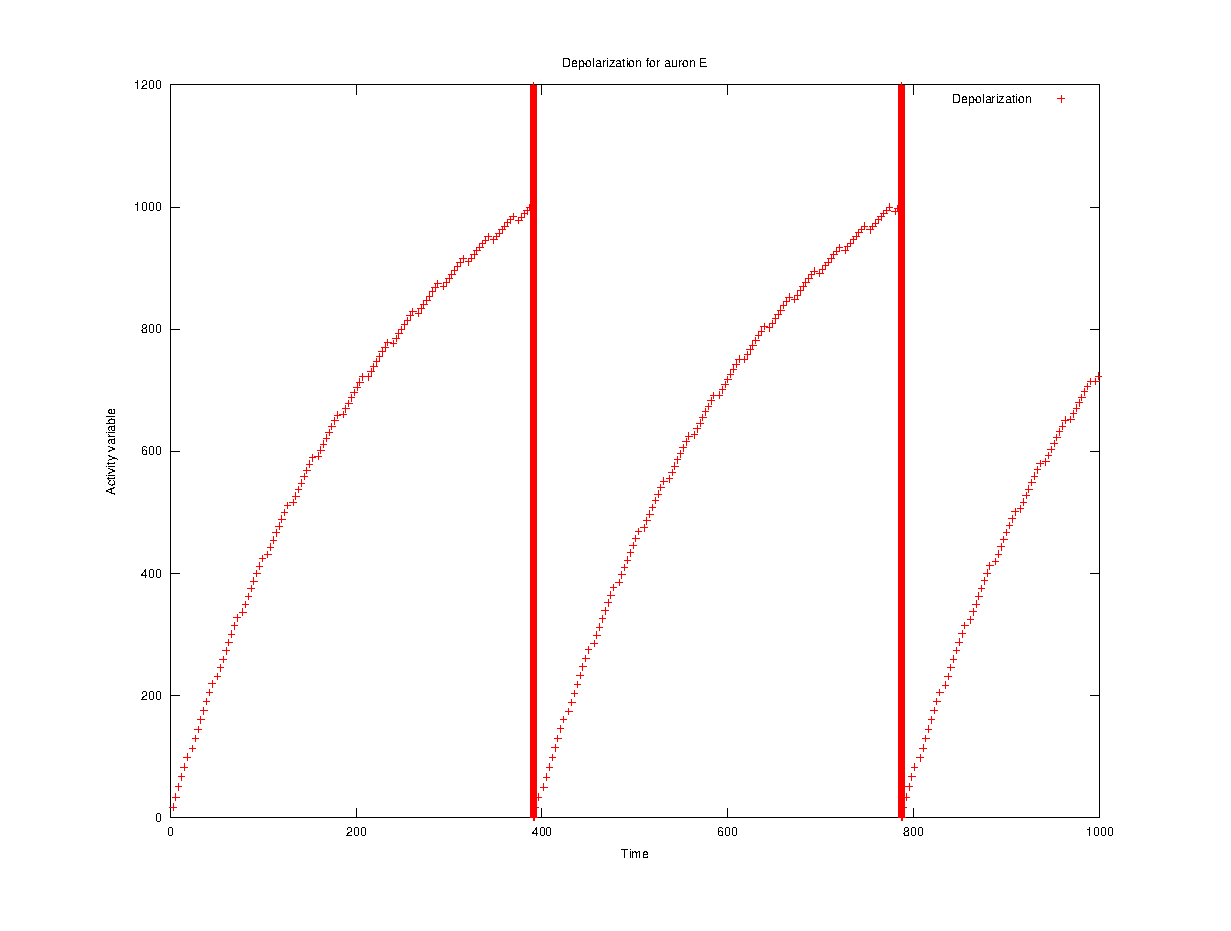
\includegraphics[width=0.95\textwidth]{depolPlotAvSN/eps_auronE-depol.eps}
		\caption{Depolarization plot for auronE in the neural circuit from fig ?. The activity variable for a SN corresponds to the depolarization of a neuron.} %TODO TODO Lag plot som beskriver kretsen, og referer dit, her.
		\label{figAuronE}
	\end{figure}

	Each time iteration, the value of the node will diminish due to ``leakage''. 
	In this implementation, the leakage is only computed whenever the value is used.
	This is done by the use of equation \eqref{eqLeakageForSANN}.

	%Skriv først (underveis i neste avsnitt) at for å teste dette kan vi lage en "neural oscillator", en krets som vil holdes aktiv av seg selv. Kvar output .. osv...
	To test the implementation of the SN, the circuit in fig. ? % XXX TODO Lag denne, og :  \ref{}
		was tested. The connections between node A1 and node A2 has a synaptic weight of weight $W_{21}=1$, large enough to excite node A2 above firing threshold in a single transmission.
	Each of the nodes A1-A9 has a synapse to the next node with a synaptic weight of one. 
	From node A9, there is a synapse to node A1 of weitht 1 completing the ``neural oscillator''. In this circuit each of the nodes will fire once every ninth time iteration.

	Except from node A7, every node in the ``neural oscillator'' have a synaptic connection to node E with a constant synaptic weight $W_{Ej}=0.017$ . %todo: ta vekk "constant" ?
	There is no synapse from A7 to node E.
	%From each of the nodes in the ``neural oscillator'' except for node A7, there is a synaptic connection to node E with a constant synaptic weight $W_{Ej}=0.0017$ .
	In the course of one period we therefore get eight excitatory inputs to node E, each transmission of size $W_{Ej}*\tau = 17$. Every ninth time iteration we get no input to node E.
						%period AV KA? Skriv kva!

	Fig. \ref{figAuronE} shows the resulting depolarization plot of node E. 
	We can se that node E gets a steady input from the nodes of the ``neural oscillator''.
	%
	Every cycle of the oscillator there is a pause in the excitatory input to node E, resulting in a small drop in node E's activity variable. 
	One cycle of the oscillator is represented by 8 entries in the log file, one log entry after each transmission.
	This can also be observed in fig. \ref{figAuronE} by remebering that during a pause in transmission, the change of value for the node is only due to the ``leakage'' of the node's value.
	Every 8'th value of node E's value is smaller than the previous entry due to this effect.
	%This is due to the absense of excitatory input and due to the leakage during the pause in excitatory input to the node.

	%After the pause in synaptic input to node E, the leakage is calculated at the time of the next transmission by eq. \eqref{eqLeakageForSANN}, resulting in the little drop in the node's value.

	% TODO flytt neste linja litt ned (eller noke, passer ikkje akkurat her..)
	Fig.\ref{figAuronE} is a direct result of the execution of the log files created by the simulator.
	% TODO Skriv det under i "log-file"-biden av design.tex! Passer ikkje her...
	%The constructor of every node creates a log file and each time the nodes activity variable is changed, the time iteration and the new value is written to the log file.
	%The destruction of each node finalize the node's log file, by writing octave calls that makes plots like the one in fig. \ref{figAuronE} and prints the resulting plot to an eps file.
	%Many of the eps files included in this report comes from the execution of similar octave script--file logs.

	We can also se that the mechanisms behind firing an action potential works. 
	%When the value of the node goes over the firing threshold an action potential is fired.  %XXX Dette er kanskje bedre måte å sei det enn neste?
	When the node's value goes to suprathreshold levels, an action potential is fired. %Skriv: dette er representert ved en vertikal strek i figuren (eller i logg-plottet).
	In fig. \ref{figAuronE} we can se that the node's value is reset to zero after firing an action potential.
	%TODO Ta med det neste, men ikkje før eg er heilt sikker, og kan gjøre det til meir enn en påstand (ta med noke i appendix, eller skrive tidspunkt for de to)
	%In the corresponding log file for the synaptic transmission of node E's output synapses, it can be observed that the synaptic transmission comes two time iterations after the node's value reaches the firing threshold. 
	%%Similar plots of the synaptic transmission from the synapses log file shows transmission after the time delay caused by the initiation of an action potential and the delay caused by the action potential propagating through the axon.
	%TODO Være sikker på at det er har skrevet her er heilt rett. (flaut dersom det er en åpenbar feil, her!)
	Analysis of the log files shows that node E fires one action potential at time 391 and one at time 787.
	The synapse's log file shows transmission at time 393 and 789, each at two time steps after node E's value goes above firing threshold.
	%each transmission at two time iterations after node E's value goes above the firing threshold. 
	This tells us that the simulated delay caused by the action potential initiation and propagation works as designed.
	% Auron E: AP    på tid: 391 og 787
	% Syn overføring på tid: 393 og 789
	
	The log entry for the next time iteration is zero, due to the simulated refraction period of the node.
	Two time iterations after the action potential the node's value becomes or 17. %TODO? Skal eg skrive litt om at eg kjører størrelse på W_ij i kor mykje postsyn. går mot fyring. I promille? Viktig poeng!
	%Har sjekka: Dette gjelder for begge overføringene/AP i simuleringen. Skriv dette, og at det betyr at vi for desse to overføingene faller "pause" ikkje til to tidssteg etter fyring.
	This corresponds to the defined synaptic transmission for each of the synpses of the circuit. %Kanskje heller : ".. for the synapse in question"? ELLER at dette betyr at i desse tilfellene har vi ikkje pause på dette tidspunktet.

	%This analysis shows that the above discussed design of the simulated neuron gives us the mechanisms of the neuron, in respect to synaptic transmission, leakage, refraction time and action potential firing.
	This analysis shows that, in respect to synaptic transmission, synaptic leaky integration, refraction time and action potential firing, the design and implementation gives the behaviour of the model used. 
																																														  %ELLER: .. considered model of the neuron.
	%TODO Skriv om den siste linja litt. (siste bit: kanskje heller: "... , the design and implementation gives the desired behaviour for the simulated neuron."?




%	\subsection{Analysis of the SN's value curve}
	% TODO TODO TODO TODO TODO TODO TODO TODO TODO TODO TODO TODO TODO TODO TODO TODO TODO TODO TODO TODO TODO TODO TODO TODO TODO TODO TODO TODO TODO TODO TODO TODO TODO TODO 
	% Gjennomfør ei analyse av kurva. (Meir enn/istedenfor den siste linja over).
	% TODO TODO TODO TODO TODO TODO
	%We can se that the value of the node has a vaulue % at det varierer som plot X (finn eit plott, legg det inn i BiologiskeSystemet.tex, referer dit, her) %TODO
%	Fig. \ref{figAuronE} resemples a plot of a step responce of a condencator, with an extra non--linearity when the value of the node crosses the firing threshold.
%	We have already analyzed the 
%	Skriv at kurva ser rett ut.





	



% Feil ved denne forenklinga:
%  - vi går ut fra at verdien ikkje lekker mellom dendrite og axon hillock. Dette er nok litt feil, men ikkje mykje.
% 	Dersom vi hadde hatt dette, måtte vi implementert lekkasjen, men også en liten time delay før verdien blir lagt til verdien i axon hillock. Dette er computationally ineffektivt.
% 	Dersom dette skal implementeres (at programmet skal være en simulering av neurale system, så er dette mulig ved å ha en egen node for axon hillock)
	
	
	%TODO Skriv korleis dette kan gjøres for KN.

	% Lag diagram om korleis dette funker. Kanskje eit "uml-signal diagram"?   (Treng fleire figurer her!)

	% TODO Lag en figur som viser oppsettet til kretsen.



%TODO TODO Lag eit plott som sammenligner kontinuerlig lekkasje, vs beregning av lekkasje etter 30 iterastions. (Dette skal inn her..)






% (Neste som kommer er KANN--implemenasjon-kapittelet)


% Implementasjon for KANN. Korleis gjør eg det? Kva er viktig?
% Mangler?

%TODO Skriv litt om: halv dag.
%
% PLAN:
% - ta med "propagating of kappa". At metoden brukt er antagelig ikkje den mest effektive, men det gjøres likt for å lage det meir egna for sammenligning.(ligger i implementation.tex)
% - ta med "om oppsamling av kappa" (ligger i implementation.tex)

% Kan sei at dette er "original work by the author." Dette kan ivertfall brukes når dette kapittel blir referert til!

%TODO Skriv om mealy automata, ANN, input som aktivitetsvariabel for 1.gen. og 2.gen. ANN og state som aktivitetsvariabel for 3.gen. ANN.
% 	Kan da skrive at denne modellen har aktivitetsvariabel for både state og input (Kappa, dDepolAtStartOfTimeWindow), og kan dermed lett transformerer KANN's aktivitetsvariabel over til 1g.ANN, 2g.ANN og 3g.ANN!
% 	Sjå [ ref_asdf2143@ANN ] i ANN.tex.

%*********************** KANN ***************************
\section{KANN design and implementation}
\label{secKANN}
	
	We have seen that the SANN model calculates the firing time of each node as a reactive event, after the value of the node goes above threshold.
	By the use of the equation presented in sec. \ref{secMatematiskModelleringAvBioNeuron}, an ANN could be designed to follow the same scheme.

	If the constantly updated estimated firing time is used, the scheme for the calculation of firing for the node will be different.
	%It could also use the constantly updated estimatet firing time.
	When the estimatet firing time is the same as the current time iteration, the element's task is executed.
	The task is therefore scheduled for execution at the estimated firing time.
	This gives a proactive model for determining the firing time.

	Another aspect is that the value of the node only has to be calculates when accessed.
	This gives that the ANN possibly is more effective than ANN based on direct simulation of the neuron.
	The equations presented in sec. \ref{secMatematiskModelleringAvBioNeuron} also gives a time--invariant activity variable.
	In addition to being more effective, this does not involve global trunction errors from the integration of time effects for the activity variable.
	As the value of the node is calculated when needed, both the error from trunction errors and the computational load introduced by the calculations will be decreased.

	In this section, different an ANN model is designed by the use of equations from sec. \ref{secMatematiskModelleringAvBioNeuron}.
	Only the aspects that differ from the SANN model will be presented. 
	
	%Skriv også det som står i T ODO over, eller i ANN.tex: [ ref\_asdf2143@ANN ]% Søk etter ref_asdf2143@ANN i fila ANN.tex.
	%As we will see, this new model uses both the state of the node at the start of the presente time window and the synaptic input to the node, $\kappa_{ij}$ to calculate the output of the node.

	%As we will see, this new model for ANN have both a state and output given by the last time iteration's state and the input to the node. 
	%This gives that the node is able to communicate with all the previous forms of ANN, and might serve as an important transform between different models of ANN."



 		\subsection{The Activity Variable} %TODO I Implementasjon:SANN er det viktig at eg skriver at aktivitetsvariabelen er brukt til depol til noden. (da blir teksten under rett)
	% This value is given by the input and the grade of leakiness.
	% Ta vekk den over(kommentert ut), eller siste bit av den under.

	As seen in section \ref{secMatematiskModelleringAvBioNeuron}, $\kappa$ is given by the input and the grade of leakiness of the node.
	For changing $\kappa$, we introduced the concept of a \emph{time window}. 
	A time window is defined as a period of time where $\kappa$ is constant within the current interspike period (see section \ref{ssecVariableInputBetweenSpikes}).
	By using eq. \eqref{eqVerdiligninga} it is possible to find the depolarization value of the node at any time $t \, \epsilon \, p_{isi}$.
	We can therefore use $\kappa$ as the node's activity variable, even if we use a reactive model for calculating spike time(like in the SANN model). 

	%TODO TODO Skriv på nytt! Skriv også at det er mulig å kalkulere f=p^{-1}. Desse tre elementa gjør det mulig å kommunisere med alle de tre tiligere generasjonene ANN (men ikkje skriv "tidligere")
	If $\kappa$ is used as the activity variable, more than the depolarization value of the node can be calculated by its activity variable. 
	In section \ref{secMatematiskModelleringAvBioNeuron} we have seen that both the firing time and the period corresponding to the activity variable can be calculated when we use $\kappa$ as the activity variable.
	%By using that the frequency is the inverse of the period,  it ...
	% % XXX TODO TODO Passer bedre i konslusjon!
	As it is possible to calculate the corresponding frequency for any given activity level $\kappa$, it is possible for a $\kappa$N to communicate with a node of the second generation ANN;
	%It is therefore possible to use a node based on the mathematics present in section \ref{secMatematiskModelleringAvBioNeuron} as an interface to each of the other generations ANN.
		To interface with a second generation ANN, we can use that the frequency is the inverse of the period. 
	The period is calculated from eq. \eqref{eqHeilePerioden}.
	%The $\kappa$N can as easily get input from as sending output to a node of a second generation ANN. 


\begin{figure}[hbt!p] 
	\centering
	%
   	\subfloat[Value function for $\kappa=10.1 \,\text{, } \tau=10$]{\label{figDemonstrasjonAvFrekvAvKappa:edge-a} 						\includegraphics[width=0.5\textwidth]{pdfVerdifunksjonen_med_terskel_T_10__K_10komma1.pdf} 		}  
   	\subfloat[Value function for $\kappa=12 \,\text{, } \tau=10$]{\label{figDemonstrasjonAvFrekvAvKappa:edge-b} 						\includegraphics[width=0.5\textwidth]{pdfVerdifunksjonen_med_terskel_T_10__K_12.pdf} 		}  
	%\caption{Demonstration of the value function for changing kappa}
	\caption{ 	( \ref{figDemonstrasjonAvFrekvAvKappa:edge-a} ) The value fuction with $\kappa=1.01\cdot\tau$ and   
				( \ref{figDemonstrasjonAvFrekvAvKappa:edge-b} ) The value fuction with $\kappa=1.2\cdot\tau$
			} %TODO skriv om dette tomrommet i teksten under.
	\label{figEdgeTransmission}
\end{figure}




	% TA VEKK? Blir så veldig svevende.. Fin tekst, men får følelsen av at dette er fiction.
	%The first generation ANN were stateless, and the ouput only varied with the immediate input. 
	%This demands a different kind of transduction mechanism, but because the first generation ANN could be said to be obsolete, no more time will be used on this.
	%The most important 
	%
	%In a $\kappa$N, the activity variable can therefore represent $\kappa$ instead of the depolarization of a corrsponding neuron.
	
	If a suitable scheduler is devised, $\kappa$ could be used effectively for planning, or ``estimating'' the firing time of the node.
	The rationale behind the use of the word estimate is that the estimated firing time will change every time the activity variable changes, possibly before the initially calculated firing time. 
	The firing time is then updated. 
	The first firing times computed by eq. \eqref{eqRemainderOfPeriod} is therefore but a naive estimate of the firing time of the node.
	As the time of firing of the node approaches, the estimated firing time becomes more certain.
	When the present time iteration is the same as the estimated firing time, the estimated firing time is exact; The node's value is now above firing threshold.
	
	%The estimated firing time is computed by eq. \eqref{eqRemainderOfPeriod}, and will be firing time of the node given that the present time window last until firing (no change in $\kappa$ for the remainder of the period).

	%Because of time limitations for this project, effectivity analysis have not been conducted. %Litt rart språk! XXX conduct conduct!

	
	%\subsection{Updating $\kappa$} %Calculation and recalculation of $\kappa$
	\subsection{Synaptic transmission}
	\label{ssecSynTransForANNliggeriKANNsection}
		%TODO Skriv om, med kontinuerlig tanke på kappaANN. F.eks. : in biology, AND IN SANN, a synaptic ...

		% skrive om korleis synaptic transmission fåregår (generellt (om at $\kappa_{ij} = \frac{W_{ij}}{p_{pre}}$ ).
		In biology and in the SANN model, a synaptic transmission change the value of the postsynaptic node.
		Because we do not use the depolarization value as the activity variable in a $\kappa$N, this form of synaptic transmission makes the model a bleak copy of SANN.   %XXX eller bare " a compy of SANN." Nee. Men bleak er dårlig.
																							% , this form of synaptic transmission will not work. %TODO TODO SKriv om! XXX
		A better approach is to develop a separate model for synaptic transmisson in $\kappa$ANN.

		For second generation ANNs, synaptic transmission is defined as the synaptic weight times the number of incoming spikes per time step.
		This can be formalized as
		\begin{equation}
			u_{ij}(t) \, = f_{j} \cdot w_{ij} \cdot \Delta t
			\label{eqSynapticTransmissionFor2genANN}
		\end{equation}
		Where $u_{ij}(t)$ is the control signal from node $j$ to node $i$, $w_{ij}$ is the size of the synaptic weight %between node $j$ and node $i$ 
			and $f_j$ is the presynaptic node's firing frequency.
		Because $\kappa$ANN contains elements from both the second and third generation ANN, it is not given that we can use either of these transmisson rules.

		%Eq. \eqref{eqSynapticTransmissionFor2genANN} states that the contribution from node $j$ to node $i$'s activity variable is a function of the frequency of the presynaptic neuron.
		Inspired by \eqref{eqSynapticTransmissionFor2genANN}, we define synaptic transmisson in $\kappa$ANN as the synaptic weight times the activity variable's corresponding frequency.
		By combining eq. \eqref{eqHeilePerioden} and \eqref{eqSynapticTransmissionFor2genANN} and using that $f_j = \frac{1}{p(\kappa_j)}$ we get
		\begin{equation}
			\kappa_{ij}(\Delta t) = \frac{ w_{ij} }{ p_{isi}(\kappa_j)} \cdot \Delta t  %XXX  Verifiser at alt passer inn, no (at var.navn er rett osv)
		\end{equation}
 		
		$\kappa_{ij}$ here defines the synaptic transmission in the connection between node $j$ and node $i$.
		% XXX Bare ta med når du finner ut HEILT kva som er effekta av det motastte XXX :  If the time step large enough, we can define that each synaptic transmission lasts for one time step.
		For simulations with constant time steps, $\Delta t$ is constant and can be incoorporated into the synaptic weight $w_{ij}$.
		We get the equation used for synaptic transmission in $\kappa$ANN.
		%If we define the transmission of the synapse between node $j$ and node $i$ as $\kappa_{ij}$ we get the equation for synaptic transmission:
		\begin{equation}
			\kappa_{ij} = \frac{ w_{ij} }{ p(\kappa_j)}
			\label{eqSynapticTransmissionForKANN}
		\end{equation}

		This equation is a simplification of the biological synapse, as it does not take into account the timing of successive transmissons and other time elements of transmisson 
																							%short--term synaptic plasticity as a consequence of rapid transmissions (see appendix \ref{appendixSecPresynapticSynapticPartOfTransmission}).
			(see appendix \ref{appendixSecPresynapticSynapticPartOfTransmission} for an introduction to synaptic potentiation). 
																					%a discussion of time elements in transmission in the biological synapse ).%eller heile appendix A (syn. trans.)

		%TODO TODO TODO TODO ENTEN : skriv først at for ei synapse-neuron så er K_i lik K_ij
		%TODO TODO TODO TODO ELLER : Skriv direkte at K_i er summen av input (bruk ord som lineær karrakteristikk, superposisjon, osv.)
		The typical neuron has numerous input synapses. 
		%How does \eqref{eqSynapticTransmissionForKANN} expand to multiple synapses?
		%
		%TODO Skriv om: No er det for sein, og eg tenker ikkje beint.
		As for temporally separated input, the synapses' total effect of multiple transmissions is modelled as a linear carracteristic. %TODO TODO Skriv kvifor / begrunn dette valget!
		%This gives that the postsynaptic potential is the sum over all the input nodes' transmission.
		% %Just as the input of many ``simultaneous'' transmissions has a linear carracteristic, the input through multiple synapses be 
		%
		%This model of synaptic transmission does not take into account 
		For nodes with multiple input edges, the activity variable $\kappa_i$ is the sum of the contribution from each of its input synapses.
		%jeje Skriv om det på slutten, setninga over. Kanskje  					 is the sum of all the contributions from different input synapses. (?) XXX XXX
		\begin{equation}
			\kappa_i = \sum_j{\kappa_{ij}}
			\label{eqSumOfKij}
		\end{equation}

		The effect of each synaptic transmission can therefore be decoupled from the other synaptic transmissions when calculating the postsynaptic effect of a transmisson.
																				%the rest in the calculation of the postsynaptic node's activity variable, $\kappa_i$.



		%In discrete--time systems, we can define every synaptic transmission to last for one time iteration (if the time step is large enough).  % MED ELLER IKKJE: "(if the time step is large enough)" ??? XXX
		%This causes $\Delta t$ to become constant. We can incoorporate this constant into $W_{ij}$.

%		For an ANN based on the activity variable $\kappa$, as previously introduced in chapter \ref{secMatematiskModelleringAvBioNeuron} %TODO Sjekk denne  referansen bedre / skriv bedre (?).
%		eq. \eqref{eq SynapticTransmission} is highly relevant.  % highly relevant skurrer litt. Det er veldig relevant. Finn synonym..
%		If we define $\Delta t$ to be some constant, and incoorporate this constant into $W_{ij}$, we get the equation for the synaptic transmission of the activity variable.
%		We call the size of this transmission for $\kappa_{ij}$.


		%For nodes with multiple input synapses, the activity variable $\kappa$ is the sum of all the contributions from different synapses. %VERIFISER DETTE! Vær heilt heilt sikker på at K=sum(K_ij)
		%We can write this mathematically as 
		%\begin{equation}
		%	\label{eqSumOfKij}
		%	\kappa_i = \sum_j{\kappa_{ij}}
		%\end{equation}
		%
		%In this way the synaptic transmission of the individual synapses can be decoupled from the postsynaptic activity variable, $\kappa_i$.
		

		\subsection{The Postsynaptic Effect of Synaptic Transmissons}
			\label{ssecSynInputToANodeKANN}
			Equation \eqref{eqSumOfKij} defines the postsynaptic effect of transmissions from multiple input synapses.
			In pragmatic ANNs the effectivity of the implementation is an issue, and an attempt has been made to make the calculation of the node's activity variable more effective.
			
			% As we will see, ... (det under) .  		No fremstår det som en ubegrunna påstand. XXX
			If we define a transmission in the edge as the derived of the corresponding synaptic transmission, we will see that this makes the implementation more effective.
			\begin{mydef}
				Let $\kappa_{ij}$ be the synaptic transmission. The edge transmission in $\kappa$ANN is given by $u_{ij}(\kappa_j) = \Delta \kappa_{ij}$.
			\end{mydef}
																												%updating the postsynaptic node's activity variable after a transmission becomes more effective.
			The synaptic transmission now becomes the integral of all the edge's transmissions, modelled by %eq. \eqref{eqSynapticTransmissionAsSumOfEdgeTransmissions}.      %, and is defined as
			\begin{equation}
				\kappa_{ij} = \sum_t{u_{ij}(\kappa_j)}
				%\kappa_{ij} = \int{u_{ij}(\kappa_j)} \, \mathrm{d}t
				\label{eqSynapticTransmissionAsSumOfEdgeTransmissions}
			\end{equation}
			
			Where $u_{ij}(\kappa_j)$ is the transmission through the edge.
			This involves that a new transmission updates $\kappa_{ij}$ by adding its value to the current $\kappa_{ij}$.
			%As the postsynaptic node's activity variable is the sum of all the synaptic transmissions, as defined in \eqref{eqSumOfKij}, transmission through 
			As the postsynaptic node's activity variable is the sum of all the synaptic transmissions, and each synaptic transmission is the integral of all the transmissions through the edge, 
				$\kappa_i$ can be updated by simply adding the new edge transmission to $\kappa_i$.
			%VIKTIG XXX Skriv litt om at Kappa er fullstendig time-invariant. Viktig for modellen, og ikkje heilt selvsagt!

			In the previous paragraph, we used two 		 different expressions for transmission through a connection between two nodes. 
			%We have in the previous paragraph used two
			The synaptic transmission $\kappa_{ij}$ is used as the amount $\kappa_j$ transmitted by the connection between node $j$ and node $i$. 
			The edge transmission $u_{ij}(\kappa_j)$ is used as the transmission from node $j$ to node $i$ in the implementation. 
			These two transmissions differ if the implementation's solution is different than a direct implementation of eq. \eqref{eqSynapticTransmissionAsSumOfEdgeTransmissions}.
			%A discussion 
			% FEIL: The choice for this implementation is presented in the next section (sec. \ref{ssecImpOfSynTransmissionKANNN}).
			For this implementation the edge transmission is previously defined as the change in synaptic transmission. 
			%The fact that these transmissions differ follows a solution for making the implementation more effetive.


			Each edge's transmission is completely decoupled from the others' transmissions.
			Each synapse's transmissions can therefore be calcutated separately.
			In an object mode, this is very good for encapsulation as each synapse can update its own $\kappa_{ij}$.
			%This is completely decoupled from the other transmissions, and each edge transmission can be calculated by the edge at the time of transmission. 
			%This is wery good for encapsulation in an object oriented programming language.

			After each time iteration, the postsynaptic node's activity variable is updated as the sum of all the synapses with an altered level of transmission.
																																%  changed         ?

			%For synapses transmitting the derived of $\kappa_{ij}$ we only have to integrate this change of transmission from all the input synapses with a changed level of transmission, and get
			\begin{equation}
				\kappa_i = \sum_c{\kappa_{ic}}
				\label{eqSynapticTransmissionForKANNimplementation}
			\end{equation}
			Where $\{c\}$ is a subset of $\{j\}$ consisting of all the presynaptic neurons where the activity variable has been updated.

			% KANSKJE: skrive at kappa er tidsinvariant, og varierer bare med kappa_ij. Dette gjør ting lettere.

			%In the implementation of $\kappa$ANN we call the nodes for K\_auron.
			%The synaptic input for the activity variable of a K\_auron is defined by \eqref{eqSumOfKij}.
			% %To avoid having to recalculate $\kappa_i$ from \eqref{eqSumOfKij} every time the transmission of a synapse changes, we can implement synaptic transmission as the transmission of the derived of $\kappa_{ij}$.
			%To avoid recalculation of $\kappa_i$ from all the input synapses when one synapse changes its transmission, this implementation defines edge transmission as the derived of $\kappa_{ij}$.
			%Now the postsynaptic $\kappa_i$ can be calculated without summing all the synapse inputs after changed input at one of its edges.
			% %In this case the postsynaptic $\kappa$ can be recalucated without summing all the synaptic inputs every time one synapse changes its transmission.

			To sum up the analysis in this seciton, edge transmission of the implementation is defines as  $u_{ij}(\kappa_j) = \Delta \kappa_{ij}$.
			For each edge transmission the synaptic transmission $\kappa_{ij}$ is the integral of all edge transmissions, and is updated by simply adding the new edge transmission.
			The postsynaptic node's activity variable $\kappa_i$ is the sum of all it's input transmissions, and is updated by the same principle; %var: , and can be updated ..
				After an edge transmission $u_{ij}(\kappa_j)$, $\kappa_i$ is updated by simply adding $u_{ij}(\kappa_j)$. 
			%The operation of taking the sum over all the node's input synapses after a change in one input transmission is thus avoided.
			%The operation of taking the sum over all the node's input synapses, after a change in transmission for a subset of the input synapses is thus avoided.
			 The operation of taking the sum over all the node's input synapses after a change in one $\kappa_{ij}$ is thus avoided.

			%We can, in other words, add the change in synaptic transmission, $\Delta K_{ij}$, to the postsynaptic activity variable to get the updated activity variable, $\kappa_i$.
			%The edge transmission in the implementation is defined as $u_{ij}(\kappa_j) = \Delta K_{ij}$, so for each edge transmission the postsynaptic node's activity variable is by simply adding $u_{ij}(\kappa_j)$.
			%This can be done at the time of each transmission, and without having to consider any of the other synaptic transmissions to the node.
			
			%XX Skal eg skrive dette her: XXX Dette står vel i neste avsnitt?
			%If we wait until after the current time iteration before calculating the effects of the changed kappa, much calculations will be saved.




			\subsection{Implementation of Synaptic Transmission}
			\label{ssecImpOfSynTransmissionKANNN}
	
	%		Begynn med å skrive at det er er vankelig å vite når det skal skje. Diskuter litt fram og tilbake som intro til section. %TODO 
	
			The synaptic transmission is given by $\kappa_{ij} = w_{ij} \, \cdot \, p_{isi}^{-1}(\kappa_j)$, the synaptic weight multiplied by the inverse of the inter--spike period.
			%In this implementation, $\kappa$ is used as the activity variable instead of the node's depolarization, and an other transmission scheme needs to be devised.
			Edge transmission is in this implementation defined as the change in synaptic transmission, or $u_{ij}(\kappa_j) = \Delta \kappa_{ij}$
			%This itroduces mechanisms that makes it redundant to perform the sum over all the node's input synapses every time one synapse's $\kappa_{ij}$ is updated.
			This introduces mechanisms that makes computational of the sum over alle the node's input synapses redundant, as more effective methods are used. %TODO skriv om!
			%TODO finn ut korleis eg skal skrive det over / which of dei to setningene eg skal basere setninga på..
	
			%%\subsubsection{Implementation of transmission through a synapse} % Vettafaen om denne skal være med. Gjorde om fra å være en kommentar, no..
			When implementing synaptic transmissions, equation \eqref{eqSynapticTransmissionForKANN} is considered first.
			This equation is based on the presynaptic inter--spike period and the synaptic weight of the edge, elements that are available from the presynaptic node and the synapse itself.
			At the time of transmission, the edge transmission is further calculated as the change in $\kappa_{ij}$.
			
			When $\kappa$ is changed, a new time window is commenced. 
			The node's initial depolarization in the new time window is calculated as the value of the node at the end of the previous time window.
			With the starting value for the node's depolarization, the further depolarization curve and the estimated firing time of the node can be calculated by eq. \eqref{eqVerdiligninga} and \eqref{eqRemainderOfPeriod}.

			A time step is defined as the smallest iteration in time.
			The first time the effect of a changed $\kappa$ may appear is thus after the current time iteration.
			As we potentially get multiple edge transmissions each time iteration, many calculations can be saved by calculating the effect of changed $\kappa$ after the current time iteration.
			For every edge transmission we only add the new transmission to the current $\kappa$.

			Every time a node's $\kappa$ is changed, a pointer to the node is inserted into a list \emph{pCalculateTaskQue}, introduced in section \ref{ssecCalcultaionTaskQue}.
			This list is a static element of \emph{time\_class}, and only one instance of the list is constructed. 
\begin{lstlisting}
static std::list<timeInterface*> pCalculateTaskQue;
\end{lstlisting}
			This list is specifically designed to keep an overwiev of \emph{timeInterface} derived classes in need of post--iteration calculations. %todo skriv om!
%			One example of this is a node after a changed $\kappa$. %in it's activity variable, $\kappa$.
			Before time is iterated by \emph{time\_classes::doTask()}, \emph{time\_class::doCalculation()} is called.

			The first task of \emph{time\_class::doCalculation()} is to make shure that every entry of \emph{pCalculateTaskQue} is unique, by removing every duplicate entries of each element of the list.
			After this, \emph{time\_class::doCalculation()} calls each entry's doCalculation() function.
			% TODO Neste to linjene hører heime i design.tex:
			The \emph{doCalculation()} function is defined as a pure virtual fucion in the \emph{timeInterface} class, assuring that every object of a derived class have defined it own \emph{doCalculation()} function.
			%meaning that every class inheriting this function have to implement the action of this function for the class.
			%If it does not, the derived class will inherit the interface aspect of \emph{timeInterface}, and cannot be made an instance of. %TODO Skriv om!
		
			In class \emph{K\_auron},  the \emph{doCalculation()} member function is responcible for updating variables dependent on $\kappa$.
			%The \emph{doCalculation()} member function of class \emph{K\_auron} calculates the effect of a changed $\kappa$.
			In this way equation \eqref{eqSynapticTransmissionForKANNimplementation} is implemented during each time step, and the calculation of the updated effect of the new $\kappa$ is executed at the end of the time step.
			The more strenuous task of calculating the initial values of the new time window and the effect of the changed $\kappa$ for the node is thus called at most once for every time iteration.

%\begin{lstlisting}
%static std::list<timeInterface*> pCalculateTaskQue;
%\end{lstlisting}


	
% Setninger som inneheld aspekt som eg ikkje har dekka:
		%	When $\kappa_i$ changes for a node, we need to recalculate the inverse of the period for this new $\kappa_i$ to get the synaptic transmissions right.
		% Synaptisk transmission er resultat av p^-1 Dette er ikkje skrevet over.

		% uvisst kva delay før propagation av kappa skal være.


	
	

%			As we allways calculate the next value as a funcion of the previous value and the new input, we will get an integration of the local truncation errors, and possibly get an error of some size.
%			This effect is often referred to as ``the global truncation error''.

% TODO Hugs å skrive om dette:
% 		The most imminent effect is the possibility of an integral error from integrating the derived to get the new $\kappa_i$. 
%		This is important, and a whole section is dedicated consideration of this (se sec. \ref{ssecRecalcKappa}).
% _____________________ fiksa til hit __________________________________________________________________________________________________________________________________________________________________________________


		\subsection{Relcalculating $\kappa$}
		\label{ssecRecalcKappa}
		Defining the edge transmissions as the derived has many positive sides when we consider efficiancy of the implementation. 
		%The negative sides comes when we consider the ease of implementation and the truncation error.
		The negative sides comes as a result of the truncation error.




		Because synaptic transmission is designed as the derived of the $\kappa_{ij}$ and the postsynaptic activity variable $\kappa_i$ as the integral of this kind of synaptic transmission
			, we have to consider the trunction error of $\kappa_i$. 
		Every small error in the calculated $\kappa_i$ will subsequently be a part of the result.
		We get possibility of large errors after a relatively short time.
		We should therefore recalculate $\kappa_i$ periodically.


		%For this reason it is important to recalculate $\kappa_i$ periodically.
		%One solution to this is to recalculate $\kappa_i$ periodically.
		For the recalculation of $\kappa$, a period with the right balance between recalculating to often and not often enough has been devised. %XXX Endre desse to setningene, dersom eg har tid. (siste eg gjør)
		If the recalculation happens to often, to much effort will go into recalculating $\kappa$, and if the recaluclation happens to seldom, a global trunction error of unacceptable size might emerge.

		The truncation error might vary with variables such as hardware architecture, system load and even the individual auron's activity level,
		Because it is hard to know the level of the individual auron's truncation error, the period between recalulation of truncation error is designed to be adaptive as a function of the last error.
	%	The time of the next recalculation of the auron's $\kappa$ is computed after $\kappa$ is recalculated, as a function of the error given from the present recalculation.

		%To best achieve this, the period between recalculating $\kappa$ is designed to be dynamic as a function of the error at the last recalcualation. 
		It is important to limit both the minimum and the maximum period between recalulations of $\kappa$.
		To achieve this, an altered sigmoid function has been devised for this purpose.
		This function gives a maximum value when the error is zero ($\lim_{E \to 0} p_e(E) \neq \infty$) and a positive minimal \linebreak
			period($\lim_{E\to\infty} p_e(E) \neq 0$).
		%This function should therefore have a maximum when the error is very small, and a minimum period as the error grows very large. 

		\begin{equation}
			\label{eqAlteredSigmoidFunk}
			p_e(E) = (c_1+c_2) - \frac{c_2}{1+e^{-(c_4*E-c_3)}}
		\end{equation}


		\begin{figure}[bht!]
			\begin{center}
				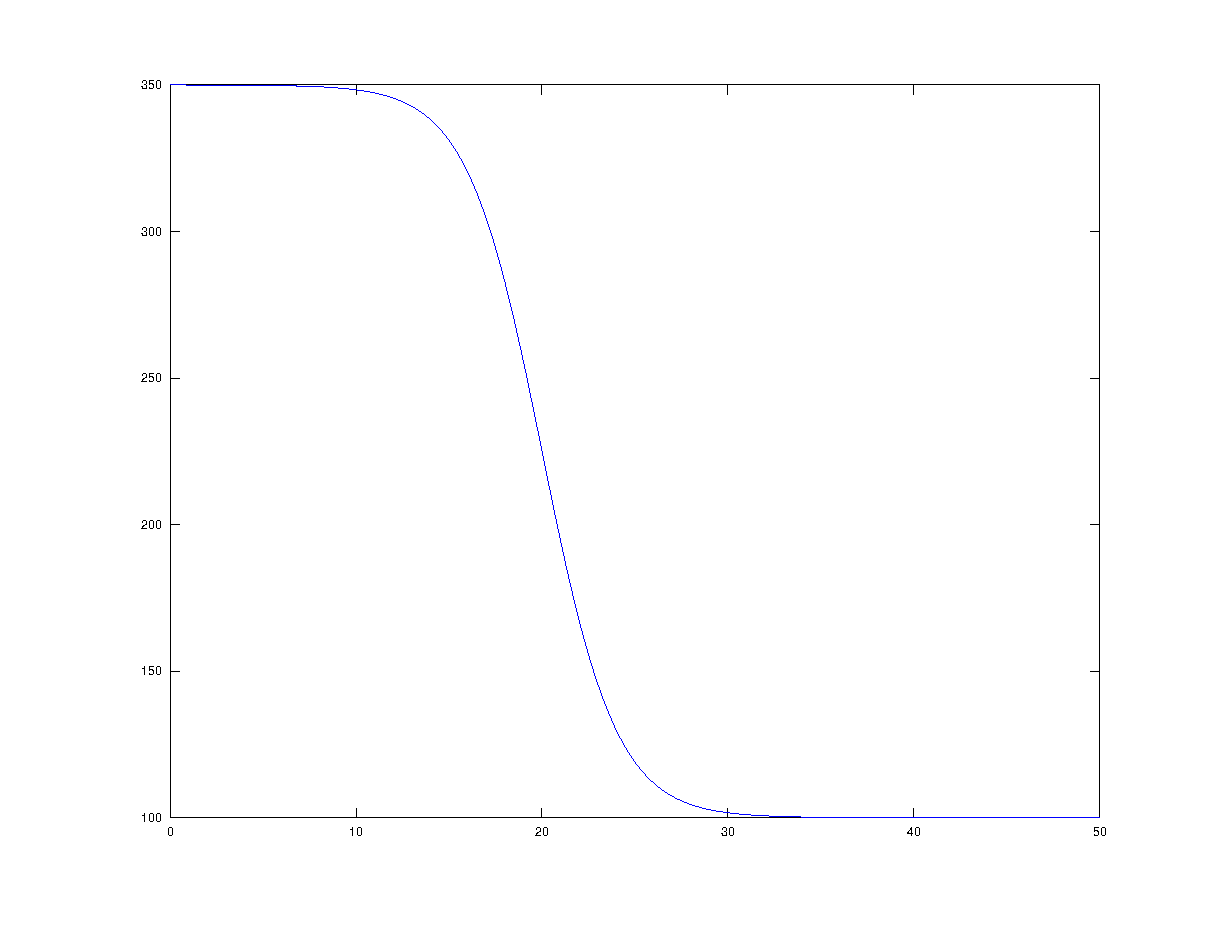
\includegraphics[width=0.95\textwidth]{sigmaPlot}
				%\caption{Demonstration of the value function for changing kappa}
			\end{center}
			\caption{Plot of the altered sigmoid function (eq. \ref{eqAlteredSigmoidFunk}), with \mbox{$c_1$ = 100}, \mbox{$c_2$ = 250}, \mbox{$c_3$ = 10} and \mbox{$c_4$ = 0.5}. 
					The minimum is given by the constant $c_1$.  }
			\label{figAlteredSigmoidFunction}
		\end{figure}
	
		This will give a the largest output value when the error is very small. For increasing errors, the output of the altered sigmoid function will become smaller.
		We can see from plot \ref{figAlteredSigmoidFunction} that the altered sigmoid function \eqref{eqAlteredSigmoidFunk} give a maximal and a minimal period for the recalculation of $\kappa$.
	
		From \eqref{eqAlteredSigmoidFunk} we can see that the altered sigmoid function has the maximum value of $c_1+c_2$.
		In fig. \ref{figAlteredSigmoidFunction} the values $c_1 = 100$ and  $c_2 = 250$, giving the maximum value as 350 time iterations between recalculation of $\kappa$.
		Because of a small degree of truncation error in the test cases used while testing this implementation, the minimal period between recalculation was set to $c_1=100$ time iterations. 
		This can easily be altered for situations where the truncation errors become an issue.
		% T ODO Skriv om det under. Blir overflødig..
		%The altered sigmoid function \eqref{eqAlteredSigmoidFunk} is used when the period to the next recalculation of $\kappa$ is planned. 
		%The maximum value, in this context, gives the maximum period before the new recalculation is done. %This happens when the error is wery small (se fig \ref{figAlteredSigmoidFunction}).
		%The minimal and maximal period between recaluclation can be modified by altering the constants $c_1$ and $c_2$.

		%TO DO skriv litt om, de neste to avsnitta.
		% T ODO SKRIV DETTE, MEN SKRIV OM FØRST :  One other thing that is worth noting is the variables $c_3$ and $c_4$ giving the shape of the curve. $c_4$ gives the lenght of the curve, that is how steep it is.
		



%		After some analysis, I decided to use the values used in fig. \ref{figAlteredSigmoidFunction}.
%		This gives a function that gives maximum period between recalculation of $\kappa$ when the error is below about 10. 
%		It has a relatively steep decent between an error of 10 and 30. The minimum period is set to 100 time steps and the maximum to 350 time iterations.
%
%		The minimum time between recalculation of $\kappa$ will limit the use of resources. %cause the simulation not to use to much resouces.
%		The maximum value of this function is limited because the error will have a stocastic nature, and one could e.g. end up with zero error if one get equal positive and negative errors.
%		This could potentially give a very large period before the next recalculation of $\kappa$.
%
%		Because of the stocastic element of the trunction error, the planning of the next recalculation of $\kappa$ is also implemented as a FIR--filter with a moving average over the last three values.
%		%For this reason, the calculation of the period between recalculation of $\kappa$ is also implemented as a FIR--filter with a moving average over the last three values.
%		%
%		%When the auron is constructed, $\kappa$ is recalculated before any input synapses is defined. This gives the filter a small initial period.
%		When the simulation starts, $\kappa$ is first calculated by the recaluclate function, giving the recalculate function a small initial period based on the level of synaptic input.
 		The first time $\kappa$ is calculated, it is calculated with the recalculate function, giving the filter a small initial period. %, based on the initial level of input.
		Aurons with a large initial input will therefore get a smaller initial recalculation period that some auron with a smaller initial input. %due to a large initial error.

		\subsection{Implementation of recalculation of $\kappa$}
		The execution of the planned recalculation of $\kappa$ is done in the same way as the execution of the planned action potential for the $\kappa$ auron.
		
		For recalculation of $\kappa$ with the chosen method, we need a separate object whose \emph{doTask()} function will call the \emph{K\_auron}'s \emph{recalculateKappa()} function.
		To achieve this, each \emph{K\_auron} has its own object of the class \emph{recalcKappaClass}.

		The function \emph{recalcKappaClass::doTask()} will call the associated \emph{K\_auron}'s \emph{recalculateKappa()} function.
		After $\kappa$ is recalculated, the next recalculation will be scheduled based on the error from this recalculation. 
	%	in addition to planning the time of the next recalculation according to the considerations in section \ref{ssecRecalcKappa}.
		

% HER EHER HER er eg.

		%Siden kappa bare regnes ut som integralet av den deriverte, vil det være behov for rekalkulering av Kappa, i ny og ne. Dette bør ikkje skje for ofte, heller ikkje for sjeldent.
		%Difor: lage en adaptiv utførelse av dette. Dette sjekker avviket mellom den rekalkulerte verdien og den gjeldende verdien, ved rekalkulering. 
		%
		%Dette avviket sjekkes opp i mot en predefinert ønska verdi, og differansen er med på å bestemme om periode til neste rekalkulering skal auke eller minke (auker/minker som en funksjon av avvik-avviket). 
		%
		%Dette avviket er m.a.o. med på å bestemme tid til neste rekalkulering av Kappa.
		%Auken/minken bør ha en maksverdi.



% % KAN ikkje denne takast vekk? XXX XXX XXX
% 	\subsection{Estimation of firing time}
% 	% Skriv kvifor eg kaller det "Estimation" og ikkje calculation.
% 	%TODO dette var en del av section{KANN} tidligere. Fokuset i teksten er det. Skriv om slik at det gjelder generelt, men med spesiellt fokus på KANN.
% 	%For KANN, edge transmission can be wieved as transmission of the change in the presynaptic node's input level.
% 	For $\kappa$ANN, synaptic transmission $\kappa_{ij}$ is given by eq. \eqref{eqSynapticTransmissionAsSumOfEdgeTransmissions}.
% 	Edge transmission is further defined ad the change in $\kappa_{ij}$, and gives the input of the postsynaptic node.
% 	%The input of a node, in terms of $\kappa$, is propotional to the synaptic weight and inversly propotional with the presynaptic inter--spike period.
% 
% %	When the presynaptic node changes its activation level, and its period increases or decreases, the level of synaptic transmission will be altered accordingly. 
% %	Because of the number of synapses per axon/ dendrite, it is most efficient to perform as many of the calucations as possible in the presynaptic auron.
% %	For this reason, the most efficient way of calucating the postsynaptic dendrite's activation level is to let the synapse transmit the derived of the signal (change).
% %	% Har skrevet dette tidligare. (to subsections før). Skriv om, og referer/underbygg denne måten.
% 
% 	
% %	If every $\kappa_{ij}$ but one, $\kappa_{ix}$, is kept constant, it can be shown that $\Delta \kappa_i$ is equal to $\Delta \kappa_{ix}$.
% % 	%Following this, $\kappa$ is calculated as a superposition of all the input synapses' contribution, these equations can be extended to change of transmission of multiple synapses.
% %	%This gives us the equation for the change of postsynaptic activation level following synaptic transmission at synapse from node $x$ to node $i$.
% %	We get that
% %
% %	\begin{equation}
% %		\kappa_{ij, new} = \kappa_{ij, old} + \Delta \kappa_{ij}
% %	\end{equation}
% 
% %	Instead of calculating all of this at every synapse, or for every synapse at the postsynaptic dendrite, it is better to calculate as much as possible presynapticlly.
% %	This gives one calulation every time a node fires an action potential, instead of one for every output synapse.
% 
% 	%X XX X XX  XX X Trur eg skrive  resten i subsubsection: implementation:KANN -> pEstimatedTaskTime -> execution of elements
% 	
% 	% TOD O SKRIV litt om dette her, og lag eit frampeik til etter pEstimatedTaskTime, der eg skal skrive meir om dette.
% 	%Transmission of the derived solves many problems concerning efficiency, but it also introduces integral error for the postsynaptic $\kappa_i$
% 	%This problem can be solved, and we will come out JAJAJ. Skriv anna gang-- TODO
% 
% 
% 	%Etterkvart: skriv om integral-errors og fiksing av dette ved å bruke pEstimatedTaskTime (regelmessig fiksing, som er adaptiv med basis i feilen på postsyn signal (høg feil=>oftere regelmessighet på resumming av kappa)).
% 
% 
% 	When the firing time is estimated, it is fundamental that we have a mechanism for executing these elements at the right time. 
% 	In the section \ref{secPlannedEvents} two different solutions has been proposed for this. 
% 	The section is concluded by presenting a discussion behind the choice for this implementation.
% 	%XXX BLÆ! skriv om linja over!
% 	%In section \ref{ssChoiceOfTimeEstimationForThisImplementation} the choice for this implementation will be presented, and different pros and cons with each method will be discussed.



%	\subsection{When do $\kappa$ propagate?} %TODO TODO Dette er analyse => Discursion! XXX XXX XXX XXX XXX XXX XXX XXX XXX XXX XXX XXX XXX XXX XXX XXX XXX XXX XXX XXX XXX XXX XXX XXX XXX XXX XXX XXX XXX XXX XXX XXX XXX 
%	In the start of this project, $\kappa$ANN were implemented as a varian of a network with spiking nodes.
%	Here the information is transmitted by the synapses following an action potential. 
%	Because the SANN model was the basis of this implementation, the information were originally transmitted at the time of the node spiking.
% %XXX XXX XXX XXX XXX XXX XXX XXX XXX XXX XXX XXX XXX XXX XXX XXX XXX XXX XXX XXX XXX XXX XXX XXX XXX XXX XXX XXX XXX XXX XXX XXX XXX XXX XXX XXX XXX XXX XXX XXX XXX XXX XXX XXX 	
% %FORTSETT HER
%	ARGUMENTER for at den propagerer heile tida.
%Stavdal meiner at det er tull å propagere heile tida (kvar gang K oppdateres i presyn). 
%Eg har laga plot for å sei imot dette: når kappa venter med å propagere til første fyring får man eit tidsdelay for depol til KN tilsvarende tida det tar til første fyring. (dette er veldig tydlig ved sprang i presyn K).
%
%Når Kappa propagerer kvar gang presyn endres, fjærnes dette problemet. Propagerer som det er gjordt før, med at axon legges til i pWorkTaskQue. Alle postsyn. noder får dermed input tidligst neste iterasjon.
%
%Dette har med synapstisk transmissjon å gjøre, og eg må gjøre dette ferdig før eg skrive meir om dette..
%
%NEI faen! no er feilen der igjen. Sjekka kode, og fann at den propagerete, men bare om K>T, så det over er TULL.
%

% TODO TODO TODO TODO TODO TODO TODO TODO TODO TODO TODO TODO TODO TODO TODO TODO TODO TODO TODO TODO TODO TODO TODO TODO TODO TODO TODO TODO TODO TODO TODO TODO TODO TODO TODO TODO TODO TODO TODO TODO TODO TODO TODO TODO 
% Lag plott av KN for nettverk der sensorneuronet venter til fyring, og eit SN depol-plott. For sammenligning (chap. comparison and results).
% TODO TODO TODO TODO TODO TODO TODO TODO TODO TODO TODO TODO TODO TODO TODO TODO TODO TODO TODO TODO TODO TODO TODO TODO TODO TODO TODO TODO TODO TODO TODO TODO TODO TODO TODO TODO TODO TODO TODO TODO TODO TODO TODO TODO 

























% //{ \section{Planned Events} KOMMENTERT UT
%	\label{secPlannedEvents}
%	\subsection{pEstimatedTaskTime}
%	$\kappa$ANN is based on calculating the firing time, given the present level of input. 
%	Because the input level of an ANN node varies constantly, the calculated firing time is but an estimation of the nodes firing time. 
%	The estimation of the nodes firing time changes as the input level does.
%	%The estimated firing time for a node changes as the input level does.
%	
%	The std::list pEstimatedTaskTime is basically an array of dynamic size consisting of std::list--elements,
%	where the outer list is an array of future time iterations and the inner lists are arrays of tasks estimated for the respective future time iterations.
%	%The inner list is an array of tasks, the outer list is an array of future time iterations. 
%	%This can be used for planning the time of execution for different tasks.
%	%that keeps overview of when the tasks in the inner tasklist is to be executed.
%
%	The outer list could be said to be the time iteration (relative to the present time iteration) when the tasks in the conlaining list are to be performed. 
%	When every task in the inner task list is completed, % ELLER "moved to the pWorkTaskQue" 
%		the task list is removed from the outer list. 
%	In this way it is possible to keep the relative time--task list updated.
%
%	The tasks located in the inner list of the first element of the outer list are the tasks that are to be executed the next time iteration.
%%	Tasks that are to be performed the next time iteration is inserted in the first element (inner list) of the outer list.
%%	In time\_class::doTask(), the first element of the outer list (the first inner list) is evaluated, and all the taskt are executed. 
%	time\_class::doTask() is responsible for tasks being executed at the planned time. 
%	Before time\_class::doTask() iterates time (and moves its pointer from the first element to the last element of pWorkTaskQue), all tasks that are planned for next time iteration is moved from pEstimatedTaskTime to pWorkTaskQue.
%	The tasks are appended at the back of pWorkTaskQue before the time\_class object pointer is moved to the end of pWorkTaskQue. 
%	This will cause the planned tasks to be performed the next time iteration.
%
%%	Before the discrete time is iterated, the first element is removed from the outer pEstimatedTaskTime--list.
%%	In this way it is possible to keep an overview of the immediate future with pEstimatedTaskTime.
%
%	If a new element (a new task) is to be inserted somewhere outside the present scope of the pEstimatedTaskTime, the element (std::list) needs to be constructed.
%	Because of the mechanisms of pEstimatedTaskTime, not only the element needs to be produced but also all the estimated time iterations between the length of pEstimatedTaskTime and the estimated time of the respective task.
%
%%dette står lenger nede, under "insertion of elements"
%%\begin{lstlisting}
%%int nDiff = uRelativeTime - pEstimatedTaskTime.size();
%%if( nDiff >= 0 ) //Mangler ledd. Legg til rett antall.
%%{
%%  for(int i=0; i <= nDiff; i++){
%%  pEstimatedTaskTime.push_back( new std::list<timeInterface*> );
%%  }
%%}
%%\end{lstlisting}
%	
%	\subsubsection{Insertion of elements}
%	The std::list container is implemented as a doubly linked list\cite{Stroustrup2000KAP16}.
%	To find element nr. $n$ we can iterate throught the list $n$ times from the beginning.
%% 	To find element nr. $n$ we can either iterated throught the list ($n$ times) from the beginning, or $S-n$ iterations from the end.
%%	An alternative approach if we are concerned with efficiancy, is to iterate from the end that is closest to the element (the beginning or the end of the list).
%	In doubly linked lists, we can also iterate thourgh the list from the end.
%	If we always iterate from the end that is closest to the target element, the number of iterations required will be halved (if the target position is completely random within a fixed--size list).
%
%	If, for example, we have a list that is 10 elements long and want to access element nr. 9, the most efficient way of doing this in a doubly linked list is to start at the end.
%	To generalize this, we can say that if the element that needs to be accessed is later than $\frac{[\text{size of list}]}{2}$ the ``search'' will start at the end.
%
%\begin{lstlisting}
%if( uRelativeTime_arg < (pEstimatedTaskTime.size())/2 ){
%  // Seach from the last element.
%}else{
%  // Seach from the first element.
%}
%\end{lstlisting}
%
%	%If, however, the estimated task time is outside the scope of pEstimatedTaskTime, new elements will have to be inserted.
%	Insertion of tasks outside the immediate length of pEstimatedTaskTime requires some attention.
%	When an event is planned for some time iteration outside the scope of pEstimatedTaskTime, the scope of pEstimatedTaskTime will have to be increased.
%	Because the pEstimatedTaskTime works as a FIFO--que, where the first element % (containing a list of all the planned tasks for the future time iteration)  (se section \ref{ssecEvaluationOfpEstimatedTaskTimeELEMENTS})
%		is popped in time\_class::doTask(), it is important to insert every element between the present scope of pEstimatedTaskTime and the new planned task time.
%	This is done by
%\begin{lstlisting}
%int nDiff = uTimeToTask-pEstimatedTaskTime.size();
%if( nDiff >= 0){
%  for(int i=0; i<=nDiff; i++)
%    pEstimatedTaskTime.push_back( new std::list<timeInterface*> );
%}
%\end{lstlisting}
%%This algorithm enshures that pEstimatedTaskTime is correct in terms of time planning.
%The expression in the for loop is the reason for having the outer elements of pEstimatedTaskTime defined as std::list$<$timeInterface*$>$ pointers.
%In the above algorithm, new std::lists are created in the free store. This creates elements for pEstimatedTaskTime that will exist after the return from the function where the elements are constructed.
%%When the free store is used, it is important to deallocate the memory after the element is used. %skriv bedre, denne setininga
%To avoid memory exhaustion, it is important to deallocate the memory allocated in the free store when the variable no longer will be used. This is done when the inner lists are evaluated in \emph{time\_class::doTask()}.
%For more about the execution of pEstimatedTaskTime tasks, see section \ref{ssecEvaluationOfpEstimatedTaskTimeELEMENTS}.
%%TODO Skrim om deallocating memory i ssecEvaluationOfpEstimatedTaskTimeELEMENTS   asd123
%
%
%	%TODO Koden for denne insertion--funksjonen skal være med i appendix!
%	% 			- og skal refereres til fra [her]
%
%
%
%%
%% 	Skriv om at funk får inn relativ tidsflytt som argument. For å finne relativ tidsflytt trenger eg å lagre gammelTidsPkt i timeInterface-objekt.
%% 	Skriv om iterator opplegg. Iterator-returnerende funksjon som søker seg fram til rett ytre-liste (fremtidig tidsiterasjon..)
%
%	\subsubsection{Moving tasks in pEstimatedTaskTime}
%	When the planned task time for a timeInterface object is changed, the pointer to the object have to be moved in the pEstimatedTaskTime list.
%	
%	%In the standard library containers, pointers to elements are called iterators. An iterator 
%
%% TODO TODO TODO TODO TODO TODO TODO TODO TODO TODO TODO TODO TODO TODO TODO TODO
%% TODO TODO TODO TODO TODO TODO TODO TODO TODO TODO TODO TODO TODO TODO TODO TOD
%% TODO TODO TODO TODO TODO TODO TODO TODO TODO TODO TODO TODO TODO TODO TODO TO
%% TODO TODO TODO TODO TODO TODO TODO TODO TODO TODO TODO TODO TODO TODO TODO T
%	%TODO lagre heller iteratoren i timeInterface objektet. Tar langt mindre tid. Trur det at iteratoren blir invalidated bare gjelder for vector..
%	XXX KORLEIS skal eg gjøre dette? No lagrer eg ulTid i objektet. Kanskje eg heller skal lagre list<list*>::iterator ? Funker dette bedre?
%	\emph{Det er bare for vector at iteratoren blir ivalidated når størrelsen på container endre!}
%
%	%Uavhengig av korleis eg finner element, kan eg skrive om flytting av element:
%	When the estimated task time is altered, one can assume that the new position will be located not far from the old position, compared to the size of the whole pEstimatedTaskTime list.
%	In this case, the most efficient way of finding the new position is to iterate $x$ positions from the old estimated time iteration in pEstimatedTaskTime, instead of finding the position from one of the ends of pEstimatedTaskTime.
%	The relative moval of the task can be decided by taking the difference between the new estimate and the old estimate of the task time, $x$, and move the object pointer $x$ iterations along pEstimatedTaskTime. 
%	$x$ may be positive or regative.
%	
%%	\subsubsection{Flytting av element}
%%	Implementer først, så skriv om flytting av element som resultat av ny $\kappa$.
%%	Element vil ikkje flyttes langt, så beste vil være å flytte elementet fra [no-posisjon].
%%	Dette kan lett gjøres i ei `doubly linked list'.
%%
%%	(planen no er å flytte den ved å ta inn no-iterator-plass (som er lagra i K\_auron) og kor langt den skal flyttes. 
%%	Dette gjøres best ved å overlagre funksjonen for når den får argument (iter, timeInterface, tidsFlytt). 
%%	Bør returnere iterator, for at auronet skal ha muligheten til å lagre også ny iterator i pEstimatedTaskTime).
%
%
%
%
%	\subsubsection{Evalutation of pEstimatedTaskTime elements}
%	%\subsubsection{execution of element tasks}
%	\label{ssecEvaluationOfpEstimatedTaskTimeELEMENTS}
%
%	%pEstimatedTaskTime: where all planned tasks for future time iteration lies,
%	%pWorkTaskQue: where the tasks for the immediate future lies.
%	When the time iteration for the planned events in pEstimatedTaskTime arrives, the tasks in the pEstimatedTaskTime element need execution.
%
%	This can be done by executing the tasks in a separate function, e.g. time\_class::doTask(), that is called at an ideal time for evaluating pEstimatedTaskTime elements.
%	%time\_class::doTask() is ideal for executing the tasks. 
%	To be consistent about the execution of tasks, it is better to move the tasks planned for the next time iteration from the next element in pEstimatedTaskTime to the pWorkTaskQue list.
%	pWorkTaskQue is the list used to plan the immediate future for the ANN, initially developed for the SANN model that focus more on the immediate state of the system.
%
%	When this is done in time\_class::doTask() before time is iterated and the time\_class time separation object is moved to the end of pWorkTaskQue, the tasks from pEstimatedTaskTime will be executed the next time iteration.
%	%When the estimated time for the elements task is at the next time iteration, time\_class::doTask() will insert a pointer to the element into pWorkTaskQue.
%	%This will will call the node elements \emph{doTask()} function the next time iteration. 
%
%%	The elements of pEstimatedTaskTime is created in the free store, and needs to be deallocated to avoid memory exhaustion. 
%	When a pointer to an element is removed from pEstimatedTaskTime, the elements destructor is not called. 
%	%When an element is removed from pEstimatedTaskTime, the value of the dereferenced elements destructor is not called because the element is a pointer. 
%	It is therefore important to deallocate the memory used for the object in the free store to avoid memory exhaustion.
%	%When the element us used and no longer needs to be stored, 
%	At the end of time\_class::doTask() this is done explicitly:
%\begin{lstlisting}
%delete pEstimatedTaskTime.front();
%pEstimatedTaskTime.pop_front();
%\end{lstlisting}
%	The \emph{delete} operator frees the memory allocated to the task list planned for the next time iteration (the dereferenced pointer)
%	and the \emph{pop\_front{}} operator removes the now empty pointer in the first element of \emph{pEstimatedTaskTime}.
%
%
%	
%
%% TODO Skrive eksempel med "the action potential cascade? :
%	%I will in the remainder of this section focus on the action potential cascade. 
%	%When the firing time of the auron is estimated, a pointer to the auron node element is inserted into pEstimatedTaskTime. 
%	%When the time comes for the auron to fire an action potential, the auron pointer is interted into pWorkTaskQue, and the \emph{K\_auron::doTask()} will be executed at the estimated time iteration, inducing the action potential cascade.
%
%	%For K\_aurons, the \emph{doTask()} will first calculate the aurons inverse period (``instantaneous frequency''). 
%	%The result is variable \emph{K\_auron::uLastCalculatedPeriod} is made to save this value for later use.
%	
%	%The new period is calculated, using equation \eqref{eqPeriodeligningForKonstIntraPeriodKAPPA}, giving the level of transmission at the nodes output synapses.
%	
%	%skriv litt om at denne ligninga er basert på konst. interspike kappa. Dette har vi ikkje her. Kvifor er det viktig alikevel. 
%	% 	- delay i ANN. Vente på første spike kan være uoptimalt, men det vil være proposjonalt med aktiviteten, som kan være bra. osv. Drøft (seinare, nevne det her..)
%	% 	- arbeidsbelastning.
%	
%
%	%\subsection{Checking a member variable of timeInterface--derived elements}
%	%TODO Finn bedre tittel for dette!
%	\subsection{Checking estimated task time directly from time\_class::doTask()}
%	A more direct approach is to check the elements estimated firing time directly from time\_class::doTask(). 
%	Every class derived from timeInterface contains a variable called ulEstimatedTaskTime where the elements estimated task time is written every time this is updated.
%	If we check ulEstimatedTaskTime every time iteration, and number is the same as the next time iteration's index (ulTime), time\_class::doTask() is responsible to insert its pointer into pWorkTaskQue.
%	This will cause the element to do its task on the planned time iteration.
%	%If lEstimatedTaskTime is the same as the next time iterations ulTime, we can insert a pointer to the element into pWorkTaskQue, causing it to do its task next time iteration.
%
%	When $\kappa$ is updated, and K\_auron::doCalculation() updates the aurons estimated firing time, it also updates the K\_auron::lEstimatedTaskTime.
%	If $\kappa$ is less than the firing threshold, the K\_aurons lEstimatedTaskTime is set to 0. 
%
%	\subsubsection{Execution of elements}
%	time\_class::doTask() runs through the list K\_auron::allKappaAurons to see if any elements have an estimated firing time the next iteration.
%	When it finds an element scheduled for the next iteration, the pointer to the element is imnserted into pWorkTaskQue.
%
%
%	\subsection{The Choice for this Implementation}
%	\ref{ssChoiceOfTimeEstimationForThisImplementation}
%	% XXX TODO BEGRUNN GODT KVIFOR EG HAR SKREVET SÅ MYKJE OM pEstimatedTaskTime! Det holder ikkje at eg har gjordt det.
%	% 	Skriv at det er godt mulig dette er den mest effektive algoritmen når antall noder auker kraftig!
%	% 	Skriv at i såfall må en maks-lengde på lista lages.
%	The two methods for execution of tasks at the planned time both have flaws and cons.
%	
%	pEstimatedTaskTime krever at alle flyttinger av element er riktig. Dersom det er mykje endring av kappa er dette dårlig for denne metoden (krever mykje flytting av element i pEstimatedTaskTime).
%	Denne lista er derimot heilt uavhengig av antall auron vi simulerer. For store ANN vil nok denne pEstimatedTaskTime-varianten være best.
%
%	Dersom vi har endring av kappa heile tida, kan metode 2 (den direkte metoden) være best.
%	Da koster det ikkje noke å endre fyringsestimatet, men man har en konstant 'cost' ved iterasjon av tid. (BEMERK AT DENNE ER const SEINARE)
%	Denne 'cost' er avhengig av antall K\_auron (da den må iterere gjennom alle element [med K>T?]). Denne 'cost' er constant for eit gitt antall auron.
%
%	Det er to grunner til at eg har valt den siste metoden: 1) mine ANN vil være små med mykje endring av kappa. Dette gjør at det er heilt forsvarlig å velge metode nr. 1.
%	Den andre grunnen til at eg velger metode nr.1 er at denne har konstant timedelay, noko som er bra..
%
%	jeje... Osv.
%
%	For this implementation, both methods were implemented and tested. 
%
%
%
%
%
%
%
%
%
%
%
%
%
%
%
%%	\subsection{Anna fra tidligare:}
%%	-- kanskje skrive om vanskene med log() ? Returnerer samme som argumentet, difor må vi typekonvertere til (float) eller (double) før man tar log() av det. Dette skapte hodebry, siden eg bare fekk resultatet 0.
%% TODO Skrive om dette i konslusjon. Dette er (veldig små) eksempel på vanskene med KANN. Kan nevnes såvidt (som i ei halv setning, f.eks.)
%% 		Ganga med FAKTOR, og fekk 0. Når eg typekonverterte argumenta til log() om til float gjekk fekk eg bra output..
%
%%	Skriv også om at istedenfor å skrive $t_{estimert} = - \frac{1}{\alpha} \ln(\frac{\kappa-\tau}{\kappa-v_0})$ kan eg skrive $t_{estimert} = \frac{1}{\alpha} \ln(\frac{\kappa-v_0}{\kappa-\tau})$
%%	(ferre operasjoner, meir effektivt!).
%
%%	\subsection{simulering vha. ligning \eqref{eqVerdiligninga} fra section \ref{secMatematiskModelleringAvBioNeuron}}
%%	\subsection{Osv.}
%
%
%
%
%
%
%
%
%
%%antagligvis her, men veit ikkje heilt. Iterators. Brukes mykje, så bør forklares (spess for en C patriot)
%%\subsection{Skriv om iterators, en plass}
%%Dette er veldig viktig for produktet, så bør skrives om.
%%
%%Iterators er en høgare form for peiker. 
%%I standard library er mange basisfunksjoner implementert, og små operatorer (som lenka liste iterering) er lett å implementere.
%%Mange små funksjoner som er lett å implementere får alle en liten sannsynlighet for feil. Når det er mange av desse får man mange potensielle feil som er vanskelig å finne.
%%
%%I standard library er blandt anna en del "containers", som list. Dette er ei ``doubly linked list''.
%%Man har også såkalla ``iterators'', som er en peiker til element i slike containers.
%%Desse har blandt anna implementert iterator operatoren \emph{++}. Denne er garantert feilfri, og bør brukes fremfor å imlementere slikt selv (seier stroustrup)[referere!].
%%
%%Skriv at i tillegg til at man kan gå ut  fra at de er feilfri, så er de også godt optimalisert, og vil ofte gi en meir effektiv implementsjon.
%%
%%Iteratoren har veldig masse til felles med en peiker, bare med lettere, feilfri, meir optimalisert utførelse.
%
%
%%\subsubsection{Ikkje mulig å lagre iteratoren}
%%ELLER ER DET MULIG? (Kan være det under bare gjelder for vector!)
%%
%%Iteratore blir ugyldige, og gir udefinert oppførsel dersom lista blir rezised i mellom iteratoren blir laget og brukt. 
%%Initiellt var tanken at K\_auron (og kanskje andre timeInterface som bruker pEstimatedTaskTime) skulle også inneholde en iterator (peiker) til rett element i lista.
%%Siden iteratore blir ugyldig når listas lengde endres %stroustrup s. 550, nede. Understreka.
%%	så går ikkje dette.
%%
%%Dette er grunnen til at kvar gang eit element skal flyttes, må det søkes opp på nytt (forrige plass kan inneholde eit nytt element, eller være forbi slutten av lista..)
%%
%%Siden vi ikkje bør anta kor den er, bør lista itereres gjennom på nytt. 
%%En antagelse som er trygg er at elementet ikkje har flyttet seg veldig langt, når estimatet oppdateres.
%%Dette gjør at det antagelig ligger i samme halvdel av lista, og det kan være lurt å begynne søket fra den siden som er nærmast ny plassering. %type før eller etter size() / 2 , før => start søk fra starten ...
%%
%%For å effektivisere, lages to funksjoner: en som legger til element, og en som flytter det. 
%%Ved fyring av K\_auron fjærnes elementet, men skal også legges til på tidspkt. [no]+[estimert periode].
%%Løsninga mi blir: i funksjonen som fjærner elementet, vil også nytt element legges til om element->periode. Dette er en rein insertion.
%%
%%For flytting av element må lista itereres gjennom, og kvar iterasjon må lista--elementet gjennomsøkes etter gjeldende element. 
%%Dette er meir tidkrevende, og er grunnen til at eg skiller mellom de to operasjonene: insertion og moving of an element.
%%
%%Les stroustrup s. 550 for meir, når dette skal skrives om!
%
%
%
%
%
%
% //}


% Kanskje skrive eget kapittel, eller seksjon i kvart av de overeståande, om "ANN simplifications and what is known in neuroscience".

%\chapter{ANN simplifications and what is known in neuroscience}
%HER skal tabellen ligge. Diskutere korleis mine ANN er laga, kva forenklinger har eg gjort, og kvifor. (sjå side 27 i FDP-loggbok)
%Referer en del til kapittel \ref{chapNeuroscience}.
%Her skal eg legge inn tekst som impliserer at eg er reflektert. Skrive alle feil og mangler som ligger i mine modeller, og implementasjon-design.

\chapter{Comparison and results} 	%XXX KAPITTEL 			TODO TODO Finn en bra tittel. Dette kapittel skal inneholde resultat, sammenligning, diskurs, konklusjon.

% SAMMENLIGNING:
% 	- korleis blir oppgavene tolket?
% 	- sammenligning av ulike aspekter ved simuleringene.
% Sammenligning:
% 	- Sammenligning om implementasjon OG kjøring om: Bra/dårlig ved:
% 		- kjøring av de to
% 		- implementasjon av de to
% 		- sensor(best for KANN)
% 		- kjøretid (effektivitet for ulike 'scenarios')
% 		- over nettverk : best for KANN.
%


%todo : analyser avviket fra KN til SN sine depolrarisasjonskurver. Kvifor finnes dette avviket? Kva er greia? Lag mikroplott for stigende og synkende flanke. osv.

\chapter{Comparison and result} 




Skrive innledning: Kva er felles for de to implementasjonane: Kva er kjendt i biologien, og kva er utelatt for desse implementasjonene?

Kva har dette til felles med andre implementasjoner, og kva er gjort bedre i denne impelementasjonen i forhold til andre varianter av ANN (1. gen., 2. gen. og 3.gen. ANN).

\section{Forskjell i implementasjon}
Skrive at forskjellen mellom gamle og nye varianten av 3.gen. ANN (SANN) har mykje til felles med forskjellane mellom Moore vs. Mealy Auromata.

Den gamle varianten er for så vidt den som er mest intuitiv å implementere / designe. Denne ser på umiddelbar tilstand (depol. verdi) for nodene. Dersom denne depol. kommer over terskel vil noden gi output til alle sine utnoder.
Dette er en direkte simulering av det biologiske neuronet. Kan beskrives (direkte?) med Moore Automata.

For den foreslåtte varianten vil Mealy automata beskrive systemet bedre. Her er det 'state' for noden og i tillegg input som gir ut-oppførselen.
[skriv kva "utoppførsel" betyr. Alltid samme output (før synapsen) for den Moore-Automata varianten av SANN. For Mealy variant vil output være en flyttallsvariabel]
[skriv kvifor denne tanken kom -- at enkel kraftig prosessor vil være oppmot like effektiv med større flyttalsoperasjoner som ved enkle boolske transmissjoner (tjaneei..)
Dersom vi har mulighet er ferre større operasjoner bedre for den serielle CPU enn mange små operasjoner.]

[Skriv at implementasjonen viste seg å bli meir omfattende enn først tenkt. Skriv om pEstimatedTaskTime og anna ekstra tidsplanlegging]




\section{Testoppsett for sammenligning av KANN og SANN}
Skrive at design av/teorien bak  de to impelmentasjonene er så forsjellig at det er vanskelig å sammenligne de to. En enkel kjøring vil ha statisk input (ikkje-endrende input).
Mealy varianten av SANN (KANN) er spesialisert for ANN med dynamisk (endrende) input. Vil gi eit vanskeligere testoppsett for sammenligning av de to. Lett å implementere for KANN, vanskeligere å implementere for SANN.
(Da må eg ha egene sensor-neuron som er spesiallaga for å sense en slik dynamisk state).

	\subsection{Fleire testoppsett? Beskriv de ulike oppsetta, og kvifor!}
	\subsection{Teste for oppdelte nett: med koblinger med lite overføring/endring i overføring}

\section{Skrive kva som er utelatt} % Kanskje heller i discussion?
Kva var originalt planlagt, men viste seg å bli for mykje arbeid?

\begin{itemize}
 	\item Synaptisk plastisitet.
\end{itemize}




\subsection{Comparison between the transient time course of the depolarization of the K auron and s auron ,   Vettafaen kor det skal ligge}
To compare %the implementation of (?)
			the two models, we will start with comparing the depolarization of a single node from each model.
The same input to the two nodes should optimally give the same transient time course of the depolarization.

Because of the complexity of each node in a neural network, we cannot use a network of neurons to generate an equal input to the analyzed neuron. 
At least not before we now that they give the same output.
My solution for this is 
%The solution for this was
						to devise an own underclass K\_sensor\_auron for the $\kappa$ANN model and s\_sensor\_auron for the SANN model, that gives an output based on some ``sensor function''.
This sensor function can be made to give an output appropriate for comparing the variants of the node.

Both sensor classes are constructed by sending a function pointer into the constructor of the object. 

\begin{lstlisting}
K_sensor_auron::K_sensor_auron(
  std::string sNavn_Arg, double (*pFunk_arg)(void) ) 
     :  K_auron(sNavn_Arg)
{
	// Assign the sensor function:
	pSensorFunction = pFunk_arg;
	// Add to pAllSensorAurons list:
	pAllSensorAurons.push_back(this);

	...
}
\end{lstlisting}

Where the member variable \emph{double \mbox{(*pSensorFunction)(void);}} is a function pointer that is assigned the the function pointer adress that is sent in as an argument in the class constructor.
%This causes \emph{pSensorFunction} for point to the function sent in as an argument in the constructor.'
The variable pAllSensorAurons is a list containing all the valid sensor objects, used for updating the value of each sensor neuron when \emph{time\_class::doTask()} iterates time. %i time_class::doTask()

\begin{figure}[hbtp!]
	\centering
	%\begin{center}
		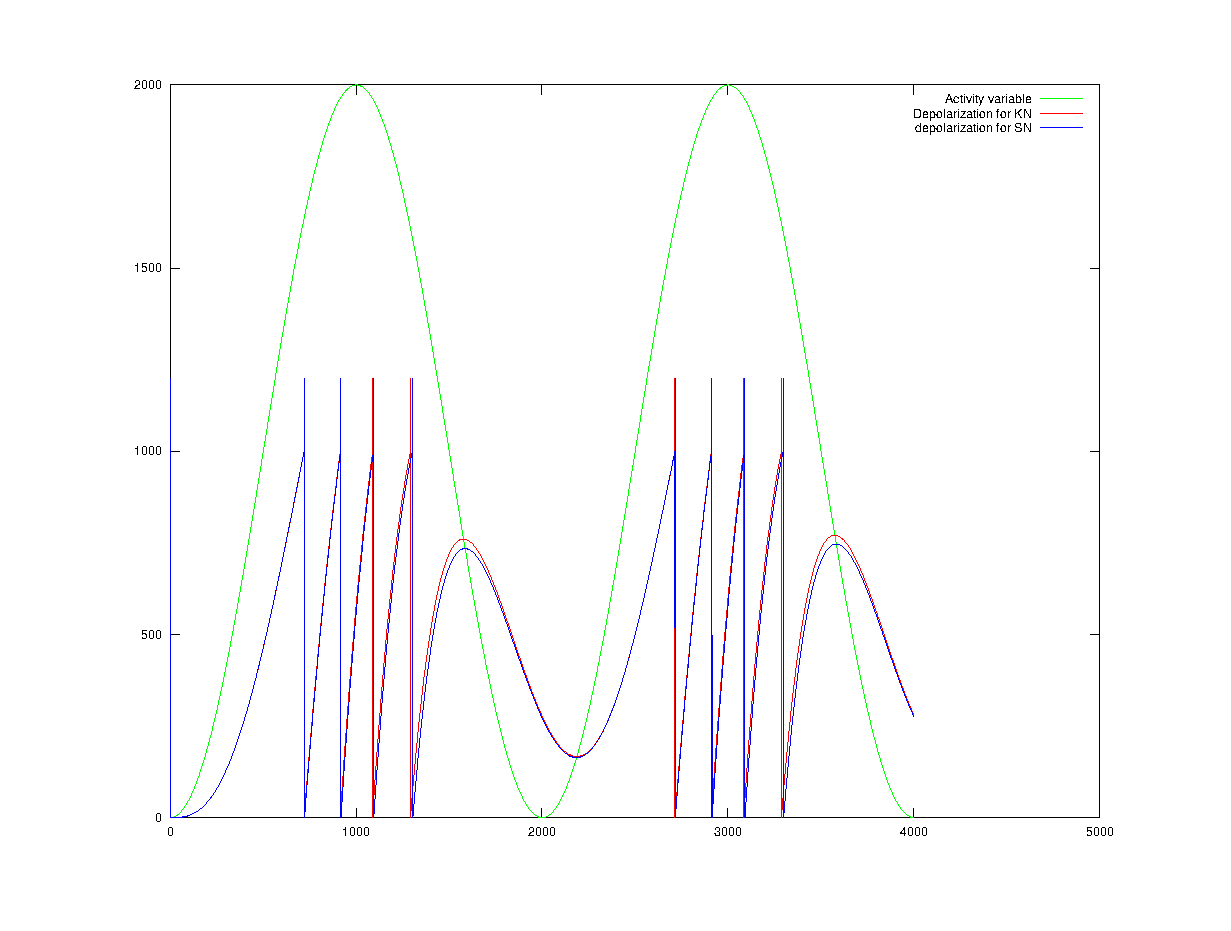
\includegraphics[width=0.95\textwidth]{eps_Comparison_between_the_two_sensors__depol.eps}
	%\end{center}
	\caption{The depolarization curve for a SANN node and a $\kappa$ANN node with the same input. The sensor function is also plotted in green for the analysis of the result.}
	\label{figComparisonBetweenSsensorAndKsensorDepolCurve}
\end{figure}

%The sensor function used for the comparison of the time course of the depolarization of a single node is 
The sensor function used in fig. \ref{figComparisonBetweenSsensorAndKsensorDepolCurve} has the formula \mbox{$f(t) = \tau (1 + cos( \frac{\pi \, t}{1000} ))$}, where $\tau$ is the firing threshold for the neuron. 
The activity variable of the K\_sensor\_auron is set to the value of the sensor funciton every time we iterate time. %XXX i time_class::doTask() Skriv litt meir. 
%For the K\_auron the activity variable is at each time step set to this variable. 
When \emph{time\_class::doTask()} updates the K\_sensor\_auron's activation level, this is done by updating the ``input'' to the dendrite.
%When K\_sensor\_auron changes its activation level, we do this by sending the sensed signal to the dendrite. 
%TODO Neste linje: referer (cite) eller internreferer til annen plass i teksten. Trur det er best å CITE.
This is very simular to the mechanisms of a sensor neuron in biology. %Evt kan eg skrive at "this is strongly inspired by nature".
%referer.
%Beste for refereringa over er nok å skrive om dette i BiologiskeSystemer.tex, og referere til plassen det står. 

%TODO Skriv ENTEN forrige linje ELLER neste greiene. NO: Repeterer meg sjølv! XXX
This implementation is strongly inspired by the biological neural system, and the stimuli is sent to the dendrite as any synaptic input.
For the K\_sensor\_auron this gives the code
%TODO Vær sikker på at dLastSensedValue = dSensedValue; dSensedValue = (*pSensorFunction)();
% Først i koden, under.
%ELLER kanskje heller: skriv om changeKappa_abs() ?!?
\begin{lstlisting}
dLastSensedValue = dSensedValue;
dSensedValue = (*pSensorFunction)();

changeKappa( dSensedValue - dLastSensedValue ); 
\end{lstlisting} %Eller så kan vi gjøre det direkte. (sette Kappa til målt verdi. har impa begge..)
and for the s\_auron we have %TODO BLI HEILT SIKKER PÅ ALPHA. Sjekk om det fortsatt er som under, eller om dette har blitt tatt inn i s_dendrite::newSignal() XXX
\begin{lstlisting}
pInputDendrite->newInputSignal( (*pSensorFunction)() );  
\end{lstlisting} % TODO Forstå greia med ALPHA! (er der fortsatt slik at eg sender inn
							% pInputDendrite->newInputSignal( (*pSensorFunction)() * ALPHA );   XXX ?


Because of the mechanisms implemented for synaptic transmission in $\kappa$ANN is based on the derived, we change $\kappa$ by the discrete variant of the derived; 
The current sensed value minus the last sensed value.% or dSensedValue - dLastSensedValue.
For the s\_auron we incoorporate the time constant T as $\frac{1}{T} = \alpha$ %eller :  $.. = $ ALPHA 
		by sending the above listed input to the s\_sensor\_auron's dendrite.


In figure \ref{figComparisonBetweenSsensorAndKsensorDepolCurve} we can se the results. 
As can be seen, the depolarization of the K\_auron and the s\_auron is quite simular.
There is a small difference between the curves.
%It is hard to know the specific reason for the error in this implementation.  In the following section I will discuss possible explanations.

What is interesting about this curve is that it seems that the depolarization curves follow eachother exactly %Dette er rett stavemåte: exactly (google translate)
for the rising phase of the sensor curve. For the falling phase of the curve we get some difference between the depolarization of the SN and the $\kappa$N.

% Skrive at for SANN så:
For discrete integration we may get something called the trunctation error. The ``local truncation error'' is the immediate error after each time step. 
The ``global truncation error'' is the error following integration multiple local truncation errors. %eller "many truncation errors", eller noke anna? (kan bli for pent språk også!)
The global truncation error is defined as the absolute difference between the approximated solution and the actual solution. 
For the SN this might become a problem, and could be the basis of the difference of the simulated node's depolarization.%Skriv om. XXX

% TODO TODO TODO Skriv også at denne "truncation error" er tatt hand om i KANN, og bude vore minimal. For SANN er ikkje dette mulig (Ingen mulighet å rekalulere verdien).
%  					XXX Dette er veldig viktig poeng for seinere analyse av KANN vs. SANN!

\subsubsection{Trunctation error of the SN} %Kanskje skrive "Spiking Node". Hugs at overskrifta blir også oppført i "index".
In SANN each node is modelled as a leaky-integrate-and-fire neuron.
When the depolarization of the SN is updated, the leak of the neuron calculated as the previous value times the leak constant.
The updated value then becomes %todo Skriv om denne setninga.
\begin{equation} %TODO Introduser denne ligninga tidligare i oppgava. Her skal eg bare skrive siste del av den:    v_t = (1-\alpha) * v_{t-1}  XXX HAR EG GJORT DET? TODO SJEKK!
	v_t =  (1-\alpha) * v_{t-1}  
\end{equation}
%TODO Skriv om: krøtkete måte med/mellom alle komma'ane.
The discretization of the system introduces a small error, the local truncation error, that varies with the size of the time step and the derived of the value function $\dot{v}(t)$. %"local truncation error"

The leak is calculated as the $-\alpha v_{t-1}$.
% Skriv at når feilen oppstår, så er dot(v(t)) positiv, dette gir:
When $\dot{v}(t)$ is positive, $v_{t-1}$ is less than the value $v_t$, varying with the size of the time step and the differentiated value function $\dot{v}(t)$.
When $\dot{v}(t)$ is negative, we get the oposite result.
%skriv at dette nuller ut problemet. (MEN (det kommer at) siden det alltid fyrer etter positiv flanke, blir det integral av en liten integralfeil ved kvar fyring. XXX Viktig poeng. Sjekk at det er stort nok skrevet lenger nede.

Each small error is integrated up to a larger error, the global trunction error. 
If some situation is analyzed where the value is the same as the initial value, the integral of the derived over this interval is per definition zero.
Global trunctation error will then dissapear. 
This further implies that for a continous signal that varies around some working point, the global trunctation error will not diverge.  %google sa at det heite "diverge"

\begin{figure}[hbt!]
	\centering
	%\begin{center}
		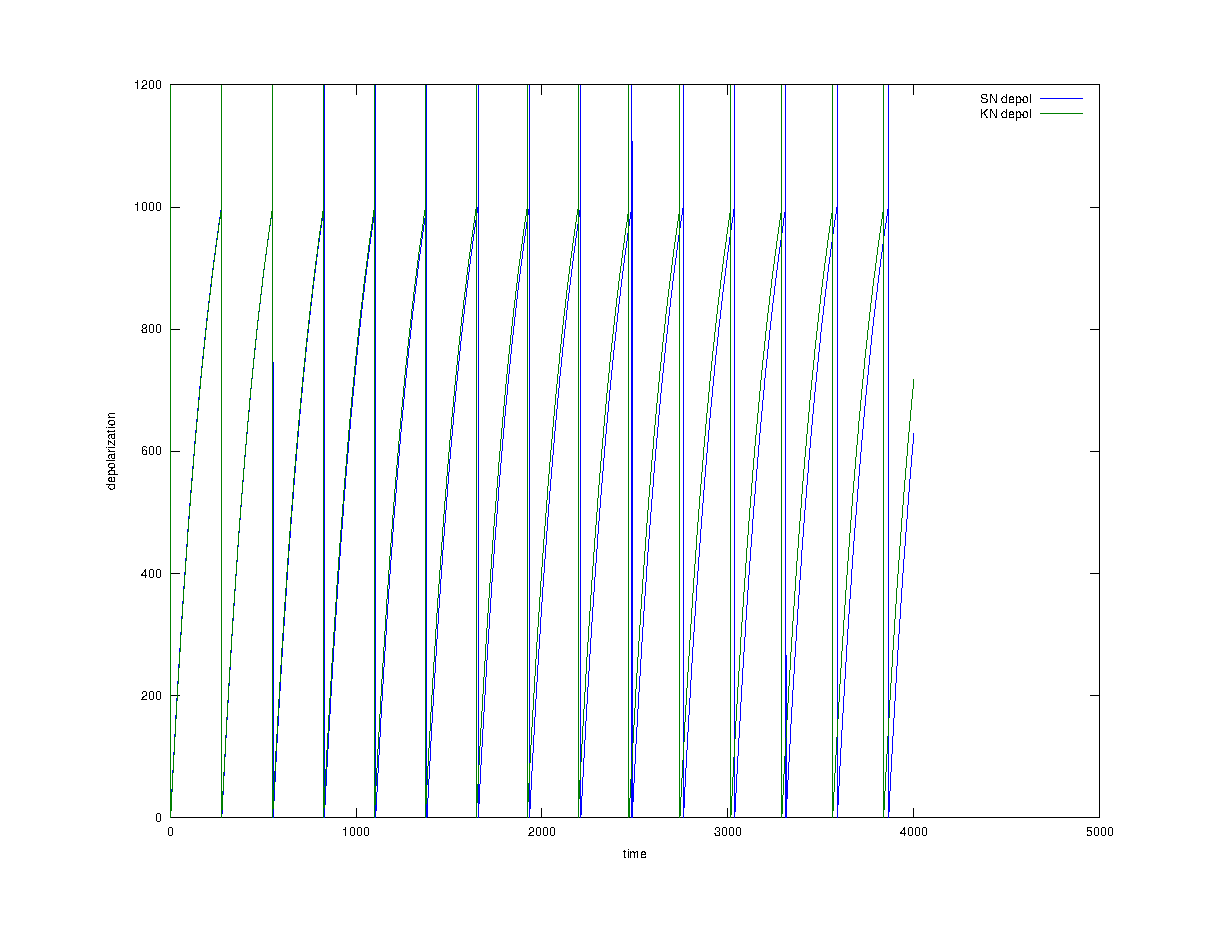
\includegraphics[width=0.95\textwidth]{eps_comparison_between_KN_and_SN_ConstKappa.eps}
	%\end{center}
	\caption{The depolarization curve for a SANN node and a $\kappa$ANN node with the same input. The sensor function has an input equivalent to an activation level of $\kappa = 1.5 \tau$ for both nodes.} %XXX Eller for begge nodeModeller
	\label{figComparisonBetweenSsensorAndKsensorDepolCurveCONStActivityLevel}
\end{figure}

The depolarization of a neuron have a discontinuity when the neuron fires an action potential. 
When the neurons depolarization reaches the firing threshold the value is reset to $v_0 = 0$.
In other words, each time the value of a node reaches a positive threshold, the value is reset.
In this case the global trunctation error will continue to grow, and the difference between the value curves for the SN and the $\kappa$N continues to grow. %TODO Ikkje dette. Skriv heller eit utfall som Stavdahl vil syns er SKUMMELT!

To se if this is the backgound for the error, we isolate the error by giving the sensor aurons a constant sensor function, with an activation level of $\kappa = 1.5 \tau$.

The result is presented in fig. \ref{figComparisonBetweenSsensorAndKsensorDepolCurveCONStActivityLevel}. % .eps
If the previous analysis of the problem is sound, the SN should have a depolarization that is higher than is should be.
This implies than the depolarization curve for the SN would be ``before'' that of the $\kappa$N, which is the opposite of the situation of fig. \ref{figComparisonBetweenSsensorAndKsensorDepolCurveCONStActivityLevel}.

\subsubsection{Rounding errors}
%TODO Skriv om: Ikkje røp løysing først. La det være litt spenning!
After a more thorough analysis of the error, it seems that the difference is an effect of a rounding error.

If we change wievpoint on the error and see the difference between the two cuves as an effect of time, we can say that the $\kappa$N's depolarization curve lies before the SN's depolarization curve.
This implies that the $\kappa$N fires before the SN, and thus starts earlier on the depolarization for the next period.

In many programming languages a float is always ``rounded down''. This means that the DECIMAL %XXX FINN RETT ORD: Det som står etter komma TODO
	is removed from the number, and the integer becomes the same as the integer part of the number.

%TODO Viktig: Hugs å skrive om kvifor eg valte en mindre periode i starten av sensor-funk. Dette er viktig, ellers trur han nok at eg bruker dette for å skjule feilen..
\begin{figure}[hb!tp]
	\centering
		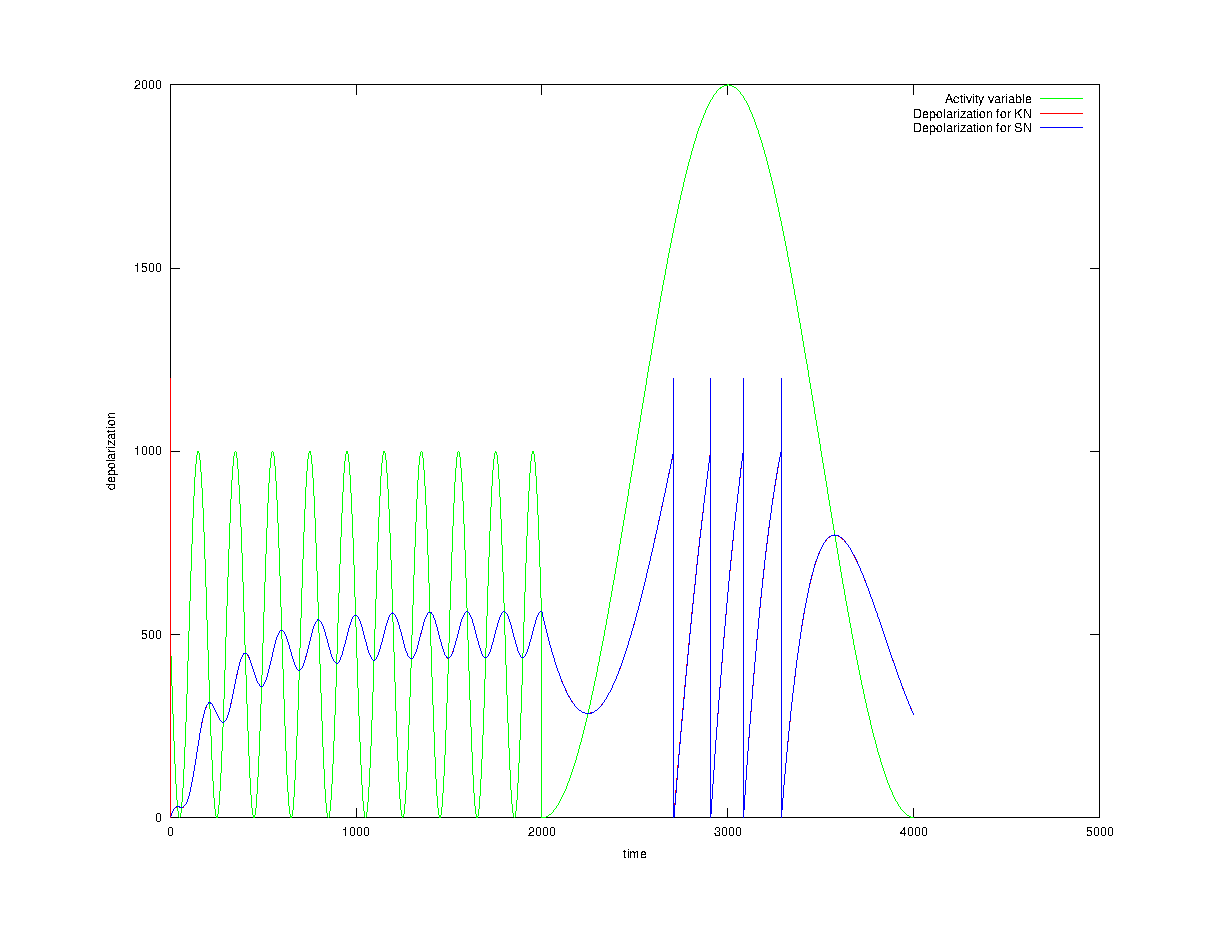
\includegraphics[width=0.95\textwidth]{eps_Comparison_between_the_two_sensors__depol_FIKSA.eps}
	\caption{Comparison between the SN's and $\kappa$N's depolarization curve. The sensor function is plotted in green for analysis purposes.}
	\label{figComparisonBetweenSsensorAndKsensorDepolCurveFIXEdError}
\end{figure}

When the $\kappa$N calculates the estimated firing time, this calculation is done in a double precision floating point number. 
To use this in the scheduler is must first be transformed to an integer variable. When this time step arrives, the task is executed.

%TODO Skriv at vi vil heller runde til nermeste integer, opp om det er best.
% Så skriv korleis dette gjøres, så finn rett kurve.
% TODO analyser frem og tilbake om kor feilen ligger. Det er fortsatt mulig at feilen er for KANN (men trur ikkje det. Legg at feilen er maks når subthreshold polarization er størst. Osv.) XXX
If we instead round to the closest integer, by adding $0.5$ to the float before it is converted into an integer, we get the depolarization curve presented in fig. \ref{figComparisonBetweenSsensorAndKsensorDepolCurveFIXEdError}.
In the improved depolarization curves for the auron, the error is small and can not be seen on the plot.

%Ikkje heilt sikker på om det er heilt rett: størst etter "rising flank of the ..", Bli heilt sikker på dette.
The error is found to be largest right after the rising flank of the activity variable's curve. %TODO ta vekk:   [ , the value of the sensor function. ] ?
For the situation in fig. \ref{figComparisonBetweenSsensorAndKsensorDepolCurveFIXEdError} this is at time t=3000.
At this time iteration the value of the SN is 1.015 more than the value of the $\kappa$N. 

This deviation is substantially smaller that the deviation originating from the rounding error, but it indicates that the analysis made in the previous subsection is correct. %gjør om: ikkje "correct" men kanskje mindre påståelig?
%TODO Skriv analyse av denne feilen, og peik på mulige scenarioer.


% TODO KANSKJE :   \subsection{Floating point calculation pitfalls}
%                  Skriv om mulighetene for feil når man bruker float/double.


% - integralfeil for SN
% - Integralfeilen kommer antagelig av at lekkasjen  
% - For SN vil lekkasjen regnes ut fra verdien ved forrige tissteg. Denne diskretiseringseffekten vil forplante seg i at for positiv derivert av depol-kurva vil SN-depol være litt over, og for negativ flanke : motsatt.
% 		Dette er fordi lekkasjen regnes ut fra forrige verdi, som for stigende flanke er mindre enn den noværande verdien, og vi får en mindre lekkasje => for stor verdi.
% - denne feilen vil nulles ut for eit periodisk signal uten sprang (over en periode vil integralet av positiv flanke og neg. flanke bli null.
% - dersom vi har eit sprang, eller enda verre: eit sprang som alltid ligger etter en viss mengde med pos. flanke, vil vi få summert opp integral-feilen.
% For auronet vil depol settes lik 0 etter en viss mendge pos. flanke for depol. kurva. Dette skaper problemet.

% Eg har også vurdert om det er feil fra implemenasjonen: at de har ulik refraction time, MEN eg trur ikkje dette: 
% 		En slik feil ville vore mindre (eit-to tidssteg per fyring) => ikkje synlig på eit plott over fleire tusen iter's.


% MEN PROBLEMET ER FEIL VEI! JEje. Drit i det!




% Den lille forskjellen mellom s_sensor_auron og K_sensor_auron er noko eg kan skrive mykje om i 'discussion'.
% Eg har tanker om at det er pga. at eg bruker integer (tid) i ligningene, og vi får dermed avrundingsfeil. Litt overraska over at feilen er så liten..
% 	Det er også mulig at den lille forskjellen kommer av forskellane i korleis sensor-funksjonen blir oversatt til depol.
% 		- K_sensor_auron oversetter sensorFunk direkte til aktivitetsVariabel Kappa, mens
% 		- s_sensor_auron sender gir eit enkelt input per tidsiterasjon gitt av ligninga (W_ij / [time constant]), eller  ALPHA * W_ij
%   XXX Dette trenger grundigare analyser!





%XXX Skriv i conclusion:
%Because a network of connected neurons have a large degree of complexity, it is best to start with comparing the depolarization of single nodes.
%For comparison of the two models, we will first compare the depolarization of a single neuron of each model.
%Because a system comprised of a network of neurons have 


\section{Resultat for effektivitetssammenligning}



\section{Discussion}
In the course of this project new model for artificial neural networks have been developed. 
Because the primary focus of the project was to compare a new model for ANN with the ability to represent both firing time and firing frequency, with the SANN model, the development and implementation recieved this focus. 
The new model is therefore implemented as a mere variant of a third generation ANN.
%XXX Kanskje eg overdriver kor liten eg har gjort den :  "... mere variant of ..." Skriv litt mindre høg på pæra?

If we define the third generation ANN as a network of nodes capable of integrating the input to a state for the node, and this state gives the firing time of the node, it is possible to place $\kappa$ANN in this group.
The output of each node in $\kappa$ANN could be defined to be the spikes after a sufficient input to the node.
In this case the ANN becomes a Mealey automata of the SANN model. This is how it is implemented in this project.

If we instead let each $\kappa$N give an output as a function of the present and estimated future input, and give a similar output, the network becomes something else.
The output now varies as a function of the input, and the node becomes stateless in this respect. If desired, the spike time and state of the neuron can still be calculated. 
If the third generation ANN is defined as a network of nodes that gives output as a function of the nodes value, $\kappa$ANN therefore falls outside this group.

In this implementation, it is possible that the full advantage of the new model is neglected in the desire to compare the model to the SANN model.
Because this was first discovered when the results were analyzed, and due to little time, this will be placed under "for furter work". % TODO TA vekk/SKriv om!
%FORTSETT HER!

%så gå over til sammenligning av denne mot SANN.


\section{Discussion 2. Denne skal nok vekk.}

% TODO TODO TODO TODO TODO TODO TODO TODO TODO TODO TODO TODO TODO TODO TODO TODO TODO TODO TODO TODO TODO TODO TODO TODO TODO TODO TODO TODO TODO TODO TODO TODO TODO 
% DETTE er ikkje diskussjon. Dette er implementasjon eller noke. Finn ny plass!
% TODO TODO TODO TODO TODO TODO TODO TODO TODO TODO TODO TODO TODO TODO TODO TODO TODO TODO TODO TODO TODO TODO TODO TODO TODO TODO TODO TODO TODO TODO TODO TODO TODO 

%En eller anna plass: (ikkje akkurat her) Skriver her fordi eg har inspirasjon no, og ikkje vil leite..) 	Ja! Kanskje i "conclutions"XXX
Implementing the mechanisms of a neural simulator is not trivial, even without optimizing it for run time efficiency.
%todo SKriv om neste linje! xxx
Even if this is not an important aspect of this project I have tried to, wherever possible, optimize the implementation for efficiency.
%Skrive kvifor: Om at designet er optimalisert både for generalitet (for å gjøre utvidelser/endring lettere) og for effektivitet. DETTE for å kunne bruke implementationen videre (personlig, eller for andre).

The functions that are most often called are inlined. This means that I have given a hint to the compiler to put the compiled code wherever the functions are called.
This causes the function calls to run faster but also increases the size of the executable file, so this should be used with caution. %Kanskje skrive dette, men også da skrive størrelse på endelig program. ca. 0.5 M (?)
For this implementation, size will not be a problem. %Kvifor?
Inlining of functions are still kept to a minimum, in case of further work on this software. %skriv annaleis. Kvifor "in case of further work on this software."? Forklar bedre, eller skriv om (anna argumentering).

Also in other parts of the implementation, the code is written with a focus on possible future expantion.
%Difor er ting laga enkel å forstå for en som kan nevro: oppsettet av nodene er lagt opp som det biologiske neuronet.
The object model is designed to be general for the two models, both to make the two implementations more comparable for this project and to make the implementation better suitable for future comparison.

The design of each node is based on the biological neuron to be more intuitive for programmers with knowledge of neuroscience. 
This is not only to make the implementation easier to use for potential future programmers, but also because little is known about what is important in neuroscience.
If the implementation is constructed strongly inspired by the emulated system, with multible elements constructed in the same way as the original system, expantion and modification of the indivitual elements involve less effort.
Say, for example, that new aspects are discovered tomorrow. In this case, the code can easier be modified after this discovery.

This principle does not only account for future uses by other programmers.
In multiple occations, aspects that are where new to me have been implemented at after the main functionality of the classes where designed. 
This required less work because I followed principles that was important to Bjarne Stroustrup during the creation of C++; To make the design general and open and suited for any future uses.%ELLER NOKE Siter"TheDesignAndEvolution of C++".


% TODO TODO TODO TODO TODO TODO TODO TODO TODO TODO TODO TODO TODO TODO TODO TODO TODO TODO TODO TODO TODO TODO TODO TODO TODO TODO TODO TODO TODO TODO TODO TODO TODO 
% dette ER diskurs (?) :
One element that is not implemented, is axo--somatic and axo--axonic synases. 
This is synapses where the input to the postsynaptic neuron enters at other places of the neuron than the dendrite. 
In biology, most inhibitory synases have theire input close to the soma of the postsynaptic neuron. 
This will give the inhibitory input less delay compared to the exitatory input, and might be an important aspect in neural computations.
This can be implemented easily if this is found to be important for some future use of this code.

An other important aspect that is not impelented is axo-axonic synapses, linked to short term synaptic plasticity.
%XXX An axo--axonic synapse is a synase that enters the postsynaptic neuron somewhere close to one of its output synapses.
% Gjør om rekkefølgen litt. Skriv om short-term syn.p. først, så evt. axo-axonic synapses.
Short--term synaptic plasticity is synaptic plasticity that does not have any long term effect of the neuroal network (learning), only on more immedate aspects of signal transmission.
In particular, we have the synapses that gives input near the axon terminal of the neuron (axo-axonic synapses). This will alter the depolarization at the neurons output synapses. %og auke/minke mengde Ca2+ i presyn. bit av synapsen.
This will not cause any transmission to occur, only ``prime'' the presynaptic membrane of the synapse for transmission.
When the next action potential arrives, the size of the transmission will be larger than usual (or less, depending on whether the axo--axonic synapse is exitatory or inhibitory).
Again, neither short--term synaptic plasticity or axo--axonic synapses has been implemented because this was not an aspect of this project and due to time constraints.
% Skriv heller at short--term syn.p. ikkje er implementert, så axo-axonic synapses ville ikkje auka funksjonaliteten til simulatoren.
Implementing it will involve less work due to the implementation design in this code.
% Denne setninga er for å vise at det er lett å innføre. Skriv om.

If the goal of the implementation is to simulate a neural network from biology, spatial and temporal resolution is more important than efficiency of the calculation.
%When it comes to temporal and spatial resolution, this can easily be extended.
In this implementation, spatial and temporal resolution can easity be extended.
If we want to increase the accuracy, this can be done by increasing the number of elements in each node (and making the timestep accordingly smaller).
This will also make the computational efficiency of the simulator less, and the pragmatic use of the simulator will suffer.

If we need a better accuracy, and for example double the number of serial elements in each node and halve the size of the timestep, the functioning of each element will be the same.
The temporal and spatial resolution will be increased two-fold at the expence of the computational efficiency of the simulator.

With ``spatial resolution'' i refer to the ability to separate between elements located at different positions in space.
This is important for the output, scince different output synapses are situated at different locations of the neurons axon.
This will cause different transmission delays, and might be important for the neural calculations.
% Also the axon will be have more elements, and different synapses along the axon may have differenti time delay.
This gives us the ability to make a separation between ``early synapses'' and ``late synapses'' along the axon, and gives us a better spatial resolution for the simulated neuron.

The whole reason for developing the third generation ANN, spiking artificial neural networks, was the growing focus on the timing of the different events within the neural network.
This is computational demanding, and high resolution simulations is not suited for real time pragmatic uses of ANNs. For simulations used to test hypothesis in neural science, however, accuracy is most important.
The focus on generality in this implementation will therefore make the code reusable for possible future pragmatic uses and for implementing neural simulators.

If the new model is more effective than the old model for spiking neural networks, we can not know whether this is only goes for one of these uses. 
For this reason I found it best to implement as generally as possible, for future efficiancy comparison between the two models.
%Skrive eksempel: "More specifically, if we divide the axon into smaller pieces, spatial accuracy is better."
%Skriv om forskjellane mellom KANN og SANN. Her kommer kanskje største fordelen med KANN? (Kan kanskje legge inn vilkårlig antall element, til tilsvarende størrelse på 'time step').

%slutt: En eller anna plass: ....


\section{Conclution}
% DET neste er ikkje bra å ha her!
Grunnen for å fokusere på spike time, i utgangspunktet var oppdagelsen av at synapser lærer ved positiv eller negativ vekt-endring etter overføring. 
Hvilken, og kva størrelse er avgjort av når synaptisk overføring kommer i forhold til postsyn. fyring.

Etter litt har man funnet ut at desse mekanismene bare gjelder enkelte synapser, der postsynaptiske neurotransmittor receptors er spenningsavhengig for overføring. 
Med høg depolarisering, dvs lav spenning overføres meir, og bl.a. $Ca^{2+}$ som er viktig for postsynaptisk plastisitet.
"To my knowledge" har det bare blitt funnet en slik neurotransmittor-sensor i biologien. Dette er den glutamatiske NMDA receptoren.
Glutamatisk overføring har vore veldig mykje i fokus for synaptisk overføring, og det er ikkje rart at STDP har fått så veldig høgt fokus %NEI, FAEN! må ikkje argumentere mot oppgaveteksten!


\section{Notater: Kva burde eg gjordt annaleis?}
Burde ikkje bygd de to implementasjonane så lik. (?)
Det er vanskelig å sammenligne de to. For K\_auron kunne eg ivertfall droppa dendrite og kanskje axon.
Jeje - vettafaen eg.

Burde ikkje brukt så mykje tid på pEstimatedTaskTime-lista. Kanskje eg kan argumentere for at dette kan være nyttig, men for dette prosjektet er det tidssløs.


\section{Ting som kanskje er nye}
Skriv litt om optimaliseringa gjordt i SANN. Simulert asynkron tid istedetfor oppdatering kvart tidssteg.

Kalkulering av lekkasje: Kvar gang det kommer nytt input, framfor å gjøre det kvar tidsiterasjon.

\section{Kva burde eg gjordt annerledes?}
Skriv at fokuset mitt i denne implementeringa var å sammenligne de to modellene. Dette gjorde at eg satt opp auronet på eg spesiell, og ikkje-optimal måte.
(Både for effektivitet, men også for implementasjon. Det var kanskje vanskeligere å implementere modellen på måten eg gjorde det, enn nødvendig. Kann trenger bare eit auron, med synapser ut.)
Dette burde eg gjordt annerledes, og både implementering og effektivitet ville vunnet på dette.



% XXX Skriv at resetting til v_r etter AP er ikkje instantaneous. Dette tar også litt tid. For videre arbeid vil også dette bli implementert!

% XXX Skriv at KANN er en mellomting mellom fANN og SANN. Det har muligheten til å kommunisere med begge.
% 		- fANN kan overføre aktivitetsnivået sitt direkte til KANN (Kan sette $\kappa$ = input-fra-fANN) -- Begge veier (KANN: kan få info FRA, og gi info TIL fANN).
% 		- SANN kan overføre aktivitetsnivået sitt indirekte til KANN (KN kann analysere input til $\kappa$. KN kan gi output til SN (direkte))
% Det kan være dette er eit stort bidrag for ANN-verden. Dersom det i tillegg er meir effektivt, så ...



%legg meir?



%\appendix %Unødvendig å skrive. Bare for å gjøre det synlig.. (makroen er kalla i appendixSynPlast.tex)
% XXX XXX XXX XXX XXX XXX
% 		APPENDIX 
% XXX XXX XXX XXX XXX XXX 
%Kanskje eg skal ha med "table of abbrevations" i appendix, eller først.
%TODO include{appendixTableOfAbbrevations} , eller ha det før innledning..


%TODO TODO TODO TODO TODO TODO TODO TODO TODO TODO TODO TODO TODO TODO TODO TODO TODO TODO TODO TODO TODO TODO TODO 
% 
% 	KVA må være med i dette appendix: (ting som eg har referert hit, for meir info):
%
% 		- short--term synaptic plasticity som en konsekvens av raske overføinger (potentiation).
%
%TODO TODO TODO TODO TODO TODO TODO TODO TODO TODO TODO TODO TODO TODO TODO TODO TODO TODO TODO TODO TODO TODO TODO 








%Seier fra til tex at resten (eller neste) skal være nummerert som appendix (i referanser og i index):
\appendix
\chapter{Synaptic Transmission and Plasticity in the Biological Neuron} %xxx Eller biologisk neurale sys. (er vel strengt tatt ikkje i nevronet, ELLER er det det?)


%fra NEVR3001 rapport om synPlast : (Kraftig omskrevet)

%\section{Introduction}
\label{appendixSynPlast}

The background of memory and learning is an important topic in the field of neuroscience. 
It has recieved much attention lately, and the knowledge about synaptic plasticity and synaptic transmission has progressed significantly the last decades.
In this appendix the different mechanisms behind synaptic transmission and plasticity will be in focus.
We will see that the the ion $Ca^{2+}$ has a crusial role in both presynaptic transmission mechanisms and in postsynaptic mechanisms involved in synaptic plasticity.

% todo Ta vekk (Skreiv det bare inn for å forklare en kybb-leser. Trur syn.p. er kjendt etter rapporten min).
%First some expressions will have to be defined. Synaptic plasticity referst to change in the size of each of the synapse's transmissions.
%Synaptic plasticity may be short--term, lasting from milliseconds to minites %TODO finn ut kva noken seier, og referer dette (Bear, purves, kandel)
% 	, or long--term, giving us ``memories'' that might last from hours to a lifetime.

Synaptic transmission in chemical synapses is dependent on a multitude of different mechanisms situated in the presynaptic axon terminal, the postsynaptic membrane or in glial cells surrounding the synapse.
%Synaptic transmission in chemical synapses is based on many mechanisms both in the presynaptic axon terminal, the postsynaptic neuron, and in glial cell surrounding the synapse.
Some of these mechanisms involved in synaptic transmission will be discussed in this appendix.
We will also look at some elements involved in synaptic plasticity, or change in the size of the synaptic transmission. %TODO Skriv kvifor? FÅ RELEVANS!
% TODO Skriv noke slikt som: Because the ultimate goal of this appendix is to discuss the reason behind going on from
% XXX 	og end opp på at eg må beskrive syn.p. også.
% xxx  	Kan kanskje bare skrive at desse er tett sammenknytta. Nei, eg må forklare kvifor eg vil beskrive STDP.
%In this essay, some of the mechanisms involved in synaptic transmission will be described. 
%This is nessecary in order to say something of what changes the same mechanisms.


%Innleder synaptic transmission:
When the neuron is sufficiently depolarized, an action potential is initiated at the axon hillock.
The action potential will propagate through the axon to the ``axon terminal'' where the presynaptic part of the synapse is found.
When we get a strong depolarization over the presynaptic membrane at the synapse, a cascade that ends up with a change in the postsynaptic neurons value is initiated.
This is what is referred to as synaptic transmission\ref{PurvesNeuroscienceKAP05}.

The size of the synaptic transmission is dependent on the amound of neurotransmitters released from the presynaptic part of the synapse and the number of neurotransmitter resceptors in the postsynaptic membrane
		\ref{PurvesNeuroscienceKAP05}. 
Synaptic plasticity, what is percieved as the basis of learning, can happen on a short--term of long--term timescale.
Short--term synaptic plasticity normally only involves factors that can be seen as ``the state'' of the synapse. 
Factors as neuromodulators, amount of $Ca^{2+}$ in-- or outside the neuron and amount of neurotransmitters available are examples of such factors.
Long--term synaptic plasticity involves ``lasting changes'' in the synapse. One example is such protein synthesis is generation of new postsynaptic receptors\ref{PurvesNeuroscienceKAP8}. %todo har ikkje sett gjennom kap.8 når eg ref.
																										% Veit innholdet, men det er kanskje lurt å sjekke at alle desse elementa stå i purves kap 8.

\section{The presynaptic part of synaptic transmission}
\label{appendixSecPresynapticSynapticPartOfTransmission}
The propagation of the action potential along the axon, happens as a combination of passive and active transmission.
The electrical potential is transmitted passively along the axon. On the axon we have voltage--gated $Na^+$ and $K^+$ channels.
These will open when the electrical membrane potential supasses a threshold, and will further increase the value of the potential. 
After a while the channels will close in a sequence that resets the potential to the base potential (with a small overshoot) \cite{PrinciplesOfNeuralScience4edKAP09}. 
%and will not activate reamplification before it encounters special voltage--gated $Na^+$ and $K^+$ channels.
%The axon is insulated by a special glia cell, to increase the speed of action potential propagation.
%These are situated in gaps in the insulation, or glia
This will reamplify the signal  so that is may continue passively down the axon to the next voltage gated channels.
%In an action potential, electrical potential is first transmitted passively down the axon of a neuron. On the axon we have voltage--gated $Na^+$ and $K^+$ channels 
%	that open when the electrical potential over the membrane surpasses a threshold\cite{PrinciplesOfNeuralScience4edKAP09}. 
%This will enhance the signal so that it can continue passively to the next voltage gated channels.

In the nervous system we have specialized insulative cells, called myelin.
In myelinated neurons, the voltage--gated channels are located in gaps in the myelin, These gaps are called ``nodes of Ranvier''.
%skriv også om situasjonen for umyeliniserte axon? Nei.
The voltage--gated channels will restore the action potential, and constitutes the active element of signal tranmission along the axon \cite{PrinciplesOfNeuralScience4edKAP09}.
%In myelinated neurons these voltage--gated channels are located in gaps in the myelin, called ``nodes of Ranvier'', in unmyelinated neurons the channels are located continously along the axon membrane. The channels will restore the signal, and constitutes the active part of current transduction along the axon\cite{PrinciplesOfNeuralScience4edKAP09}.


%*********************** OK så langt. ***********************

When the action potential reaches the axon terminal, the end of the axon down the signal path, it will open voltage gated $Ca^{2+}$ channels at the active zones of the terminal. 
This causes $Ca^{2+}$ to enter the cytosol of the axon terminal of the presynaptic neuron\cite{PrinciplesOfNeuralScience4edKAP10}.

$Ca^{2+}$ causes synaptic vesicles to fuse with the membrane and release the contained neurotransmitters into the synaptic cleft.%\cite{PrinciplesOfNeuralScience4edKAP10}. 
There is a linear relationship between the amount of $Ca^{2+}$ entering the cytosol and the amount of synaptic vesicles fusing with the membrane (exocytosis).%\cite{PrinciplesOfNeuralScience4edKAP10}. 
Ecocytosis of a synaptic vesicle will release the neurotransmitters stored in it into the synaptic cleft \cite{PrinciplesOfNeuralScience4edKAP10}. 
The amount of neurotransmitters released into the synaptic cleft therefore have a linear relationship with the amount of $Ca^{2+}$ entering the presynaptic axon terminal.
% TODO Ta med, eller ta vekk?      , given a constant amount of neurotransmitters stored in each synaptic vesicle.
%Exocytosis releases the content of the synaptic vesicle to the synaptic cleft\cite{PrinciplesOfNeuralScience4edKAP10}.

%XXX Viktig, men utafor scope av teksten:
%%%%%%The linear relation between the amount of $Ca^{2+}$ entering the axon terminal and the amount of synaptic vesicles undergoing excytosis was first proposed by Katz and Miledi, and later shown by Rodolfo Llinàs and colleges\cite{PrinciplesOfNeuralScience4edKAP14}. 
%KANSKJE:
% TODO Vettafaen om det skal være med:
% Dette gir at vi kan ha presynaptisk short--term syn.p., noke som er viktig argument for å innføre axo-axonic synapses (temporal synaptic modulatory system)
%Rodolfo Llinàs and colleges first showed the mechanisms of a linear relationship between the amount of $Ca^{2+}$ entering the cytosol of the presynaptic cytosol.
%They also found that the $Ca^{2+}$ channels are graded by the potential over the axon terminal membrane. 
%This further gives a graded responce of neurotransmitter release based on the preysnaptic membrane potential \cite{PrinciplesOfNeuralScience4edKAP14}.
%xxx kan ikkje ta vekk, lett. Bruker dette resultatet seinere.. ELLER?

% TODO Flytt alle \cite{} til slutten av avsnittet (dersom de påstandene på slutten også står her..)
% Har sjekka: alle påstandene er fra kap14 i Kandel.
There is a steady influx of $Ca^{2+}$ at axon terminals, through the L-type $Ca^{2+}$ channel. %\cite{PrinciplesOfNeuralScience4edKAP14}. 
This influx of calcium is graded by the potential over the presynaptic membrane.
When multiple synaptic transmissions happens within a short period of time, 
	the amount of $Ca^{2+}$ in the presynaptic axon terminal builds up and the following synaptic transmissions will give a successively larger effect on the postsynaptic potential.
This effect is called \emph{potentiation}, and can last from minites to more than an hour.
% Føler at neste linja ikkje heilt passer inn XXX:
% TODO Vær sikker på at axo--axonic synases er definert!
This mechanism also gives the effect of axo-axonic synapses in regulating the amount of neurotransmitter release for the next transmissions\cite{PrinciplesOfNeuralScience4edKAP14}.
%The axo-axonic synapses will not influence the firing of a neuron, only the membrane potential of the an axon terminal. %XXX KVA ER axo--axonic synapses? Inled dette for leser!
% % and thus the amount of neurotransmittors released by the following action potential\cite{PrinciplesOfNeuralScience4edKAP12}.
%This gives a mechanism for controling the postsynaptic exitatory postsynaptic potential between other neurons following an action potential.

%TODO TA vekk?
%When two action potentials reaches the axon terminal in fast succession it will cause the synapse to be stronger (give a larger postsynaptic response) for many minutes. 
%This is called \emph{potentiation}, and is thought to be partially because of the increase in presynaptic cytosol $Ca^{2+}$ levels\cite{PrinciplesOfNeuralScience4edKAP14}. In the mossy fiber pathway of the hippocampus, presynaptic $Ca^{2+}$ influx is an important mechanism for synaptic plasticity \cite{PrinciplesOfNeuralScience4edKAP63}. %XXX Sjekk! (mest viktige, eller bare viktig?)

%XXX TA VEKK? 
%A decrease in the number of synaptic vesicles undergoing exocytocis has been observed in sensory neurons of the \emph{Aplysia Californica} following LTD. %, by quantal analysis 
%The mechanisms for decrease in synaptic vesicle exocytosis is not known\cite{PrinciplesOfNeuralScience4edKAP63}.

% dette er kanskje interresant: Det kan også være en basis for STDP.. 
% Sjå om det skal takast vekk, dagen før innlevering.
An increase in the extracellular level of glutamate has been observed after LTP in CA3 neurons. 
The mechanisms behind this is debated, but evidense has been presented of \emph{retrograde messangers} from the postsynaptic neuron that will 
	give feedback to the presynaptic neuron after transmission \cite{PrinciplesOfNeuralScience4edKAP63}. 
This enables a  presynaptic component of \emph{long--term} synaptic plasticity.








\section{Postsynaptic mechnisms of synaptic plasticity}
%There are tree groups of receptors in the postsynaptic membrane of a synapse. AMPA, .......NMDA, kainate, ....
Because neuroscience mainly have focused on excitatory glutamate synapses, the discussion about postsynaptic mechnisms behind synaptic plasticity will focus on glutamate transmission.

There are two groups of glutamate receptors: NMDA and non-NMDA receptors. 
The non-NMDA receptors consists of the AMPA and the kainate receptors. 
Most non-NMDA receptors are only permeable to $K^+$ and $Na^+$, while the NMDA receptor is permeaple to $Ca^{2+}$ in addition to $K^+$ and ${Na}^+$ \cite{PrinciplesOfNeuralScience4edKAP12}. 


The NMDA--receptor is an ion channel that is both voltage gated and ligand gated: 
	It requires both that the glutamate neurotransmitter is present in the extracellular fluid and a strong depolarization over the membrane to open \cite{PrinciplesOfNeuralScience4edKAP12}. 
When we get a transmission when the postsynaptic neuron is strongly depolarized, we therefore get an influx of calcium at the postsynaptic neuron.
$Ca^{2+}$ will activate calcium dependent enzymes and also protein kinases that leads to long--term synaptic plasticity\cite{PrinciplesOfNeuralScience4edKAP12}.
This is done as a result of the calcium dependent enzymes initiating synthesis of new AMPA receptors \cite{AMPARtrafficingArtikkel}. 
More receptors causes a larger probability of the glutamate neurotransmittor having an effect, and thus increases the effectivity of the synapse (the synaptic weight).

To conclude this section we will compare the statistical relationship between the postsynaptic neuron having a large depolarization at the time of transmission and the relative timing of the transmission, 
	in relation to the postsynaptic action potential. 
If the postsynaptic neuron is strongly depolarized at the time of transmission, this implies that the postsynaptic neuron will fire soon after.
This might be one of the basis of what has been known by the name Spike Time Dependent Plasticity (STDP).
% OMGJODT TIL HIT:  XXX XXX XXX XXX XXX XXX XXX XXX XXX XXX XXX XXX XXX XXX XXX XXX XXX XXX XXX XXX XXX XXX XXX XXX XXX XXX XXX XXX XXX XXX XXX XXX XXX 
% TODO KAnskje ta vekk resten (med unntak av Summary?)

%XXX XXX XXX XXX 
%If two transmissions happens in rapid succession, you will get a strong (lokal) depolarization around the postsynaptic receptors. This will cause the NMDA--channels to open at the second transmission, and admit $Ca^{2+}$ into the postsynaptic neuron. 
%TODO Skriv heller om at depolarisasjonen har mykje å seie. NEI, dette står allerede. Skriv korleis tid kan ha noke å seie (begrunn STDP med bakgrunn i teoien her). XXX Gjør eit poeng ut av kvifor eg har tatt med dette i appendixet.
% 			Dette kan helst gjøres etter neste setning.

%Also in the postsynaptic neuron, calcium has an important role in synaptic plasticity. 
%$Ca^{2+}$ will activate calcium dependent enzymes and also protein kinases that leads to long--term synaptic plasticity\cite{PrinciplesOfNeuralScience4edKAP12}.
%%Second messangers can also be activated by metabotropic receptors in addition to $Ca^{2+}$ and the same protein kinases are activated. 

% IKKJE RELEVANT:
%The calcium is thought to be important in both short-term potentiation by enhancing the response of AMPA receptors to glutamate\cite{PrinciplesOfNeuralScience4edKAP63}, 
% 	and also elicit ``permanent'' synaptic changes by receptor synthesis\cite{AMPARtrafficingArtikkel}. %Dette ER relevant, men skrevet over.
%This is thought to enhance the response of AMPA receptors to glutamate\cite{PrinciplesOfNeuralScience4edKAP63}, but also elicit longer lasting (``permanenet'') synaptic plasticity.

\section{Receptor synthesis}
The rise in calsium levels in the postsynaptic cytosol activates postsynaptic plasticity\cite{AMPARtrafficingArtikkel}. 
One of the possible mechanisms behind postsynaptic LTP or LTD is the increase or decrease in postsynaptic receptors. There has been increased focus on receptor trafficing in the recent years, especially on the AMPA receptor. 

\begin{quote}
At early stages of development, synapses containing only NMDA type receptors are particularly common\cite{PrinciplesOfNeuralScience4edKAP12}.
\end{quote}
Synapses containing only the NMDA receptor is called ``silent synapses'' because they do not change the postsynaptic potential (PSP) unless the postsynaptic membrane is sufficiently depolarized. 
This makes them silent at normal resting membrane potential\cite{AMPARtrafficingArtikkel}. 
It has been observed that these ``silent synapses'' is converted into normal exitatory synapses by the insertion AMPA receptors into the postsynaptic membrane\cite{AMPARtrafficingArtikkel}. 

It has been shown that when synapses undergo LTD, the amount of AMPA receptors in the postsynaptic membrane decreases\cite{AMPARtrafficingArtikkel}. 
This is believed to be because of endocytosis of the receptors. If the dynamin-dependent endocytosis is blocked, LTD is also blocked in the samle\cite{AMPARtrafficingArtikkel}.

\section{Glial modulation of synaptic transmission}
One way for asterocytes to modulate synaptic transmission is to release ATP, which is converted to adenosine extracellularly. 
Adenosine inhibits the $Ca^{2+}$ channels in the presynaptic axon terminal membrane\cite{signallingBetweenGlialAndNeuronsInSynPlast}. 
This results in less exocytosis of synaptic vesicles in the presynaptic membrane, which gives less neurotransmitters in the synaptic cleft as a consequence\cite{signallingBetweenGlialAndNeuronsInSynPlast}.
%This also affects neighboring synapses\cite{signallingBetweenGlialAndNeuronsInSynPlast}. %men det er uklart om dette er pga slett andre plasser også, eller diffusjon.

For the NMDA receptor channels to open, three conditions has to be met:
\begin{enumerate}
	\item Glutamate needs to be present in the synaptic cleft.
	\item The postsynaptic membrane needs to be sufficiently depolarized.
	\item D-serine needs to be present in the synaptic cleft\cite{signallingBetweenGlialAndNeuronsInSynPlast}.
\end{enumerate}
The point about D-serine is interresting, since D-serine is absent in neurons. It is present in asterocytes.
One possible explanation it therefore that asterocytes release the D-serine required for the NMDA-R to open\cite{signallingBetweenGlialAndNeuronsInSynPlast}.  % D-Serine bindes til glycine-binding site.
This indicates that the asterocytes are important in modulating the synaptic plasticity induced by NMDA-R opening.

Glial cells are also important for synaptic transmission by being permeable to $K^+$ from the extracellular fluid of the synaptic cleft\cite{PrinciplesOfNeuralScience4edKAP07}, 
and by being in control of the reuptake of certain neurotransmittors (eg. glutamate)\cite{PrinciplesOfNeuralScience4edKAP15}. %kap 15 kandell, 
%This gives possible astrocyte mechanisms for modulating synaptic transmission.



\section{summary}
%TODO Skriv kvifor eg har skevet alt dette. Få relevans. (STDP, som er viktig argument for SANN)
The subject about synaptic plasticity is important for the understanding of neural systems. 
We have presynaptic and postsynaptic elements of synaptic transmission, both subject to continous change. This gives two possible elements of synaptic plasticity. 

The presynaptic part of synaptic transmission can be regulated by changing the presynaptic voltage gated $Ca^{2+}$ channels. One way this is done is by axo-axonic synapses that depolarises the axon terminal before the action potential, and thus enhance/inhibit or prolong/shorten the influx of calcium. 
This results in a change in the amount of neurotransmittors released into the synaptic cleft.

The postsynaptic part of synaptic plasticity consists of short term changes, by changing the effect of AMPA-R with calcium, or long lasting changes involving protein synthesis and the insertion of new AMPA-R in the postsynaptic membrane. Both are dependent on calcium. Changing the postsynaptic influx of calcium is therefore an other plausible mechanism for synaptic plasticity.

The asterocytes maintains the environment for the synaptic transmission by maintaining the ion consentrations in the extracellular fluid in the synaptic cleft. 
Modulation of this will change the environment for synaptic transmission and be a way of changing the effect of synaptic transmission. 

The asterocytes are also responsible for removing some neurotransmittors from the synaptic cleft. 
This makes them in control of the time the neurotransmittor is in the synaptic cleft, and thereby the time it will be effective on the postsynaptic receptors.
This desides the postsynaptic effect of the transmission. Change of this is yet an other mechanism for synaptic plasticity.
%This opens for yet an other mechanism for the asterocytes to control the postsynaptic response of a transmission.


%\begin{figure}[!htbp]
%	\centering
%	\includegraphics[width=0.8\textwidth]{figurSTDP.jpeg}
%	\caption{Spike timing-dependent plasticity. a, Synapses are potentiated if the synaptic event precedes the postsynaptic spike. Synapses are depressed if the synaptic event follows the postsynaptic spike. b, The time window for synaptic modification. The relative amount of synaptic change is plotted versus the time difference between synaptic event and the postsynaptic spike. The amount of change falls off exponentially as the time difference increases. In addition, the amount of potentiation decreases for stronger synapses, whereas the relative amount of depression is independent of synaptic size.}
%\end{figure}



\bibliography{bibliografi}
%\bibliographystyle{abbrvnat}
\bibliographystyle{plain}
\end{document}




% XXX MEIR NOTATER: XXX
%FOKUS:
% 	I denne oppgaven er ikkje fokus på effektivitet av utregningene, men evt. effektivitetsdifferanse mellom de to. 
% 	Først brukte eg integer for å beskrive f.eks. depol. og Kappa, men dette førte til en del avrundingsfeil. 
% 	Gjekk dermed over til å bruke flyttal for å beskrive aktivitetsvariabel. (denne notaten er notert før eg har endra de fra int til float.. Sjå korleis det går.

% Skriv (såvidt) om Kvifor C++ ?
	%Innledning, kva programmeringsspråk brukes, osv. Etabler eit utgangdspunkt for resten av teksten!
	%Når man implementerer for å sammenligne to modeller er det best at de to er mest mulig lik. Dette kan lett gjøres vha. arv. Peiker mot OO-språk.
	%Det sterke fokus på være mest mulig likt biologiske neurale system peiker mot OO-språk virker bra. Da kan man dele opp neuronet i "compartments", som i utgangspunktet er adskilt.
	%C er eit språk som er effektivt (raskt), samtidig som det har vore undervist på kyb.
	%= C++.
	%Etterkvart: Skriv litt om Stroustrup's anbefalinger om å bruke stl.


%TODO Skriv om pEstimatedTaskTime : 
 % eller ... skriver jo rimelig mykje om dette i implementasjon_KANN.tex
%TODO Skriv om pAllAurons og pAllKappaAurons: std::vector eller std::list?
%Eg har brukt en halv dag på å teste om eg skal bruke vector eller list for pAllAurons og pAllKappaAurons. Konskluderte med at det ikkje hadde noko å seie, om eg bruker vector eller list på pAllAurons
%
%Hadde 101 test-auron (K\_auron) og eit sensor-auron. De var ikkje kobla ihop, og hadde kvar en Kappa på 2.07*FYRINGSTERSKEL. Sensorauronet hadde en sinus-varierende kappa.
%Kjørte 10.000 tidsiterasjoner. Resultat av kjøretid:
%
%Vector variant:
%15.626 15,537 14,8 13,3 13,5 13,6
%
%List variant:
%13,46 13,41 	13,72 13,6 14,9 14,7 13,3 14,9
%
%Konkluderer med at de ikkje har stor nok forskjell til å bry seg.
%(dette kan være smart å skrive inn i rapporten. (og da blir ikkje denne halve dagen fullstendig bortkasta..))





